% Siconos-Doc version 3.0.0, Copyright INRIA 2005-2008.
% Siconos is a program dedicated to modeling, simulation and control
% of non smooth dynamical systems.	
% Siconos is a free software; you can redistribute it and/or modify
% it under the terms of the GNU General Public License as published by
% the Free Software Foundation; either version 2 of the License, or
% (at your option) any later version.
% Siconos is distributed in the hope that it will be useful,
% but WITHOUT ANY WARRANTY; without even the implied warranty of
% MERCHANTABILITY or FITNESS FOR A PARTICULAR PURPOSE.  See the
% GNU General Public License for more details.
%
% You should have received a copy of the GNU General Public License
% along with Siconos; if not, write to the Free Software
% Foundation, Inc., 51 Franklin St, Fifth Floor, Boston, MA  02110-1301  USA
%
% Contact: Vincent ACARY vincent.acary@inrialpes.fr 
%/
\documentclass[10pt]{report}
%$Id: macro.tex,v 1.10 2004/12/08 13:38:58 acary Exp $


%\usepackage{a4wide}
\textheight 25cm
\textwidth 16.5cm
\topmargin -1cm
%\evensidemargin 0cm
\oddsidemargin 0cm
\evensidemargin0cm
\usepackage{layout}


\usepackage{amsmath}
\usepackage{amssymb}
\usepackage{minitoc}
%\usepackage{glosstex}
\usepackage{colortbl}
\usepackage{hhline}
\usepackage{longtable}

%\usepackage{glosstex}
%\def\glossaryname{Glossary of Notation}
\def\listacronymname{Acronyms}

\usepackage[outerbars]{changebar}\setcounter{changebargrey}{20}
%\glxitemorderdefault{acr}{l}

%\usepackage{color}
\usepackage{graphicx,epsfig}
\graphicspath{{./Figures/}}
\usepackage[T1]{fontenc}
\usepackage{rotating}

%\usepackage{algorithmic}
%\usepackage{algorithm}
\usepackage{ntheorem}
\usepackage{natbib}


%\renewcommand{\baselinestretch}{2.0}
\setcounter{tocdepth}{2}     % Dans la table des matieres
\setcounter{secnumdepth}{3}  % Avec un numero.



\newtheorem{definition}{Definition}
\newtheorem{lemma}{Lemma}
\newtheorem{claim}{Claim}
\newtheorem{remark}{Remark}
\newtheorem{assumption}{Assumption}
\newtheorem{example}{Example}
\newtheorem{conjecture}{Conjecture}
\newtheorem{corollary}{Corollary}
\newtheorem{OP}{OP}
\newtheorem{problem}{Problem}
\newtheorem{theorem}{Theorem}


\newcommand{\CC}{\mbox{\rm $~\vrule height6.6pt width0.5pt depth0.25pt\!\!$C}}
\newcommand{\ZZ}{\mbox{\rm \lower0.3pt\hbox{$\angle\!\!\!$}Z}}
\newcommand{\RR}{\mbox{\rm $I\!\!R$}}
\newcommand{\HH}{\mbox{\rm $I\!\!H$}}
\newcommand{\NN}{\mbox{\rm $I\!\!N$}}

\newcommand{\Mnn}{\mathcal M^{n\times n}}
\newcommand{\Mnp}[2]{\ensuremath{\mathcal M^{#1\times #2}}}



\newcommand{\Frac}[2]{\displaystyle \frac{#1}{#2}}

\newcommand{\DP}[2]{\displaystyle \frac{\partial {#1}}{\partial {#2}}}

% c++ variables writting
\newcommand{\varcpp}[1]{\textit{#1}}
% itemize
\newcommand{\bei}{\begin{itemize}}
\newcommand{\ei}{\end{itemize}}

\newcommand{\ie}{i.e.}
\newcommand{\eg}{e.g.}
\newcommand{\cf}{c.f.}
\newcommand{\putidx}[1]{\index{#1}\textit{#1}}

\def\Er{{\rm I\! R}}
\def\En{{\rm I\! N}} 
\def\Ec{{\rm I\! C}}
 
\def\zc{\hat{z}}
\def\wc{\hat{w}}

\font\tete=cmr8 at 8 pt


% normal tangent
\def\n{{\hbox{\tiny{N}}}}
\def\t{{\hbox{\tiny{T}}}}
\def\nt{\hbox{\tiny{NT}}}
\def\nsf{\hbox{\tiny{\textsf N}}}
\def\tsf{\hbox{\tiny{\textsf T}}}
\def\sigman{\sigma_{\n}}
\def\sigmat{\sigma_{\t}}
\def\sigmant{\sigma_{\nt}}
\def\epsn{\epsilon_{\n}}
\def\epst{\epsilon_{\t}}
\def\epsnt{\epsilon_{\nt}}
\def\eps{\epsilon}
\def\veps{\varepsilon}
\def\sig{\sigma}
\def\Rn{R_{\n}}
\def\Rt{R_{\t}}
\def\cn{c_{\n}}
\def\Cn{C_{\n}}
\def\ct{c_{\t}}
\def\Ct{C_{\t}}
\def\un{u_{\n}}
\def\ut{\buu_{\t}}
\def\uut{u_{\t}}
\def\unc{u_{\n}^c}
\def\utc{\buu_{\t}^c}
\def\vn{v_{\n}}
\def\vt{v_{\t}}
\def\rr{\hbox{\tiny{\textsf R}}}
\def\irr{\hbox{\tiny{\textsf{IR}}}}
\def\rn{r_{\n}}
\def\rt{\brr_{\t}}
\def\rnc{r_{\n}^c}
\def\rtc{\brr_{\t}^c}
\def\trn{\Tilde{r}_{\n}}
\def\trt{\Tilde{\brr}_{\t}}
\def\tr{\Tilde{\brr}}
\def\tv{\Tilde{\bvv}}
\def\vn{v_{\n}}
\def\vt{\bvv_{\t}}
\def\adh{\mathsf{adh}}
\def\adj{\hbox{\tiny{\textsf{adj}}}}
\def\adjc{\hbox{\tiny{\textsf{adjC}}}}
\def\adja{\hbox{\tiny{\textsf{adjA}}}}
\def\cc{\hbox{\tiny{\textsf C}}}
\def\ca{\hbox{\tiny{\textsf A}}}

\DeclareMathOperator{\proj}{proj}
\DeclareMathOperator{\expm}{expm}
\DeclareMathOperator{\dexp}{dexp}
\DeclareMathOperator{\dlexp}{d^l exp}
\DeclareMathOperator{\drexp}{d^r exp}
\DeclareMathOperator{\dexpm}{dexpm}
\DeclareMathOperator{\expq}{expq}
\DeclareMathOperator{\dexpq}{dexpq}
\DeclareMathOperator{\Ad}{Ad}
\DeclareMathOperator{\ad}{ad}
\DeclareMathOperator{\dd}{d}



%%  Les ensembles de nombres  C. Fiorio (fiorioÊatÊmath.tu-berlin.de) 
%
\def\nbR{\ensuremath{\mathrm{I\!R}}} % IR
\def\nbN{\ensuremath{\mathrm{I\!N}}} % IN
\def\nbF{\ensuremath{\mathrm{I\!F}}} % IF
\def\nbH{\ensuremath{\mathrm{I\!H}}} % IH
\def\nbK{\ensuremath{\mathrm{I\!K}}} % IK
\def\nbL{\ensuremath{\mathrm{I\!L}}} % IL
\def\nbM{\ensuremath{\mathrm{I\!M}}} % IM
\def\nbP{\ensuremath{\mathrm{I\!P}}} % IP

%----------------------------------------------------------------------
%                  Modification des subsubsections
%----------------------------------------------------------------------
\makeatletter
\renewcommand\thesubsubsection{\thesubsection.\@alph\c@subsubsection}
\makeatother

%----------------------------------------------------------------------
%             Redaction note environnement
%----------------------------------------------------------------------
\makeatletter
\theoremheaderfont{\scshape}
\theoremstyle{marginbreak}
\theorembodyfont{\upshape}
%\newtheorem{rque}{\bf Remarque}[chapter]
%\newtheorem{rque1}{\bf \fsc{Remarque}}[chapter] !!! \fsc est une commande french
\newtheorem{ndr1}{\textbf{\textsc{Redaction note}}}[section]

\newenvironment{ndr}%
{%
\tt
%\centerline{---oOo---}
\noindent\begin{ndr1}%
}%
{%
\begin{flushright}%
%\vspace{-1.5em}\ding{111}
\end{flushright}%
\end{ndr1}%
%\centerline{---oOo---}
}

\makeatother

%----------------------------------------------------------------------
%             Redaction note environnement V.ACARY
%----------------------------------------------------------------------
\makeatletter
\theoremheaderfont{\scshape}
\theoremstyle{marginbreak}
\theorembodyfont{\upshape}
%\newtheorem{rque}{\bf Remarque}[chapter]
%\newtheorem{rque1}{\bf \fsc{Remarque}}[chapter] !!! \fsc est une commande french
\newtheorem{ndr1va}{\textbf{\textsc{Redaction note V. ACARY}}}[section]

\newenvironment{ndrva}%
{%
\tt
%\centerline{---oOo---}
\noindent\begin{ndr1va}%
}%
{%
\begin{flushright}%
%\vspace{-1.5em}\ding{111}
\end{flushright}%
\end{ndr1va}%
%\centerline{---oOo---}
}

\makeatother
%----------------------------------------------------------------------
%             Redaction note environnement V.ACARY
%----------------------------------------------------------------------
\makeatletter
\theoremheaderfont{\scshape}
\theoremstyle{marginbreak}
\theorembodyfont{\upshape}
%\newtheorem{rque}{\bf Remarque}[chapter]
%\newtheorem{rque1}{\bf \fsc{Remarque}}[chapter] !!! \fsc est une commande french
\newtheorem{ndr1fp}{\textbf{\textsc{Redaction note F. PERIGNON}}}[section]

\newenvironment{ndrfp}%
{%
\tt
%\centerline{---oOo---}
\noindent\begin{ndr1fp}%
}%
{%
\begin{flushright}%
%\vspace{-1.5em}\ding{111}
\end{flushright}%
\end{ndr1fp}%
%\centerline{---oOo---}
}

\makeatother
%----------------------------------------------------------------------
%                  Chapter head enviroment
%----------------------------------------------------------------------
\newenvironment{chapter_head}
{%
\begin{center}%
-------------------- oOo --------------------\\%
\ \\%
\begin{minipage}[]{14cm}%
\noindent\normalsize\advance\baselineskip-1pt %
}%
{%
\par\end{minipage}%
\ \\%
\ \\%
-------------------- oOo --------------------
\end{center}%
\vspace*{\stretch{1}}%
\clearpage%
\thispagestyle{empty}%
\vspace*{\stretch{1}}%
\minitoc%
\vspace*{\stretch{2}}%
\clearpage%
}


\newcommand{\contract}{{\,:\,}}

%%% Local Variables: 
%%% mode: latex
%%% TeX-master: "report"
%%% End: 

\usepackage{graphicx, amsmath, amsfonts, amssymb, mathtools}
\usepackage{psfrag}
\usepackage{fancyhdr}
\usepackage{subfigure}
\usepackage{cases}
\usepackage{esvect}


\usepackage{placeins}

%\renewcommand{\baselinestretch}{1.2}
\textheight 23cm
\textwidth 16cm
\topmargin 0cm
%\evensidemargin 0cm
\oddsidemargin 0cm
\evensidemargin 0cm
\usepackage{layout}
\usepackage{mathpple}
\usepackage[T1]{fontenc}

%\usepackage{array}
\makeatletter
\renewcommand\bibsection{\paragraph{References
     \@mkboth{\MakeUppercase{\bibname}}{\MakeUppercase{\bibname}}}}
\makeatother
\usepackage{lastpage}
\usepackage{showlabels}

\setlength{\fboxrule}{2pt}
\setlength{\fboxsep}{4mm}
%% style des entetes et des pieds de page
\fancyhf{} % nettoie le entetes et les pieds
\fancyhead[L]{\texttt{Siconos Development team --   Notes }}
\fancyhead[C]{}
\fancyhead[R]{\texttt{\thepage/\pageref{LastPage}}}
\fancyfoot[L]{}
\fancyfoot[C]{}
\fancyfoot[R]{\texttt{file DevNotes.tex -- \isodayandtime}}


\everymath{\displaystyle}
\begingroup
\count0=\time \divide\count0by60 % Hour
\count2=\count0 \multiply\count2by-60 \advance\count2by\time
% Min
\def\2#1{\ifnum#1<10 0\fi\the#1}
\xdef\isodayandtime{\the\year-\2\month-\2\day\space\2{\count0}:%
\2{\count2}}
\endgroup

\graphicspath{{./Figures}}


\def\free{{\sf free}}

%\usepackage{xcolor} % for colors in document (red for title, gray for English)
% Hyperref: links in document. Most links are hidden (black color) except URLs (blue)
%\usepackage[colorlinks=true,urlcolor=blue,linkcolor=black,citecolor=black]{hyperref}

\begin{document}
\thispagestyle{empty}
\title{Developer's Notes}
\author{Siconos Development Team}

\date{\today}
\maketitle

\tableofcontents
\clearpage
\pagestyle{fancy}

\chapter{OneStepNSProblem formalisation for several interactions}

\begin{table}[!ht]
  \begin{tabular}{|l|l|}
    \hline
    author  & F. P\'erignon \\
    \hline
    date    & May 16, 2006 \\ 
    \hline
    version & ? \\
    \hline
  \end{tabular}
\end{table}



\section{LinearDS - Linear Time Invariant Relations}
\subsection{General notations}
We consider $n$ dynamical systems of the form:
\begin{equation}
\dot x_i = A_i x_i + R_i 
\end{equation}
Each system if of dimension $n_i$, and we denote $N = \displaystyle{\sum_{i=1}^{n} n_i}$. \\
An interaction, $I_{\alpha}$ is composed with a non smooth law, $nslaw_{\alpha}$ and a relation:
\begin{equation}
y_{\alpha} = C_{\alpha}X_{\alpha} + D_{\alpha}\lambda_{\alpha}
\end{equation}
The ``dimension'' of the interaction, ie the size of vector $y_{\alpha}$, is denoted $m_{\alpha}$ and we set: 
$$ M = \sum_{\alpha=1}^{m} m_{\alpha}$$
$m$ being the number of interactions in the Non Smooth Dynamical System.  \\
$X_{\alpha}$ is a vector that represents the DS concerned by the interaction. Its dimension is noted $N_{\alpha}$, this for $n_{\alpha}$ systems in the interaction. \\
$C_{\alpha}$ is a $m_{\alpha} \times N_{\alpha}$ row-blocks matrix and $D_{\alpha}$ a $m_{\alpha} \times m_{\alpha}$ square matrix. \\
\begin{equation}
C_{\alpha}=\left[\begin{array}{ccc} 
C_{\alpha}^i & C_{\alpha}^j & ...\end{array}\right]
\end{equation}
with $i,j,...\in \mathcal{DS}_{\alpha}$ which is the set of DS belonging to interaction $\alpha$.\\
We also have the following relation: 
\begin{equation}
\left[\begin{array}{c} 
R_{\alpha}^i \\
R_{\alpha}^j \\
...  
\end{array}\right] = B_{\alpha}\lambda_{\alpha}
=\left[\begin{array}{c} 
B_{\alpha}^i \\
B_{\alpha}^j \\
...
\end{array}\right]\lambda_{\alpha}
\end{equation}
$R_{\alpha}^i$ represents the contribution of interaction $\alpha$ on the reaction of the dynamical system $i$, and $B_{\alpha}^i$ is a $n_i \times m_{\alpha}$ block matrix. \\ 
And so: 
\begin{equation}
R_i = \sum_{\beta\in\mathcal{I}_i}R_{\beta}^i=\sum_{\beta\in\mathcal{I}_i}B^i_{\beta} \lambda_{\beta}
\end{equation}
with $\mathcal{I}_i$ the set of interactions in which dynamical system number $i$ is involved. \\
Introducing the time discretization, we get: 
\begin{eqnarray}
x_i^{k+1}-x_i^k = h A_i x_i^{k+1} + h R_i^{k+1}  \\
\nonumber\\
y_{\alpha}^{k+1} = C_{\alpha}X_{\alpha}^{k+1} + D_{\alpha}\lambda_{\alpha}^{k+1}\\
\nonumber\\
R_i^{k+1} = \sum_{\beta\in\mathcal{I}_i}B^i_{\beta} \lambda_{\beta}^{k+1}
\end{eqnarray}
ie, with $W_i = (I-h A_i)^{-1}$: 
\begin{eqnarray}
x_i^{k+1}&=& W_i x_i^{k} + hW_i R_i^{k+1}  \\
\nonumber\\
y_{\alpha}^{k+1} &=& C_{\alpha}W_{\alpha} X_{\alpha}^{k} + C_{\alpha}hW_{\alpha}\sum_{\beta\in\mathcal{I}_i}B^i_{\beta} \lambda_{\beta}^{k+1} + D_{\alpha}\lambda_{\alpha}^{k+1} \\
&=& C_{\alpha}W_{\alpha} X_{\alpha}^{k} + (C_{\alpha}hW_{\alpha}B_{\alpha} + D_{\alpha}) \lambda_{\alpha}^{k+1} + \sum_{\beta\neq\alpha}(\sum_{i\in\mathcal{DS}_{\alpha}\cap\in\mathcal{DS}_{\beta}} hC_{\alpha}^iW_i B^i_{\beta} \lambda_{\beta}^{k+1})
\end{eqnarray}
with 
\begin{equation}\label{Walpha}
W_{\alpha}=\left[\begin{array}{ccc} 
W_i &  0   & ... \\
0   &  W_j & ...\\
0  & ... & ... \\ 
\end{array}\right]
\end{equation}
the block-diagonal matrix of all the $W$ for the dynamical systems involved in interaction $\alpha$.\\  
The global-assembled $Y$ vector, of dimension M, composed by $m$ $y_{\alpha}$ subvectors, is given by:
\begin{eqnarray}
Y_{k+1} = q_{OSNSP} + M_{OSNSP}\Lambda_{k+1}
\end{eqnarray}
or,
\begin{eqnarray}
Y_{k+1} =\left[\begin{array}{c} 
y_1 \\
...  \\
y_m
\end{array}\right]_{k+1}
&=&\left[\begin{array}{ccc} 
C_1^1 & \ldots & C_1^n \\
\vdots & \ldots & \vdots \\
C_m^1 & \ldots & C_m^n 
\end{array}\right]\left[\begin{array}{cccc} 
W_1 & 0 & \ldots &0 \\
0  & W_2 & \ddots & \vdots \\
\vdots &\ddots  & \ddots & \vdots \\
&&0& W_n
\end{array}\right]
\left[\begin{array}{c} 
x_1  \\
\vdots \\
\vdots \\
x_n 
\end{array}\right]_k \\
&+&\left[\begin{array}{cccc} 
D_1+h\sum_{j\in \mathcal{DS}_1}C_1^jW_jB_1^j & h\displaystyle{\sum_{j\in \mathcal{DS}_1\cap\mathcal{DS}_2}C_1^jW_jB_2^j} & \ldots &\\
\vdots&\ddots& &\\
& h\displaystyle{\sum_{j\in \mathcal{DS}_m}C_m^jW_jB_{m-1}^j}  & D_m+h\displaystyle{\sum_{j\in \mathcal{DS}_m\cap\mathcal{DS}_{m-1}}C_m^jW_jB_m^j} \\
\end{array}\right]\left[\begin{array}{c} 
\lambda_1  \\
\vdots \\
\lambda_m 
\end{array}\right]_{k+1} \nonumber
\end{eqnarray}
To sum it up, the block-diagonal term of matrix $M_{OSNSP}$, for block-row $\alpha$ is:
\begin{equation}
D_{\alpha}+h\sum_{j\in \mathcal{DS}_{\alpha}}C_{\alpha}^jW_jB_{\alpha}^j
\end{equation}
This is an $m_{\alpha}\times m_{\alpha}$ square matrix.
The extra-diagonal block term, in position ($\alpha,\beta$) is: 
\begin{equation}
h\sum_{j\in \mathcal{DS}_{\alpha}\cap\mathcal{DS}_{\beta}}C_{\alpha}^jW_jB_{\beta}^j
\end{equation}
and is a $m_{\alpha}\times m_{\beta}$ matrix. This matrix differs from 0 when interactions $\alpha$ and $\beta$ are coupled, ie have common DS. \\

Or, for the relation l of interaction $\alpha$, we get: 
\begin{equation}
D_{\alpha,l}+h\sum_{j\in \mathcal{DS}_{\alpha}}C_{\alpha,l}^jW_jB_{\alpha}^j
\end{equation}
for the diagonal, and 
\begin{equation}
h\sum_{j\in \mathcal{DS}_{\alpha}\cap\mathcal{DS}_{\beta}}C_{\alpha,l}^jW_jB_{\beta}^j
\end{equation}
for extra-diagonal terms. \\
$D_{\alpha,l}$, row number $l$ of $D_{\alpha}$, the same for $C_{\alpha,l}$


Finally, the linked-Interaction map provides, for each interaction (named ``current interaction''), the list of all the interactions (named ``linked interaction'') that have common dynamical system with the ``current interaction''.
\subsection{A simple example}

%We consider $n=5$ dynamical systems and $m=4$ interactions: 
%\begin{eqnarray*}
%I_{\mu}& \rightarrow& DS_1, DS_3, m_{\mu} = 3 \\
%I_{\theta}&\rightarrow& DS_3, DS_4, m_{\theta} = 1  \\
%I_{\gamma}&\rightarrow& DS_2,  m_{\gamma} = 1 \\
%I_{\zeta}&\rightarrow& DS_1, DS_5,  m_{\zeta} = 2 
%\end{eqnarray*}
%The linked-interaction map is :
%\begin{eqnarray*}
%I_{\mu} &\rightarrow& I_{\theta}, commonDS = DS_3 \\
%        &\rightarrow& I_{\zeta}, commonDS = DS_1 \\
%I_{\theta} &\rightarrow&I_{\mu}, commonDS = DS_3 \\
%I_{\zeta} &\rightarrow&I_{\mu}, commonDS = DS_1
%\end{eqnarray*}
%And:
%\begin{eqnarray*}
%M &=& 7, N = \displaystyle{\sum_{i=1}^{5} n_i} \\
%\mathcal{I}_1 &=& \{I_{\mu}, I_{\zeta} \}\\
%\mathcal{I}_2 &=& \{I_{\gamma}\} \\
%\mathcal{I}_3 &=& \{I_{\mu}, I_{\theta}\} \\
%\mathcal{I}_4 &=& \{I_{\theta} \} \\
%\mathcal{I}_4 &=& \{I_{\zeta}\}
%\end{eqnarray*}

We consider $n=3$ dynamical systems and $m=2$ interactions: 
\begin{eqnarray*}
I_{\mu}& \rightarrow& \mathcal{DS}_{\mu} = \{DS_1, DS_3\}, m_{\mu} = 3 \\
I_{\theta}&\rightarrow& \mathcal{DS}_{\theta} = \{DS_2, DS_3\}, m_{\theta} = 1  \\
\end{eqnarray*}
The linked-interaction map is :
\begin{eqnarray*}
I_{\mu} &\rightarrow& I_{\theta}, commonDS = DS_3 \\
I_{\theta} &\rightarrow&I_{\mu}, commonDS = DS_3 \\
\end{eqnarray*}
And:
\begin{eqnarray*}
M &=& 4, N = \displaystyle{\sum_{i=1}^{3} n_i} \\
\mathcal{I}_1 &=& \{I_{\mu} \}\\
\mathcal{I}_2 &=& \{I_{\theta}\} \\
\mathcal{I}_3 &=& \{I_{\mu}, I_{\theta}\} \\
\end{eqnarray*}

\begin{eqnarray}
y_1 = \left[\begin{array}{ccc} 
C_1^1 & C_1^3 \end{array}\right]
\left[\begin{array}{c}
x_1 \\
x_3 
\end{array}\right]
+ D_1\lambda_1 \\
y_2 = \left[\begin{array}{ccc} 
C_2^2 & C_2^3 \end{array}\right]
\left[\begin{array}{c}
x_2 \\
x_3 
\end{array}\right]
+ D_2\lambda_2 
\end{eqnarray}
%
\begin{eqnarray}
\left[\begin{array}{c}
R_1 \\
R_2 \\
R_3 \end{array}\right]=
\left[\begin{array}{c}
B_1^1\lambda_1  \\
B_2^2\lambda_2  \\
B_1^3\lambda_1 + B_2^3\lambda_2
\end{array}\right]
\end{eqnarray}
%
\begin{eqnarray}
M_{OSNSP} &=& \left[\begin{array}{cc} 
D_1+hC_1^1W_1B_1^1+hC_1^3W_3B_1^3 & hC_1^3W_3B_2^3 \\
hC_2^3W_3B_1^3 & D_2+hC_2^2W_2B_2^2+hC_2^3W_3B_2^3 
\end{array}\right]\left[\begin{array}{c} 
\lambda_1  \\
\lambda_2
\end{array}\right]_{k+1} 
\end{eqnarray}

\subsection{relative degree}
Let us consider the global vector 
\begin{eqnarray}
Y =\left[\begin{array}{c} 
y_1 \\
...  \\
y_M
\end{array}\right] = CX + D\Lambda
\end{eqnarray}
We denote by $r_j$ the relative degree of equation $j$, $j\in [1..M]$. 
We have:
\begin{eqnarray}
y_j = \displaystyle{\sum_{i=1}^n C_j^i x_i +D_{j,j}\lambda_j + \sum_{i\neq j, i=1}^m D_{j,i} \lambda_i } 
\end{eqnarray}
$D_{j,i}$ a scalar and $C_j^i$ a $1 \times n_i$ line-vector. \\
If $D_{jj} \neq 0$, then $r_j=0$. Else, we should consider the first derivative of $y_j$. \\
Before that, recall that: 
\begin{eqnarray}
R_i = \displaystyle{\sum_{k=1}^M B_k^i \lambda_j}
\end{eqnarray}
Through many of the $B_j^i$ are equal to zero, we keep them all in the following lines. \\
Then:

\begin{eqnarray}
\dot y_j &=& \displaystyle{\sum_{i=1}^n C_j^i (A_i x_i +  \sum_{k=1}^M B_k^i \lambda_k  ) + f(\lambda_k)_{k\neq j}} \\
&=& \displaystyle{\sum_{i=1}^n C_j^i (A_i x_i + B_j^i \lambda_j + \sum_{k=1,k\neq j}^M B_k^i \lambda_k  ) + \ldots}
\end{eqnarray}

So, if $\displaystyle{\sum_{i=1}^n C_j^i B_j^i} \neq 0$ (note that this corresponds to the product between line $j$ of $C$ and column $j$ of $B$) 
then $r_j=1$ else we consider the next derivative, and so on.  \\
In derivative $r$, the coefficient of $\lambda_j$ will be:
\begin{eqnarray}
coeff_j&=& \displaystyle{\sum_{i=1}^n C_j^i (A_i)^{r-1} B_j^i }
\end{eqnarray}
if $coeff_j\neq 0$ then $r_j = r$. 

%\subsection{Implementation}
%\begin{itemize}
%\item relative degree: function of $D,C,A$ off all interactions/relations, time invariant $\Rightarrow$ computed and saved in Topology.
%\item linkedInteractionMap $\Rightarrow$ computed and saved in Topology
%\item diagonal term: function of $D,C$ and $B$ of a specific interaction + function of $W$ of all DS concerned + time step. Time invariant.  \\
%$\Rightarrow$ compute and save in OSNSP, during initialize. 
%\item extra-diagonal terms: the same + depends of linkedInteractionMap $\Rightarrow$ compute and save in OSNSP, during initialize.  
%
% ============= LAGRANGIAN =====================
%
\section{LagrangianDS - Lagrangian Linear  Relations}
\subsection{General notations}
We consider $n$ dynamical systems, lagrangian and non linear, of the form: 
\begin{equation}
M_i(q_i) \ddot q_i + N_i(\dot q_i, q_i) = F_{Int,i}(\dot q_i , q_i , t)+F_{Ext,i}(t) + p_i
\end{equation}
Each system if of dimension $n_i$, and we denote $N = \displaystyle{\sum_{i=1}^{n} n_i}$. \\
An interaction, $I_{\alpha}$ is composed with a non smooth law, $nslaw_{\alpha}$ and a relation:
\begin{equation}
y_{\alpha} = H_{\alpha}Q_{\alpha} + b_{\alpha}
\end{equation}
The ``dimension'' of the interaction, ie the size of vector $y_{\alpha}$, is denoted $m_{\alpha}$ and we set: 
$$ M_y = \sum_{\alpha=1}^{m} m_{\alpha}$$
$m$ being the number of interactions in the Non Smooth Dynamical System.  \\
$Q_{\alpha}$ is a vector that represents the DS concerned by the interaction. Its dimension is noted $N_{\alpha}$, this for $n_{\alpha}$ systems in the interaction. \\
$H_{\alpha}$ is a $m_{\alpha} \times N_{\alpha}$ row-blocks matrix and $b_{\alpha}$ a $m_{\alpha}$ vector. \\
\begin{equation}
H_{\alpha}=\left[\begin{array}{ccc} 
H_{\alpha}^i & H_{\alpha}^j & ...\end{array}\right]
\end{equation}
with $i,j,...\in \mathcal{DS}_{\alpha}$ which is the set of DS belonging to interaction $\alpha$.\\
We also have the following relation: 
\begin{equation}
\left[\begin{array}{c} 
R_{\alpha}^i \\
R_{\alpha}^j \\
...  
\end{array}\right] = {}^tH_{\alpha}\lambda_{\alpha}
=\left[\begin{array}{c} 
{}^tH_{\alpha}^i \\
{}^tH_{\alpha}^j \\
...
\end{array}\right]\lambda_{\alpha}
\end{equation}
$R_{\alpha}^i$ represents the contribution of interaction $\alpha$ on the reaction of the dynamical system $i$, and ${}tH_{\alpha}^i$ is a $n_i \times m_{\alpha}$ block matrix. \\ 
And so: 
\begin{equation}
R_i = \sum_{\beta\in\mathcal{I}_i}R_{\beta}^i=\sum_{\beta\in\mathcal{I}_i}{}H^i_{\beta} \lambda_{\beta}
\end{equation}
with $\mathcal{I}_i$ the set of interactions in which dynamical system number $i$ is involved. \\
Introducing the time dicretisation, we get: 
\begin{eqnarray}
\dot q_i^{k+1} = \dot q_{free,i} + W_iR_i^{k+1}
\nonumber\\
\dot y_{\alpha}^{k+1} = H_{\alpha}\dot Q_{\alpha}^{k+1} \\
\nonumber\\
R_i^{k+1} = \sum_{\beta\in\mathcal{I}_i}H^i_{\beta} \lambda_{\beta}^{k+1}
\end{eqnarray}
ie, 
\begin{eqnarray}
  y_{\alpha}^{k+1} &=& H_{\alpha} Q_{\alpha}^{free} + H_{\alpha}W_{\alpha}{}^tH_{\alpha}\lambda_{\alpha}+\sum_{i\in \mathcal{DS}_{\alpha}}\sum_{\beta\in\mathcal{I}_i,\alpha\neq\beta}H_{\alpha}^iW_iH_{\beta}^j\lambda_{\beta}
\end{eqnarray}
with $W_{\alpha}$ given by \eqref{Walpha}. 

The global-assembled $Y$ vector, of dimension M, composed by $m$ $y_{\alpha}$ subvectors, is given by:
\begin{eqnarray}
Y_{k+1} = q_{OSNSP} + M_{OSNSP}\Lambda_{k+1}
\end{eqnarray}

with:
\begin{eqnarray}
q_{OSNSP}^{\alpha} = H_{\alpha} Q_{\alpha}^{free}
\end{eqnarray}
and for $M_{OSNSP}$, the block-diagonal term for block-row $\alpha$ is
\begin{equation}
\sum_{j\in \mathcal{DS}_{\alpha}}H_{\alpha}^jW_j{}^tH_{\alpha}^j
\end{equation}
an $m_{\alpha}\times m_{\alpha}$ square matrix.
The extra-diagonal block term, in position ($\alpha,\beta$) is: 
\begin{equation}
\sum_{j\in \mathcal{DS}_{\alpha}\cap\mathcal{DS}_{\beta}}H_{\alpha}^jW_j{}^tH_{\beta}^j
\end{equation}
and is a $m_{\alpha}\times m_{\beta}$ matrix. This matrix differs from 0 when interactions $\alpha$ and $\beta$ are coupled, ie have common DS. \\

Or, for the relation l of interaction $\alpha$, we get: 
\begin{equation}
\sum_{j\in \mathcal{DS}_{\alpha}}H_{\alpha,l}^jW_j{}^tH_{\alpha}^j
\end{equation}
for the diagonal, and 
\begin{equation}
\sum_{j\in \mathcal{DS}_{\alpha}\cap\mathcal{DS}_{\beta}}H_{\alpha,l}^jW_j{}^tH_{\beta}^j
\end{equation}
for extra-diagonal terms. \\
$H_{\alpha,l}$, row number $l$ of $H_{\alpha}$.


WARNING: depending on linear and non linear case for the DS, there should be a factor h ahead W. See Bouncing Ball template. 
\section{Block matrix approach}
The built of the OSNSProblem matrix could be computed using block
matrix structure. This section describe these matrices. It is not
implemented in Siconos.
Using previous notations, $n$ is the number of DS. $m$ the number of
interations.

\subsection{Block matrix of DS}
\[\boldsymbol{M}  \boldsymbol{\dot X}=\boldsymbol{A} \boldsymbol{X} + \boldsymbol{R}\]
where $\boldsymbol{M}=diag(M_1,...M_n)$ and
$\boldsymbol{A}=diag(A_1,..,A_n)$.
\[\boldsymbol{R}=\boldsymbol{B}\boldsymbol{\lambda}\]
\[\boldsymbol{B}=\left( \begin{array} {c} B^1_{1}...B^1_m\\.\\.\\
    B^n_1...B^n_m  \end{array}\right)\]
Some of $B^i_j$ doesn't exist.
\subsection{Block matrix of interaction}
\[ \boldsymbol{Y}= \boldsymbol{C}  \boldsymbol{X}+
\boldsymbol{D} \boldsymbol{\lambda}\]
with $ \boldsymbol{D}=diag(D_1..D_m)$ and 
\[ \boldsymbol{C}=\left( \begin{array} {c}
    C^1_{1}..C^n_1\\.\\.\\C^1_{m}...C^n_{m} \end{array}\right)\]
Some of $C^i_j$ doesn't exist.

\subsection{OSNSProblem using block matrices}
The Matrix of the OSNS Problem could be assembled using the following
block-product-matrices $\boldsymbol{C}\boldsymbol{W}\boldsymbol{B}$.
\chapter{Dynamical Systems formulations in Siconos.}

\begin{table}[!ht]
  \begin{tabular}{|l|l|}
    \hline
    author  & F. P\'erignon \\
    \hline
    date    & March 22, 2006 \\ 
    \hline
    version & Kernel 1.1.4 \\
    \hline
  \end{tabular}
\end{table}


\section{Class Diagram}
There are four possible formulation for dynamical systems in Siconos,
two for first order systems and two for second order Lagrangian systems. The main class is DynamicalSystem, all other derived from this one, as shown in the following diagram:
\begin{figure}[htbp]
  \centering
 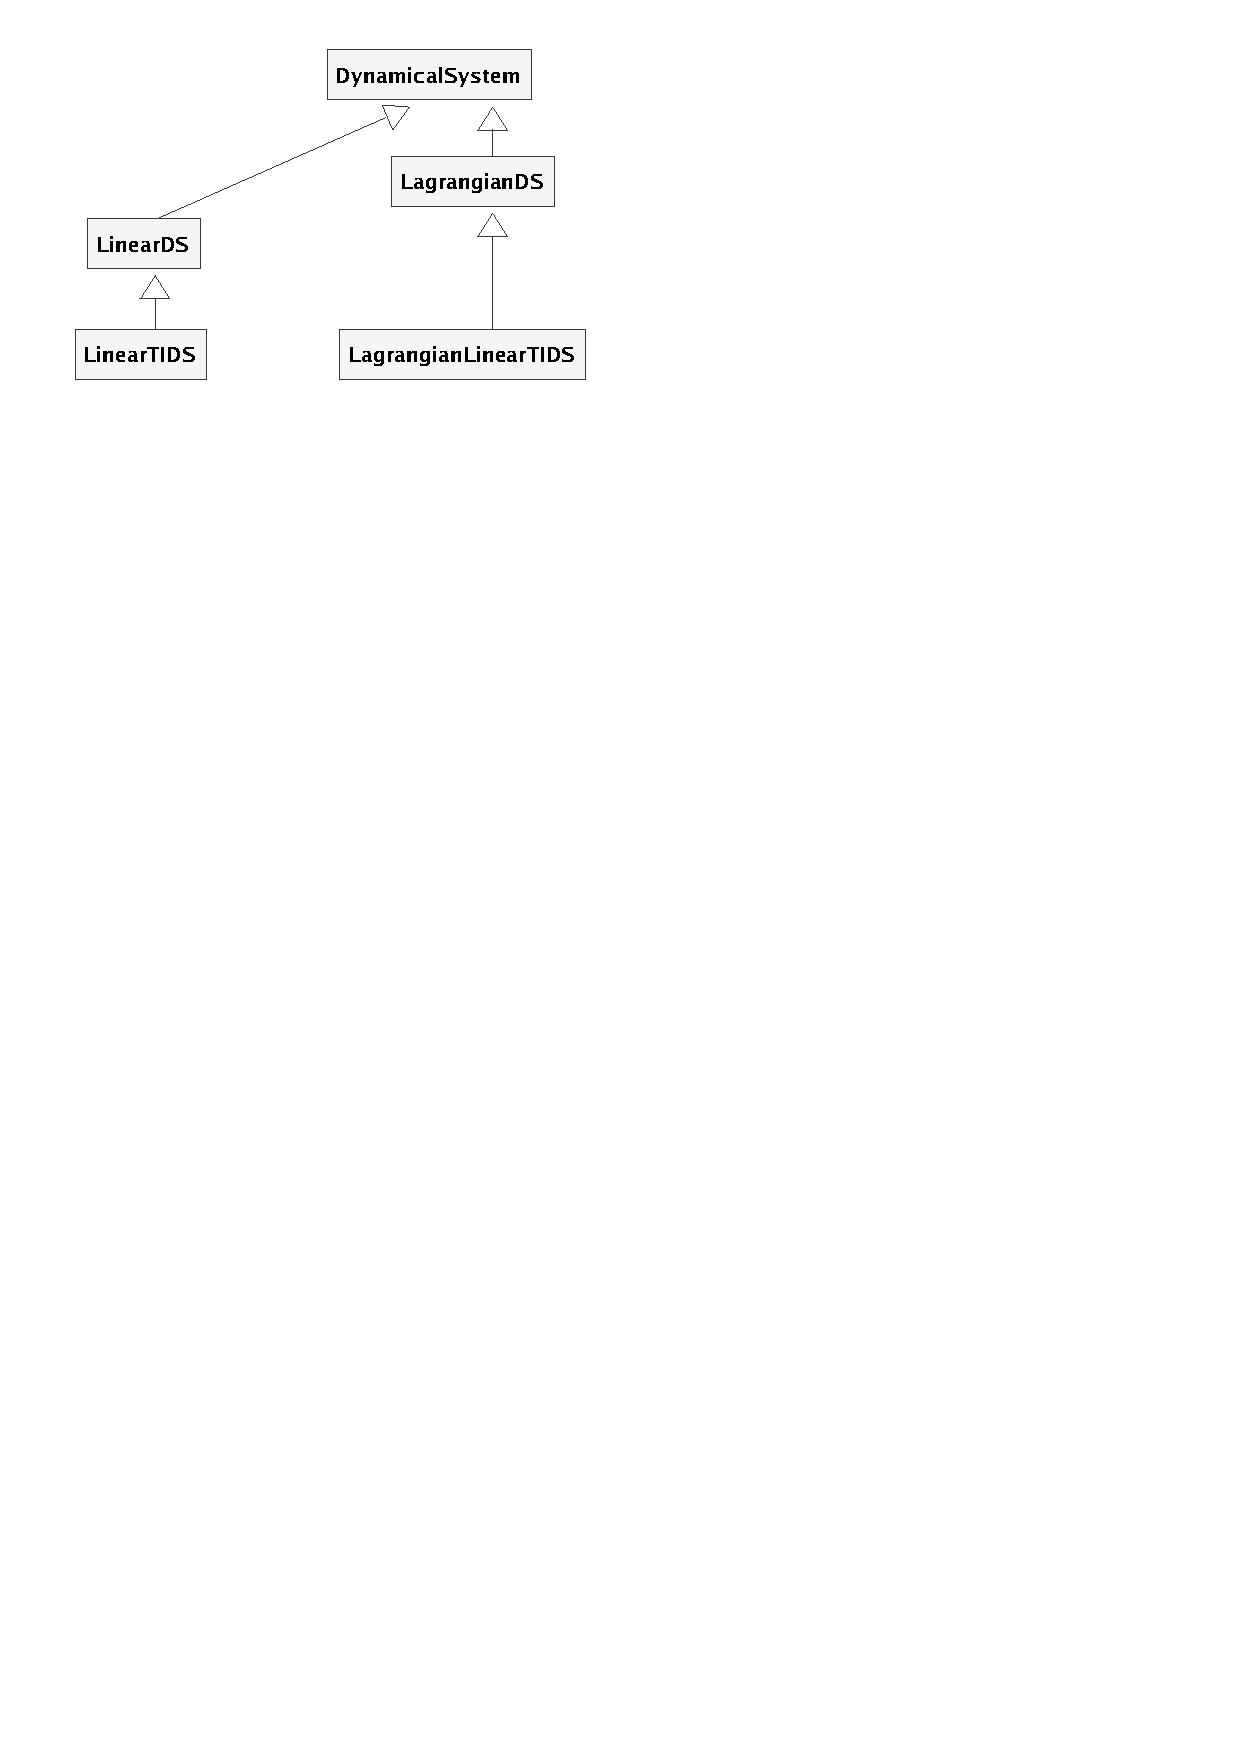
\includegraphics[width=0.3\textwidth]{./DSClassDiagram.pdf}
  \label{DSDiagram}
\end{figure}
% DYNAMICAL SYSTEMS
\section{General non linear first order dynamical systems \\ $\rightarrow$ class \it{DynamicalSystem}}
This is the top class for dynamical systems. All other systems classes derived from this one. \\

A general dynamical systems is described by the following set of $n$ equations, completed with initial conditions:
\begin{eqnarray}
  \dot x &=& f(x,t) + T(x) u(x, \dot x, t) + r \\
  x(t_0)&=&x_0 
\end{eqnarray}

\begin{itemize}
\item $x$: state of the system - Vector of size $n$.
\item $f(x,t)$: vector field - Vector of size $n$.
\item $u(x, \dot x, t)$: control term - Vector of size $uSize$.
\item $T(x)$: $n\times uSize$ matrix, related to control term.
\item $r$: input due to non-smooth behavior - Vector of size $n$.
\end{itemize}

The Jacobian matrix, $\nabla_x f(x,t)$, of $f$ according to $x$, $n\times n$ square matrix, is also a member of the class. \\

Initial conditions are given by the member $x_0$, vector of size $n$. This corresponds to x value when
simulation is starting, ie after a call to strategy->initialize(). \\

There are plug-in functions in this class for $f$ (vectorField), $jacobianX$, $u$ and $T$. All
of them can handle a vector of user-defined parameters. 

% LINEAR DS
\section{First order linear dynamical systems $\rightarrow$ class \it{LinearDS}}

Derived from DynamicalSystem, described by the set of $n$ equations and initial conditions: 
\begin{eqnarray}
  \dot x &=& A(t)x(t)+Tu(t)+b(t)+r \\
  x(t_0)&=&x_0 
\end{eqnarray}
With:
\begin{itemize}
\item $A(t)$: $n\times n$ matrix, state independent but possibly time-dependent.
\item $b(t)$: Vector of size $n$, possibly time-dependent.
\end{itemize}
Other variables are those of DynamicalSystem class. \\
$A$ and $B$ have corresponding plug-in functions. \\

Warning: time dependence for $A$ and $b$ is not available at the time in the simulation part for this kind of dynamical systems. \\

Links with vectorField and its Jacobian are: 
\begin{eqnarray}
  f(x,t) &=& A(t)x(t)+b(t) \\
  jacobianX&=&\nabla_x f(x,t) = A(t) 
\end{eqnarray}

% LAGRANGIANDS
\section{Second order non linear Lagrangian dynamical systems \\  $\rightarrow$ class \it{LagrangianDS}}

Lagrangian second order non linear systems are described by the following set of$nDof$ equations + initial conditions:
\begin{eqnarray}
 M(q) \ddot q + NNL(\dot q, q) + F_{Int}(\dot q , q , t) &=& F_{Ext}(t) + p \\
 q(t_0) &=& q0 \\
 \dot q(t_0) &=& velocity0 
\end{eqnarray}
With:
\begin{itemize}
\item $M(q)$: $nDof\times nDof$ matrix of inertia.
\item $q$: state of the system - Vector of size $nDof$.
\item $\dot q$ or $velocity$: derivative of the state according to time - Vector of size $nDof$.
\item $NNL(\dot q, q)$:  non linear terms, time-independent - Vector of size $nDof$.
\item $F_{Int}(\dot q , q , t)$: time-dependent linear terms - Vector of size $nDof$.
\item $F_{Ext}(t)$: external forces, time-dependent BUT do not depend on state - Vector of size $nDof$.
\item $p$: input due to non-smooth behavior - Vector of size $nDof$.
\end{itemize}

The following Jacobian are also member of this class:
\begin{itemize}
\item jacobianQFInt = $\nabla_q F_{Int}(t,q,\dot q)$ - $nDof\times nDof$ matrix.
\item jacobianVelocityFInt = $\nabla_{\dot q} F_{Int}(t,q,\dot q)$ - $nDof\times nDof$ matrix.
\item jacobianQNNL = $\nabla_q NNL(q,\dot q)$ - $nDof\times nDof$ matrix.
\item jacobianVelocityNNL = $\nabla_{\dot q}NNL(q,\dot q)$ - $nDof\times nDof$ matrix.
\end{itemize}


There are plug-in functions in this class for $F_{int}$, $F_{Ext}$, $M$, $NNL$ and the four Jacobian matrices. All
of them can handle a vector of user-defined parameters. \\

Links with first order dynamical system are: 
\begin{eqnarray}
  n &= &2nDof \\
  x &=&\left[\begin{array}{c}q \\ \dot q \end{array}\right] \\
  f(x,t) &=&  \left[\begin{array}{c} \dot q \\ M^{-1}(F_{Ext}-F_{Int}-NNL) \end{array}\right] \\
  \\
  \nabla_x f(x,t) &=& 
  \left[\begin{array}{cc} 
      0_{nDof\times nDof} & I_{nDof\times nDof} \\
      \nabla_q(M^{-1})(F_{Ext}-F_{Int}-NNL) -M^{-1}\nabla_q(F_{Int}+NNL) &  -M^{-1}\nabla_{\dot q}(F_{Int}+NNL) 
    \end{array}\right] \\
  r &=& \left[\begin{array}{c} 0_{nDof} \\ p \end{array}\right] \\
  u(x,\dot x,t) &=& u_L(\dot q, q, t) \text{  (not yet implemented)} \\
  T(x) &=& \left[\begin{array}{c} 0_{nDof} \\ T_L(q) \end{array}\right] \text{  (not yet implemented)} \\
\end{eqnarray}
With $0_{n}$ a vector of zero of size $n$, $0_{n\times m}$ a $n\times m$ zero matrix and
$I_{n\times n}$, identity $n\times n$ matrix. \\

Warning: control terms ($Tu$) are not fully implemented in Lagrangian systems. This will be part of future version.

% LAGRANGIAN LINEAR TIME INVARIANT DS
\section{Second order linear and time-invariant Lagrangian dynamical systems $\rightarrow$ class \it{LagrangianLinearTIDS}}
\label{Sec:LagrangianLineatTIDS}
\begin{eqnarray}
M \ddot q + C \dot q + K q =  F_{Ext}(t) + p
\end{eqnarray}

With:
\begin{itemize}
\item $C$: constant viscosity $nDof\times nDof$ matrix 
\item $K$: constant rigidity $nDof\times nDof$ matrix 
\end{itemize}

And: 
\begin{eqnarray}
F_{Int} &=& C \dot q + K q \\
NNL &=& 0_{nDof} 
\end{eqnarray}



\chapter{Dynamical Systems implementation in Siconos.}

\begin{table}[!ht]
  \begin{tabular}{|l|l|}
    \hline
    author  & F.  P\'erignon \\
    \hline
    date    & November 7, 2006 \\ 
    \hline
    version & Kernel 1.3.0 \\
    \hline
  \end{tabular}
\end{table}




\section{Introduction}
This document is only a sequel of notes and remarks on the way Dynamical Systems are implemented in Siconos.\\
It has to be completed, reviewed, reorganized etc etc for a future Developpers'Guide. \\
See also documentation in Doc/User/DynamicalSystemsInSiconos for a description of various dynamical systems types.

\section{Class Diagram}
There are four possible formulation for dynamical systems in Siconos,
two for first order systems and two for second order Lagrangian systems. The main class is DynamicalSystem, all other derived from this one, as shown in the following diagram:
\begin{figure}[htbp]
  \centering
 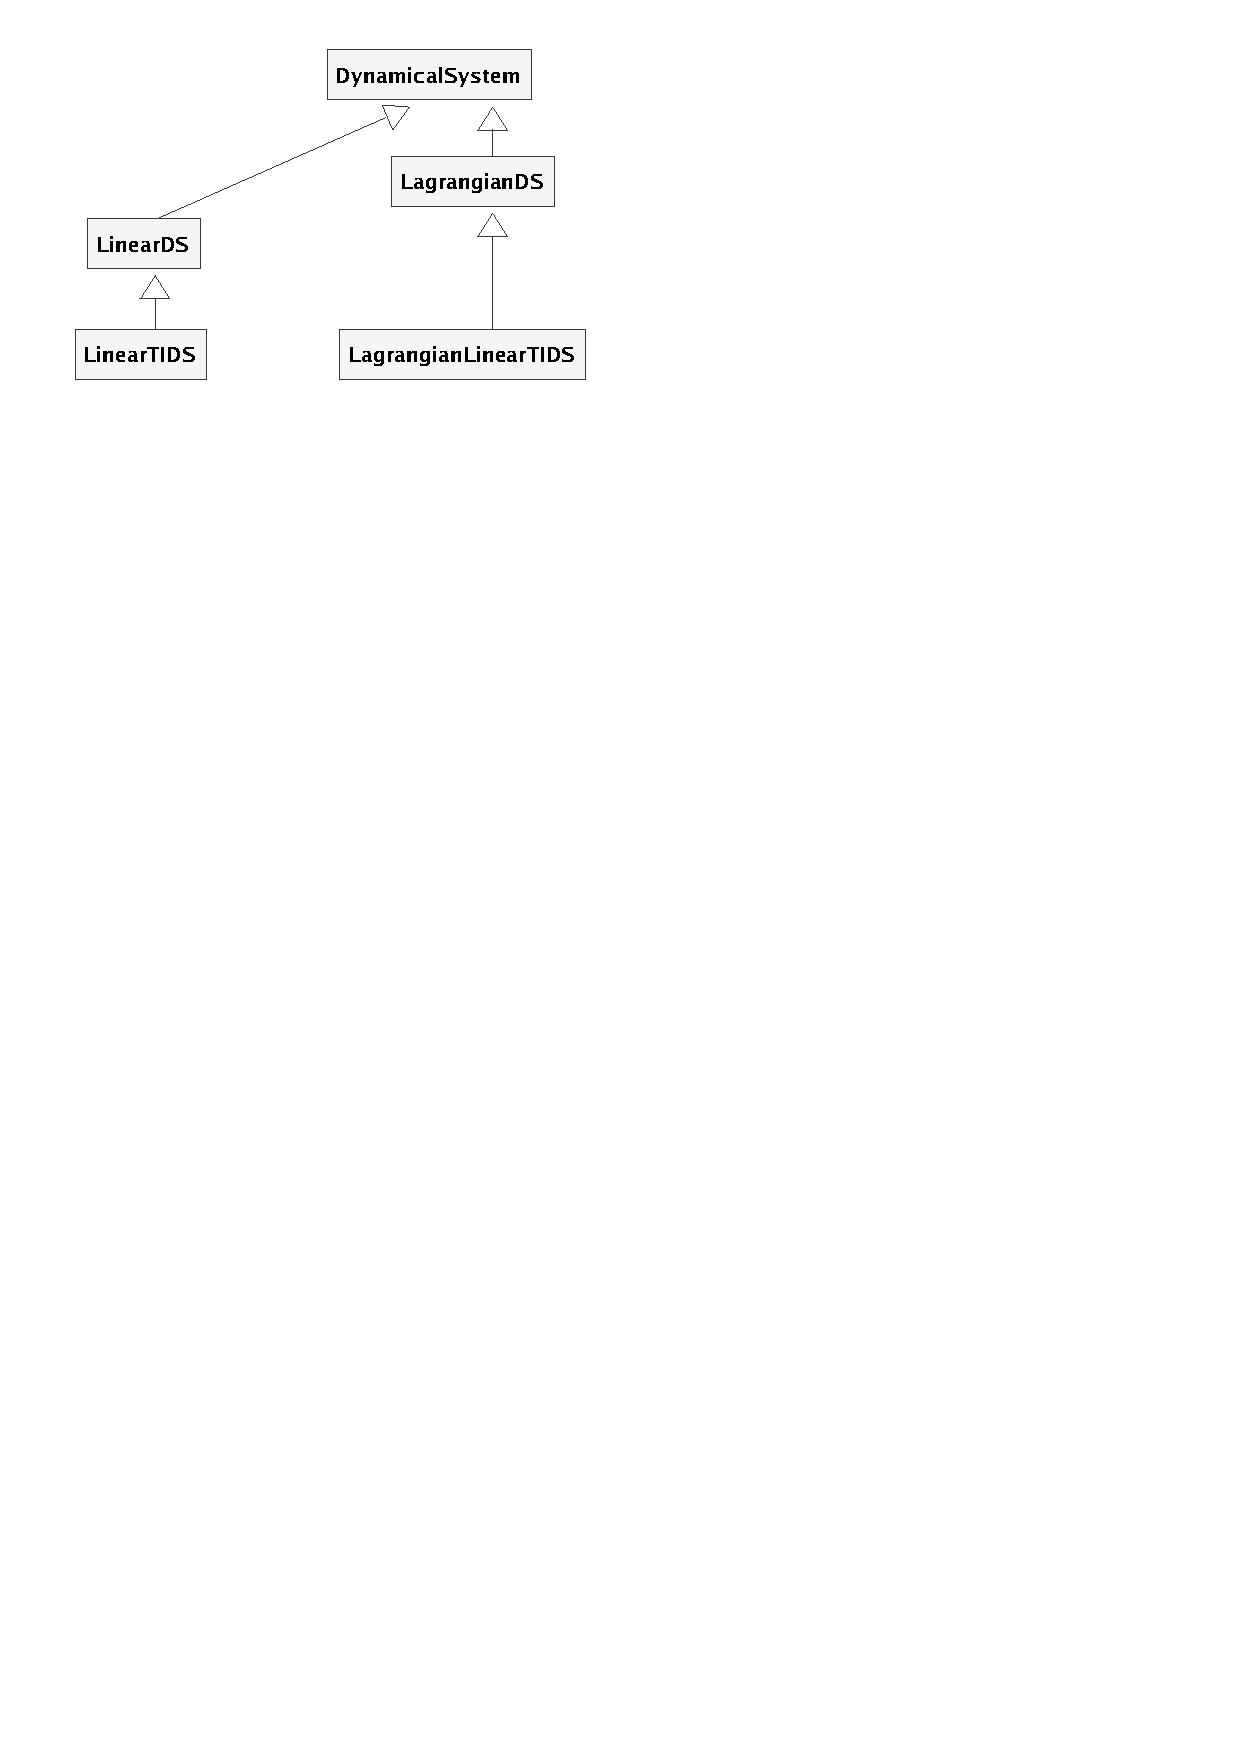
\includegraphics[width=0.3\textwidth]{./DSClassDiagram.pdf}
  \label{DSDiagram}
\end{figure}
% DYNAMICAL SYSTEMS

\section{Construction}

Each constructor must:
\begin{itemize}
\item initialize all the members of the class and of the top-class if it exists
\item allocate memory and set value for all required inputs
\item allocate memory and set value for optional input if they are given as argument (in xml for example)
\item check that given data are coherent and that the system is complete (for example, in the LagrangianDS
if the internal forces are given as a plug-in, their Jacobian are also required. If they are not given, this leads to an exception).
\end{itemize}

No memory allocation is made for unused members $\Rightarrow$ requires if statements in simulation.  (if!=NULL ...).\\

\subsection{DynamicalSystem}

{\bf Required data:}\\
n, x0, f, jacobianXF \\
{\bf Optional:}\\
T,u \\

\textbf{Always allocated in constructor:} \\
x, x0, xFree, r, rhs, jacobianXF

Warning: default constructor is always private or protected and apart from the others and previous rules or remarks do not always apply to it. 
This for DS class and any of the derived ones. 

\subsection{LagrangianDS}

\textbf{Required data:}\\
ndof, q0, velocity0, mass \\
\textbf{Optional:}\\
fInt and its Jacobian, fExt, NNL and its Jacobian. \\

\textbf{Always allocated in constructor:} \\
mass, q, q0, qFree, velocity, velocity0, velocityFree, p. \\
All other pointers to vectors/matrices are set to NULL by default. \\
Memory vectors are required but allocated during call to initMemory function. 

Various rules:
\begin{itemize}
\item fInt (NNL) given as a plug-in $\Rightarrow$ check that JacobianQ/Velocity are present (matrices or plug-in)
\item any of the four Jacobian present $\Rightarrow$ allocate memory for block-matrix jacobianX  (connectToDS function)
\item 
\end{itemize}

check: end of constructor or in initialize? \\
computeF and JacobianF + corresponding set functions: virtual or not? \\


\section{Specific flags or members}

\begin{itemize}
\item isAllocatedIn: to check inside-class memory allocation
\item isPlugin: to check if operators are computed with plug-in or just directly set as a matrix or vector
\item workMatrix: used to save some specific matrices in order to avoid recomputation if possible (inverse of mass ...)
\end{itemize}

\section{plug-in management}
DynamicalSystem class has a member named parameterList which is a $map<string, SimpleVector*>$, ie a list of
pointers to SimpleVector*, with a string as a key to identified them. 
For example, $parametersList["mass"]$ is a SimpleVector*, which corresponds to the last argument given in 
mass plug-in function. \\
By default, each parameters vectors must be initialized with a SimpleVector of size 1, as soon as the plug-in is
declared. Moreover, to each vector corresponds a flag in isAllocatedIn map, to check if the corresponding vector has been 
allocated inside the class or not. \\ 
For example, in DynamicalSystem, if $isPlugin["vectorField"]==true$, then, during call to constructor or set function,
it is necessary to defined the corresponding parameter: \\
$parametersList["vectorField"] = new SimpleVector(1)$ \\
and to complete the $isAllocatedIn$ flag: \\
$isAllocatedIn["parameter_for_vectorField"] = true$. \\

\chapter{Interactions}
\begin{table}[!ht]
  \begin{tabular}{|l|l|}
    \hline
    author  & F.  P\'erignon \\
    \hline
    date    & November 7, 2006 \\ 
    \hline
    version & Kernel 1.3.0 \\
    \hline
  \end{tabular}
\end{table}

\section{Introduction}
This document is only a sequel of notes and remarks on the way Interactions are implemented in Siconos.\\
It has to be completed, reviewed, reorganized etc etc for a future Developpers'Guide. \\
See also documentation in Doc/User/Interaction.

\section{Class Diagram}

\section{Description}

\begin{ndrfp} 
review of interactions (for EventDriven implementation) 17th May 2006.
\end{ndrfp}

\bei
\item variable \varcpp{nInter} renamed in \varcpp{interactionSize}: represents the size of \varcpp{y} and \varcpp{$\lambda$}. NOT the number of relations !! \\
\item add a variable \varcpp{nsLawSize} that depends on the non-smooth law type.\\
Examples:
\bei
\item NewtonImpact -> \varcpp{nsLawSize} = 1
\item Friction 2D  -> \varcpp{nsLawSize} = 2
\item Friction 3D  -> \varcpp{nsLawSize} = 3
\item ... 
\item \varcpp{nsLawSize} = n with n dim of matrix D in :
$y=Cx+D\lambda$, D supposed to be a full-ranked matrix. \\
Warning: this case is represented by only one relation of size n. 
\ei
\item \varcpp{numberOfRelations}: number of relations in the interaction, \varcpp{numberOfRelations} = $\Frac{\varcpp{interactionSize}}{\varcpp{nsLawSize}}$.
\ei


\chapter{Notes on the Non Smooth Dynamical System construction}
\begin{table}[!ht]
  \begin{tabular}{|l|l|}
    \hline
    author  & F.  P\'erignon \\
    \hline
    date    & November 7, 2006 \\ 
    \hline
    version & Kernel 1.3.0 \\
    \hline
  \end{tabular}
\end{table}

\section{Introduction}

\section{Class Diagram}

\section{Description}

Objects must be constructed in the following order: 
\bei
\item DynamicalSystems
\item NonSmoothLaw: depends on nothing
\item Relation: no link with an interaction during construction, this will be done during initialization. 
\item Interaction: default constructor is private and copy is forbidden. Two constructors: xml and from data. Required data are a DSSet, a NonSmoothLaw and
a Relation (+ dim of the Interaction and a number). \\
Interaction has an initialize function which allocates memory for y and lambda, links correctly the relation and initializes it .... This function is called at the 
end of the constructor. That may be better to call it in simulation->initialize? Pb: xml constructor needs memory allocation for y and lambda if they are
provided in the input xml file. 
\item NonSmoothDynamicalSystem: default is private, copy fobidden. Two constructors: xml and from data. Required data are the DSSet and the InteractionsSet.
The topology is declared and constructed (but empty) during constructor call of the nsds, but initialize in the Simulation, this because it can not be initialize until the nsds has been fully described (ie this to allow user to add DS, Inter ...) at any time in the model, but before simulation initialization). 

\ei

\section{misc}

\bei 
\item no need to keep a number for Interactions? Only used in xml for OSI, to know which Interactions it holds.
\item pb: the number of saved derivatives for y and lambda in Interactions is set to 2. This must depends on the relative degree which is computes during
Simulation initialize and thus too late. It is so not available when memory is allocated (Interaction construction). Problem-> to be reviewed.
\ei 


\chapter{OneStepIntegrator and derived classes.}
\begin{table}[!ht]
  \begin{tabular}{|l|l|}
    \hline
    author  & F.  P\'erignon \\
    \hline
    date    & November 7, 2006 \\ 
    \hline
    version & Kernel 1.3.0 \\
    \hline
  \end{tabular}
\end{table}

\section{Introduction}
This document is only a sequel of notes and remarks on the way OneStepIntegrators are implemented in Siconos.\\
It has to be completed, reviewed, reorganized etc etc for a future Developpers'Guide. \\
See also documentation in Doc/User/OneStepIntegrator for a description of various OSI.

\section{Class Diagram}

\section{Misc}

OSI review for consistency between Lsodar and Moreau:
\begin{itemize}
\item add set of DynamicalSystem*
\item add set of Interaction* 
\item add link to strategy that owns the OSI
\item remove td object in OSI -> future: replace it by a set of td (one per ds)
\item add strat in constructors arg list
\end{itemize}



osi -> strat -> Model -> nsds -> topology \\
osi -> strat -> timeDiscretisation \\

let a timeDiscretisation object in the OSI? set of td (one per ds)? \\
create a class of object that corresponds to DS on the simulation side ? \\
will contain the DS, its discretization, theta for Moreau ... ? \\ 
Allow setStrategyPtr operation? Warning: need reinitialisation. \\


Required input by user: \\
\begin{itemize}
\item list of DS or list of Interactions ? 
\item pointer to strategy
\item ...
\end{itemize}

\section{Construction}

Each constructor must:

\begin{itemize}
\item
\end{itemize}

\subsection{Moreau}

Two maps: one for W, and one for theta. To each DS corresponds a theta and a W. \\
Strategy arg in each constructor.

\textbf{Required data:}\\

\textbf{Optional:}\\

\textbf{Always allocated in constructor:} \\

Warning: default constructor is always private or protected and apart from the others and previous rules or remarks do not always apply to it. 

\subsection{Lsodar}

\textbf{Required data:}\\

\textbf{Optional:}\\

\textbf{Always allocated in constructor:} \\

\chapter{First Order Nonlinear Relation }

\begin{table}[!ht]
  \begin{tabular}{|l|l|}
    \hline
    author  & 0. Bonnefon \\
    \hline
    date    & July, 1 2009 \\ 
    \hline
    version & Kernel 3.0.0 \\
    \hline
  \end{tabular}
\end{table}

\chapter{Computation of the number of Index Set and various levels}
\begin{table}[!ht]
  \begin{tabular}{|l|l|}
    \hline
    author  & V. Acary \\
    \hline
    date    & Septembre 16, 2011 \\ 
    \hline
    version & Kernel 3.3.0 \\
    \hline
  \end{tabular}
\end{table}


In this chapter, we give some hints on the automatic computation of the number of index sets, the number of derivatives in the {\tt Interaction} and the levelMin and LevelMax.


\section{Why is the  relative degree not relevant ?}
In this section, we give a very brief overview of the notion of relative degree.

\subsection{First order Linear complementary systems}

 A  Linear Complementarity System (LCS) is defined by
\begin{equation}
  \label{eq:LCS-bis}
  \begin{cases}
    \dot x = A x +B \lambda \\
     y = C x + D \lambda\\
    0 \leq  y \perp \lambda \geq 0 \\
  \end{cases}
\end{equation} 
 \begin{definition}[Relative degree in the SISO case]
      Let us consider a linear system in state representation given by the quadruplet $(A,B,C,D) \in \RR^{n\times n}\times\RR^{n \times m}\times \RR^{m\times n}\times\RR^{m\times m} $:
      \begin{equation}
        \label{eq:LS}
        \begin{cases}
          \dot x = A x +B \lambda \\
          y = C x + D \lambda
        \end{cases}
      \end{equation}
      \begin{itemize}
      \item In the Single Input/ Single Output (SISO) case ($m=1$), the relative
        degree is defined by the first non zero Markov parameters :
        \begin{equation}
          \label{eq:Markov-Parameter}
          D, CB, CAB, CA^2B, \ldots, CA^{r-1}B, \ldots
        \end{equation}
      \item In the multiple input/multiple output (MIMO) case ($m>1$), an \textit{uniform} relative degree is defined as follows.
        If $D$ is non singular, the relative degree is equal to $0$. Otherwise, it is assumed to be the first positive integer $r$ such that 
        \begin{equation}
          \label{eq:mimo-r}
          CA^{i}B =0, \quad i=0\ldots q-2
        \end{equation}
        while
        \begin{equation}
          \label{eq:mimo-r2}
          CA^{r-1}B \text{ is non singular}.
        \end{equation}
      \end{itemize}
    \end{definition}
    The Markov parameters arise naturally when we derive with respect
    to time the output $y$,
    \begin{eqnarray*}
      \label{eq:y-derive}
      y &=& C x + D \lambda \\
      \dot y &=& CA x + CB \lambda, \text{ if } D= 0  \\
      \ddot y &=& CA^2 x + CAB \lambda, \text{ if }  D=0, CB=0\\
      &\ldots& \\
      y^{(r)} &=& CA^{r} x + CA^{r-1}B \lambda, \text{ if } D=0, CB=0, CA^{r-2}B=0, r=1\ldots r-2 \\
      &\ldots&
    \end{eqnarray*}
    and the first non zero Markov parameter allows us to define the
    output $y$ directly in terms of the input $\lambda$.

In continuous time, the nature of solutions depends strongly on the relative degree. When we want to perform the time--integration of such systems, we need also to reduce the relative degree or to known it to correctly operate.

We can observe that the relative degree $0$ is well defined only by the relation ($D$ nonsingular) and by the nonsmooth law. Indeed, let us imagine that the nonsmooth law is defined by $0\leq\dot y \perp \lambda \geq 0 $. We can easily see that the relative degree is reduced.

In the MIMO, the computation of non uniform relative degree is hard task. This is also the case for nonlinear systems.



\subsection{Second order Lagrangian systems}


Let us consider a second order linear and time-invariant Lagrangian dynamical system (see \S~\ref{Sec:LagrangianLineatTIDS})
\begin{equation}
  \label{eq:rd1}
  \begin{cases}
    M \dot v + C v + K q = F_{Ext}(t) + p \\
    \dot q = v
  \end{cases}
\end{equation}
together with a Lagrangian linear relation
\begin{equation}
  y= Cq + e + D \lambda + Fz,
  \label{eq:rd2}
\end{equation}
\begin{equation}
  p = C^t \lambda
\label{eq:rd3}  
\end{equation}
and a simple nonsmooth law,
\begin{equation}
  0\leq y \perp \lambda \geq 0
\label{eq:rd4}  
\end{equation}

If $D>0$, the relative degree is uniformly zero and the system can be solved without deriving the output~(\ref{eq:rd2}). Indeed, we known that the solution of the LCP
\begin{equation}
  0\leq Cq + e + D \lambda + Fz, \perp \lambda \geq 0
\label{eq:rd5}  
\end{equation}
is unique and Lipschitz with respect to $q$. It can be denoted as $\lambda(q) = \mbox{SOL}(D,Cq + e +Fz)$. Therefore, the differential equation~(\ref{eq:rd1}) reduces to a standard ODE with a Lipschitz RHS
 \begin{equation}
  \label{eq:rd6}
  \begin{cases}
    M \dot v + C v + K q = F_{Ext}(t) + C^t \lambda(q)  \\
    \dot q = v
  \end{cases}
\end{equation}

In the case that we deal with unilateral contact, we usually have $D=0$ and the relative degree of the system is $2$. In this case, the output has to be differentiated as
\begin{equation}
  \label{eq:rd7}
   \dot y= C \dot q,
\end{equation}
and an impact law has to added, for instance the newton's impact law
\begin{equation}
  \label{eq:rd8}
  \text{ if } y=0, \text{ when } \dot y^+= -e y^-
\end{equation}
In the same vein, the equations of motion (\ref{eq:rd1}) is not sufficient since the velocity may encounter jumps. The dynamics is usually replaced by a measure differential equation of the form
\begin{equation}
  \label{eq:rd10}
  \begin{cases}
    M dv + C v^+(t) dt + K q(t) dt = F_{Ext}(t)dt + di \\
    \dot q = v
  \end{cases}
\end{equation}
where $di$ is the measure that can be related to $p$ thanks to
\begin{equation}
  \label{eq:rd11}
  di = p dt + \sigma \delta _{t^*}
\end{equation}
is only one jump is expected at ${t^*}$.


\subsection{Conclusion for the implementation}
From the continuous time mathematical analysis, the relative degree is very important to know if we have to compute the derivatives of the output $y^{(n)}$ and to consider various levels for the input $p , \sigma, ....$

However in the numerical practice,  the time --discretization makes an assumption on the relative degree and treats the nonsmooth law at different levels. The resulting time discretized system posseses more or less variables.

Consider for instance  (\ref{eq:rd1}) in the case of the Moreau scheme
\begin{subnumcases}{\label{eq:MoreauTS}}
  M(v_{k+1}-v_k)  + h  (K q_{k+\theta}+ C v_{k+\theta}) = p_{k+1} = G(q_{k+1}) \lambda_{k+1},\quad\,\\[1mm] 
  q_{k+1} = q_{k} + h v_{k+\theta}, \quad \\[1mm]
  \dot y_{k+1} = G^\top(q_{k+1})\, v_{k+1} \\[1mm]
  \begin{array}{l}
    \text{if }\quad\bar y^\alpha_{k+1} \leq 0 \text{ then } 0 \leq \dot y^\alpha_{k+1} + e  \dot y^\alpha_{k} \perp \lambda^\alpha_{k+1}  \geq 0, \\[1mm]
    \text{otherwise  } \lambda^\alpha_{k+1}  =0.\label{eq:MoreauTSd}
  \end{array}, \alpha \in \mathcal I
\end{subnumcases} 
and the Schatzman--Paoli  scheme
\begin{subnumcases}{}
  M(q_{k+1}-2q_{k}+q_{k-1})  + h^2 (K q_{k+\theta}+ C v_{k+\theta})  =  p_{k+1},\quad\,\\ \notag\\ 
  v_{k+1}=\Frac{q_{k+1}-q_{k-1}}{2h}, \\ \notag \\
  y_{k+1} = h\left(\Frac{q_{k+1}+e q_{k-1}}{1+e}\right) \\
  p_{k+1}= G\left(\Frac{q_{k+1}+e q_{k-1}}{1+e}\right) \lambda_{k+1} \\
  0 \leq y_{k+1}  \perp\lambda_{k+1} \geq 0 .
\end{subnumcases}

We can see easily that the number of derivatives (or levels) that we store for $y$ and $\lambda$ is independent on the relative degree but is chosen by the {\tt OneStepIntegrator} with respect to the type of systems.

\section{How to define and compute the various levels and the number of indexSets }

\subsection{$y$ related variables}

The size of the vector {\tt y} in the {\tt Interaction} depends on
\begin{itemize}
\item the {\tt  OneStepIntegrator} type.
  \begin{itemize}
  \item see the difference between the Moreau and Schatzman Paoli
    scheme,
  \item plan the time--discontinuous Galerkin scheme
  \item plan the Higher Order Moreau sweeping process (HOSP)
  \end{itemize}
\item the {\tt  Simulation} type.
  \begin{itemize}
  \item In {\tt Timestepping} or {\tt Event-driven} we do not need the same number of stored $y$
  \end{itemize}

\item the {\tt NonSmoothLaw} type.
  \begin{itemize}
  \item If we consider some cases with or without friction in {\tt
      Timestepping} or {\tt Event-driven}, we need to adapt the number
    of stored $y$
  \end{itemize}

\end{itemize}

Since the various levels of  {\tt y} are used to build the index sets we will need from $0$ to a computed size that depends on the previous criteria. Only a part will be used in the {\tt OneStepNSProblem}.

\subsection{$\lambda$ related variables}

The size of the vector {\tt lambda} in the {\tt Interaction} depends on the same criteria than in the previous section.  Only, the number of lambda is not the same as {\tt y} since a multiplier {\tt lambda[i]} is not necessarily related to {\tt y[i]}

\section{Rules for implementation}

We can define new members in {\tt Interaction}:
\begin{itemize}
\item {\tt \_lowerlevelForOutput}, this value is to $0$ by default
\item {\tt \_upperlevelForOutput},  this value must be computed at initialization with respect to the previous criteria
\item {\tt \_lowerlevelForInput},  this value must be computed at initialization with respect to the previous criteria
\item {\tt \_upperlevelForInput},  this value must be computed at initialization with respect to the previous criteria
\end{itemize}




This level are computed in {\tt Simulation::ComputeLevelsForInputAndOutput}. A visitor is used for the {\tt OneStepIntegrator}. Furthermore, four global levels are computed 
\begin{itemize}
\item {\_levelMinForOutput} this value is the minimum level for the output {\tt Interaction::\_lowerlevelForOutput}  for all the interactions
\item {\_levelMaxForOutput} this value is the maximum level for the output {\tt Interaction::\_upperlevelForOutput}  for all the interactions
\item {\_levelMinForInput} this value is the minimum level for the output {\tt Interaction::\_lowerlevelForInput}  for all the interactions
\item {\_levelMaxForInput} this value is the maximum level for the output {\tt Interaction::\_upperlevelForInput}  for all the interactions
\end{itemize}




\begin{itemize}
\item the values {\tt y[i]} must be initialized from {\tt \_lowerlevelForOutput} to {\tt \_upperlevelForOutput}.
\item the values {\tt lamdba[i]} must be initialized from {\tt \_lowerlevelForInput} to  {\tt \_upperlevelForInput}.
\item the values {\tt y[i]} in {\tt Interaction} must be used in priority to store the i-th derivative of $y$. When it is needed, higher index $i$ can be used for other triggering variables. For instance, for an Event--Driven scheme with a Lagrangian systems with friction, sliding velocity must be stored.
\item the values of {\tt lamdba[i]} must stored the various multiplier for the nonsmooth law. We affect the same index $i$ as for the level of {\tt y[i]} present in the corresponding nonsmooth law.
\item The number of {\tt IndexSets} should follows {\tt \_levelMaxForY}.
\end{itemize}



For the dynamical systems :
\begin{itemize}
\item The number of levels for {\tt \_r} and {\tt \_p} in the DS should follow {\tt \_lowerlevelForInput} and {\tt \_upperlevelForOutput} of the associated interactions. This is done in {\tt Interaction::initialize}.
\item A new variable should be added in the LagrangianDS to store the multiplier at the position level ({\tt \_tau} ?) to avoid the use of {\tt \_p[0]}. Indeed, we will continue to assume that {\tt \_p} is the input in the equation of motion. For {\tt lambda} we can  use {\tt lambda[0]} 
\end{itemize}

TODO LIST AND QUESTIONS
\begin{itemize}
\item What about the case of multiples interactions on a DS with various {\tt \_lowerlevelForInput} and {\tt \_upperlevelForOutput} ? Normally, all the levels should be correctly initialized thanks to the proposed implementation (r2821)
\item {\tt DynamicalSystem::\_r} should be a VectorOfVectors
\item {\tt DynamicalSystem::\_r} is split in {\tt LagrangianDS}. a first part is {\tt LagrangianDS::\_p}. The other is not implemented !! {\tt LagrangianDS::\_tau} ?
\end{itemize}


%%% Local Variables: 
%%% mode: latex
%%% TeX-master: "DevNotes"
%%% End: 



\chapter{Newton's linearization for First Order Systems}
 \begin{table}[!ht]
  \begin{tabular}{|l|l|}
    \hline
    author  & O.Bonnefon, V. Acary\\
    \hline
    date    & Sept, 07, 2007 \\ 
    last update        & Feb, 2011 \\
                       & April, 2014 \\
    \hline
    version &  \\
    \hline
  \end{tabular}
\end{table}



This section is devoted to the implementation and the study  of the algorithm. The interval of integration is $[0,T]$, $T>0$, and a grid $t_{0}=0$, $t_{k+1}=t_{k}+h$, $k \geq 0$, $t_{N}=T$ is constructed. The approximation of a function $f(\cdot)$ on $[0,T]$ is denoted as $f^{N}(\cdot)$, and is a piecewise constant function, constant on the intervals $[t_{k},t_{k+1})$. We denote $f^{N}(t_{k})$ as $f_{k}$. The time-step is $h>0$. 


\section{Various first order dynamical systems with input/output relations}

\paragraph{FirstOrderR. Fully nonlinear case}
Let us introduce the following system, 
\begin{equation}
\begin{array}{l}
M \dot{x}(t) = f(x(t),t) + r(t)  \\[2mm]
y(t) = h(t,x(t),\lambda (t)) \\[2mm]
r(t) = g(t,x(t),\lambda (t) ) \\[2mm]
\end{array}
\label{first-DS}
\end{equation}
where $\lambda(t) \in \RR^m$  and $y(t) \in \RR^m$ are  complementary variables related through a multi-valued mapping.   According to the class of systems, we are studying, the function $f$ and $g$ are defined by a fully nonlinear framework or by affine functions. We have decided to present the time-discretization in its full generality and specialize the algorithms for each cases in Section~\ref{Sec:Spec}. This fully nonlinear case is not  implemented in Siconos yet. This fully general case is not yet implemented in Siconos.

This case is implemented in Siconos with the relation {\tt FirstOrderR} using the subtype {NonLinearR}

\paragraph{FirstOrderType1R}
Let us introduce a new notation,
\begin{equation}
\begin{array}{l}
M \dot{x}(t) = f(x(t),t) + r(t)  \\[2mm]
y(t) = h(t,x(t)) \\[2mm]
r(t) = g(t,\lambda (t) ) \\[2mm]
\end{array}
\label{first-DS1}
\end{equation}
This case is implemented in Siconos with the relation {\tt FirstOrderType1R}.



\paragraph{FirstOrderType2R}
Let us introduce a new notation, 
\begin{equation}
\begin{array}{l}
M \dot{x}(t) = f(x(t),t) + r(t)  \\[2mm]
y(t) = h(t,x(t),\lambda (t)) \\[2mm]
r(t) = g(t,\lambda (t) ) \\[2mm]
\end{array}
\label{first-DS2}
\end{equation}
This case is implemented in Siconos with the relation {\tt FirstOrderType2R}.




\paragraph{Linear case }Let us introduce a new notation, 
\begin{equation}
\begin{array}{l}
M \dot{x}(t) = Ax(t) + r(t)  +b(t)\\[2mm]
y(t) = h(x(t),\lambda (t),z) = Cx + Fz + D \lambda  \\[2mm]
r(t) = g(t,\lambda (t) ) = B \lambda \\[2mm]
\end{array}
\label{first-DS3}
\end{equation}


\section{Time--discretizations}



\subsection{Standard $\theta-\gamma$ scheme.}
Let us now proceed with the time discretization of (\ref{first-DS3}) by a fully implicit scheme : 
\begin{equation}
  \begin{array}{l}
    \label{eq:toto1}
     M x_{k+1} = M x_{k} +h\theta f(x_{k+1},t_{k+1})+h(1-\theta) f(x_k,t_k) + h \gamma r(t_{k+1})
     + h(1-\gamma)r(t_k)  \\[2mm]
     y_{k+1} =  h(t_{k+1},x_{k+1},\lambda_{k+1}) \\[2mm]
     r_{k+1} =  g(t_{k+1},x_{k+1},\lambda_{k+1})\\[2mm]
     \mbox{NsLaw} ( y_{k+1} , \lambda_{k+1})
  \end{array}
\end{equation}
where $\theta = [0,1]$ and $\gamma \in [0,1]$. As in \cite{acary2008}, we call the problem \eqref{eq:toto1} the ``one--step nonsmooth problem''.

In the Siconos/Kernel module, the use of $\gamma$  is activated in the class {\tt EulerMoreauOSI} by the boolean {\tt \_useGamma}.



 This time-discretization is slightly more general than a standard implicit Euler scheme. The main discrepancy lies in the choice of a $\theta$-method to integrate the nonlinear term. For $\theta=0$, we retrieve the explicit integration of the smooth and  single valued term $f$. Moreover for $\gamma =0$, the term $g$ is explicitly evaluated. The flexibility in the choice of $\theta$ and $\gamma$ allows the user to improve and control the accuracy, the stability and the numerical damping of the proposed method. For instance, if the smooth dynamics given by $f$ is stiff, or if we have to use big step sizes for practical reasons, the choice of $\theta > 1/2$ offers better stability with the respect to $h$.

\subsection{Full $\theta-\gamma$ scheme}

Another possible time--discretization is as follows.
\begin{equation}
  \begin{array}{l}
    \label{eq:toto1-ter}
    M x_{k+1} = M x_{k} + h\theta f(x_{k+1},t_{k+1})+h(1-\theta) f(x_k,t_k) + h r(t_{k+\gamma}) \\[2mm]
    y_{k+\gamma} = h(t_{k+\gamma},x_{k+\gamma},\lambda _{k+\gamma}) \\[2mm]
    r_{k+\gamma} = g(t_{k+\gamma},x_{k+\gamma},\lambda _{k+\gamma})\\[2mm]
    \mbox{NsLaw} ( y_{k+\gamma} , \lambda_{k+\gamma})
  \end{array}
\end{equation}
We call the scheme~(\ref{eq:toto1-ter}) the full $\theta-\gamma$ scheme since it uses also the evaluation at $t_{k+\gamma}$ for the relation.

In the Siconos/Kernel module, the time--stepping scheme is activated in the class {\tt EulerMoreauOSI} by the boolean {\tt \_useGammaForRelation}.


Another possibility for the time discretization in the nonlinear case would be
\begin{equation}
  \begin{array}{l}
    \label{eq:toto1-quat}
    M x_{k+1} = M x_{k} +h f(x_{k+\theta},t_{k+\theta}) + h r(t_{k+\gamma}) \\[2mm]
    y_{k+\gamma} =  h(t_{k+\gamma},x_{k+\gamma},\lambda _{k+\gamma}) \\[2mm]
    r_{k+\gamma} = g(t_{k+\gamma},x_{k+\gamma},\lambda _{k+\gamma})\\[2mm]
    \mbox{NsLaw} ( y_{k+\gamma} , \lambda_{k+\gamma})
  \end{array}
\end{equation}
This scheme has not been yet implemented in Siconos/Kernel.

\clearpage
\section{Newton's linearization of~(\ref{eq:toto1})} 


Due to the fact that  two of the  studied classes of systems that are studied in this paper are affine functions in terms of $f$ and $g$, we propose to solve the "one--step nonsmooth problem'' (\ref{eq:toto1}) by performing an external Newton linearization.

 \paragraph{Newton's linearization of the first line of~(\ref{eq:toto1})} The first line of the  problem~(\ref{eq:toto1}) can be written under the form of a residue $\mathcal R$ depending only on $x_{k+1}$ and $r_{k+1}$ such that 
\begin{equation}
  \label{eq:NL3}
  \mathcal R (x_{k+1},r _{k+1}) =0
\end{equation}
with 
\begin{equation}
\mathcal R(x,r) = M(x - x_{k}) -h\theta f( x , t_{k+1}) - h(1-\theta)f(x_k,t_k) - h\gamma r
- h(1-\gamma)r_k.
\end{equation}
The solution of this system of nonlinear equations is sought as a limit of the sequence $\{ x^{\alpha}_{k+1},r^{\alpha}_{k+1} \}_{\alpha \in \NN}$ such that
 \begin{equation}
   \label{eq:NL7}
   \begin{cases}
     x^{0}_{k+1} = x_k \\ \\
     r^{0}_{k+1} = r_k \\ \\
     \mathcal R_L( x^{\alpha+1}_{k+1},r^{\alpha+1}_{k+1}) = \mathcal
     R(x^{\alpha}_{k+1},r^{\alpha}_{k+1})  + \left[ \nabla_{x} \mathcal
     R(x^{\alpha}_{k+1},r^{\alpha}_{k+1})\right] (x^{\alpha+1}_{k+1}-x^{\alpha}_{k+1} ) +
     \left[ \nabla_{r} \mathcal R(x^{\alpha}_{k+1},r^{\alpha}_{k+1})\right] (r^{\alpha+1}_{k+1} - r^{\alpha}_{k+1} ) =0
 \end{cases}
\end{equation}
\begin{ndrva}
  What about $r^0_{k+1}$ ?
\end{ndrva}

The residu \free $\mathcal R _{\free}$ is also defined (useful for implementation only):
\[\mathcal R _{\free}(x) \stackrel{\Delta}{=}  M(x - x_{k}) -h\theta f( x , t_{k+1}) - h(1-\theta)f(x_k,t_k),\]
which yields
\[\mathcal R (x,r) = \mathcal R _{\free}(x)   - h\gamma r - h(1-\gamma)r_k.\]

\begin{equation}
  \mathcal R (x^{\alpha}_{k+1},r^{\alpha}_{k+1}) = \fbox{$\mathcal R^{\alpha}_{k+1} \stackrel{\Delta}{=}  \mathcal R
_{\free}(x^{\alpha}_{k+1})  - h\gamma r^{\alpha}_{k+1} - h(1-\gamma)r_k$}\label{eq:rfree-1}
\end{equation}

\[  \mathcal R
_{\free}(x^{\alpha}_{k+1},r^{\alpha}_{k+1} )=\fbox{$ \mathcal R _{\free, k+1} ^{\alpha} \stackrel{\Delta}{=}  M(x^{\alpha}_{k+1} - x_{k}) -h\theta f( x^{\alpha}_{k+1} , t_{k+1}) - h(1-\theta)f(x_k,t_k)$}\]
 
% The computation of the Jacobian of $\mathcal R$ with respect to $x$, denoted by $   W^{\alpha}_{k+1}$ leads to 
% \begin{equation}
%    \label{eq:NL9}
%    \begin{array}{l}
%     W^{\alpha}_{k+1} \stackrel{\Delta}{=} \nabla_{x} \mathcal R (x^{\alpha}_{k+1},r^{\alpha}_{k+1})= M - h  \theta \nabla_{x} f(  x^{\alpha}_{k+1}, t_{k+1} ).\\
%  \end{array}
% \end{equation}
At each time--step, we have to solve the following linearized problem,
\begin{equation}
   \label{eq:NL10}
    \mathcal R^{\alpha}_{k+1} + (M-h\theta A ^{\alpha}_{k+1}) (x^{\alpha+1}_{k+1} -
    x^{\alpha}_{k+1}) - h \gamma (r^{\alpha+1}_{k+1} - r^{\alpha}_{k+1} )  =0 ,
\end{equation}
with 
\begin{equation}
     \begin{array}{l}
       A^{\alpha}_{k+1} = \nabla_x f(t_{k+1}, x^{\alpha}_{k+1}) 
 \end{array}
\end{equation}

By using (\ref{eq:rfree-1}), we get
\begin{equation}
  \label{eq:rfree-2}
  \mathcal R
_{\free}(x^{\alpha}_{k+1},r^{\alpha}_{k+1} )  - h\gamma r^{\alpha+1}_{k+1} - h(1-\gamma)r_k  + (M-h\theta A^{\alpha}_{k+1}) (x^{\alpha+1}_{k+1} -
    x^{\alpha}_{k+1})  =0 
\end{equation}

% %\fbox
% {
%   \begin{equation}
%     \label{eq:rfree-11}
%     \boxed{ x^{\alpha+1}_{k+1} = h\gamma (W^{\alpha}_{k+1})^{-1}r^{\alpha+1}_{k+1} +x^\alpha_{\free}}
%   \end{equation}
% }
% with :
% \begin{equation}
%   \label{eq:rfree-12}
%   \boxed{x^\alpha_{\free}\stackrel{\Delta}{=}x^{\alpha}_{k+1}-(W^{\alpha}_{k+1})^{-1}\mathcal (R_{\free,k+1}^{\alpha} \textcolor{red}{- h(1-\gamma) r_k})}
% \end{equation}

The matrix $W$ is clearly non singular for small $h$.




% that is

% \begin{equation}
%    \begin{array}{l}
%  h \gamma  r^{\alpha+1}_{k+1} = r_c + W^{\alpha}_{k+1} x^{\alpha+1}_{k+1}
%  .\label{eq:NL11} 
%  \end{array}
% \end{equation}
% with 
% \begin{equation}
%    \begin{array}{l}
% r_c \stackrel{\Delta}{=} h \gamma r^{\alpha}_{k+1} - W^{\alpha}_{k+1} x^{\alpha}_{k+1} + \mathcal R
% ^{\alpha}_{k+1}=- W^{\alpha}_{k+1} x^{\alpha}_{k+1} + \mathcal R_{\free k+1} ^{\alpha} - h(1-\gamma)r_k\\ \\
% \end{array}
% \end{equation}
% \begin{equation}
%    \begin{array}{l}
% \mathcal R ^{\alpha}_{k+1}=M( x^{\alpha}_{k+1} - x_k) -h \theta f(x^{\alpha}_{k+1})-h(1-\theta)f(x_k)
% - h \gamma r^{\alpha}_{k+1} -h(1- \gamma)r_k
%  \end{array}
%    \end{equation}
% \[x^{\alpha+1}_{k+1} = h(W^{\alpha}_{k+1})^{-1}r^{\alpha+1}_{k+1} +(W^{\alpha}_{k+1})^{-1}(\mathcal
% R_{\free k+1} ^{\alpha})+x^{\alpha}_{k+1}\]

 \paragraph{Newton's linearization of the second  line of~(\ref{eq:toto1})}
The same operation is performed with the second equation of (\ref{eq:toto1})
\begin{equation}
  \begin{array}{l}
    \mathcal R_y(x,y,\lambda)=y-h(t_{k+1},x,\lambda) =0\\ \\
  \end{array}
\end{equation}
which is linearized as
\begin{equation}
  \label{eq:NL9}
  \begin{array}{l}
    \mathcal R_{Ly}(x^{\alpha+1}_{k+1},y^{\alpha+1}_{k+1},\lambda^{\alpha+1}_{k+1}) = \mathcal
    R_{y}(x^{\alpha}_{k+1},y^{\alpha}_{k+1},\lambda^{\alpha}_{k+1}) +
    (y^{\alpha+1}_{k+1}-y^{\alpha}_{k+1})- \\[2mm] \qquad  \qquad \qquad \qquad  \qquad \qquad
    C^{\alpha}_{k+1}(x^{\alpha+1}_{k+1}-x^{\alpha}_{k+1}) - D^{\alpha}_{k+1}(\lambda^{\alpha+1}_{k+1}-\lambda^{\alpha}_{k+1})=0
  \end{array}
\end{equation}

This leads to the following linear equation
\begin{equation}
  \boxed{y^{\alpha+1}_{k+1} =  y^{\alpha}_{k+1}
  -\mathcal R^{\alpha}_{yk+1}+ \\
  C^{\alpha}_{k+1}(x^{\alpha+1}_{k+1}-x^{\alpha}_{k+1}) +
  D^{\alpha}_{k+1}(\lambda^{\alpha+1}_{k+1}-\lambda^{\alpha}_{k+1})}. \label{eq:NL11y}
\end{equation}
with,
\begin{equation}
     \begin{array}{l}
  C^{\alpha}_{k+1} = \nabla_xh(t_{k+1}, x^{\alpha}_{k+1},\lambda^{\alpha}_{k+1} ) \\ \\
  D^{\alpha}_{k+1} = \nabla_{\lambda}h(t_{k+1}, x^{\alpha}_{k+1},\lambda^{\alpha}_{k+1})
 \end{array}
\end{equation}
and
\begin{equation}\fbox{$
\mathcal R^{\alpha}_{yk+1} \stackrel{\Delta}{=} y^{\alpha}_{k+1} - h(x^{\alpha}_{k+1},\lambda^{\alpha}_{k+1})$}
 \end{equation}
 \paragraph{Newton's linearization of the third  line of~(\ref{eq:toto1})}
The same operation is performed with the third equation of (\ref{eq:toto1})
\begin{equation}
  \begin{array}{l}
    \mathcal R_r(r,x,\lambda)=r-g(t_{k+1},x,\lambda) =0\\ \\  \end{array}
\end{equation}
which is linearized as
\begin{equation}
  \label{eq:NL9}
  \begin{array}{l}
      \mathcal R_{Lr}(r^{\alpha+1}_{k+1},x^{\alpha+1}_{k+1},\lambda^{\alpha+1}_{k+1}) = \mathcal
      R_{rk+1}^{\alpha} + (r^{\alpha+1}_{k+1} - r^{\alpha}_{k+1}) -
      K^{\alpha}_{k+1}(x^{\alpha+1}_{k+1} - x^{\alpha}_{k+1})- B^{\alpha}_{k+1}(\lambda^{\alpha+1}_{k+1} -
      \lambda^{\alpha}_{k+1})=0
    \end{array}
  \end{equation}
\begin{equation}
  \label{eq:rrL}
  \begin{array}{l}
    \boxed{r^{\alpha+1}_{k+1} = g(t_{k+1},x ^{\alpha}_{k+1},\lambda ^{\alpha}_{k+1}) +
      K^{\alpha}_{k+1}(x^{\alpha+1}_{k+1} - x^{\alpha}_{k+1})
      + B^{\alpha}_{k+1}(\lambda^{\alpha+1}_{k+1} - \lambda^{\alpha}_{k+1})
    }       
  \end{array}
\end{equation}
with,
\begin{equation}
     \begin{array}{l}
  K^{\alpha}_{k+1} = \nabla_xg(t_{k+1},x^{\alpha}_{k+1},\lambda ^{\alpha}_{k+1})  \\ \\
  B^{\alpha}_{k+1} = \nabla_{\lambda}g(t_{k+1},x^{\alpha}_{k+1},\lambda ^{\alpha}_{k+1})
 \end{array}
\end{equation}
and the  residue for $r$:
\begin{equation}
\boxed{\mathcal
      R_{rk+1}^{\alpha} = r^{\alpha}_{k+1} - g(t_{k+1},x^{\alpha}_{k+1},\lambda ^{\alpha}_{k+1})}
  \end{equation}


\paragraph{Reduction to a linear relation between  $x^{\alpha+1}_{k+1}$ and $\lambda^{\alpha+1}_{k+1}$}

Inserting (\ref{eq:rrL}) into~(\ref{eq:rfree-2}), we get the following linear relation between $x^{\alpha+1}_{k+1}$ and
$\lambda^{\alpha+1}_{k+1}$, 
\begin{equation}
  \label{eq:rfree-3}
  \begin{array}{l}
  \mathcal R^{\alpha}_{\free, k+1}  - h\gamma\left[  g(t_{k+1},x^{\alpha}_{k+1},\lambda^{\alpha}_{k+1}) +
    B^{\alpha}_{k+1} (\lambda^{\alpha+1}_{k+1} - \lambda^{\alpha}_{k+1})+K^{\alpha}_{k+1}
    (x^{\alpha+1}_{k+1} - x^{\alpha}_{k+1})  \right] \\
  \quad\quad - h(1-\gamma)r_k  + (M-h\theta A^{\alpha}_{k+1}) (x^{\alpha+1}_{k+1} -
    x^{\alpha}_{k+1})  =0
  \end{array}
\end{equation}
that is
\begin{equation}
  \label{eq:rfree-4}
  \begin{array}[l]{lcl}
  (M-h\theta A^{\alpha}_{k+1}-h\gamma K^{\alpha}_{k+1}) (x^{\alpha+1}_{k+1}  -  x^{\alpha}_{k+1}) &=& 
  -  \mathcal R^{\alpha}_{\free, k+1} -h(1-\gamma) r_k \\ & & + h\gamma \left[  g(t_{k+1},x^{\alpha}_{k+1},\lambda^{\alpha}_{k+1}) +
    B^{\alpha}_{k+1} (\lambda^{\alpha+1}_{k+1} - \lambda^{\alpha}_{k+1})  \right]  
\end{array}
\end{equation}

Let us introduce some intermediate notation:
\begin{equation}
   \label{eq:NL9}
   \begin{array}{l}
     W^{\alpha}_{k+1} \stackrel{\Delta}{=} M-h\theta A^{\alpha}_{k+1}-h\gamma K^{\alpha}_{k+1})\\
   \end{array}
 \end{equation}
 \begin{equation}
   \label{eq:rfree-12}
   \boxed{x^\alpha_{\free}\stackrel{\Delta}{=}x^{\alpha}_{k+1}-(W^{\alpha}_{k+1})^{-1}\mathcal (R_{\free,k+1}^{\alpha} \textcolor{red}{- h(1-\gamma) r_k})}
 \end{equation}
and 
\begin{equation}
  \boxed{x^\alpha_p \stackrel{\Delta}{=}  h\gamma(W^{\alpha}_{k+1} )^{-1}\left[g(t_{k+1},x^{\alpha}_{k+1},\lambda^{\alpha}_{k+1}) 
    -B^{\alpha}_{k+1} (\lambda^{\alpha}_{k+1}) \right ] +x^\alpha_{\free}}.
\end{equation}

The relation (\ref{eq:rfree-4}) can be written as
\begin{equation}
  \label{eq:rfree-13}
  \begin{array}{l}
    \boxed{   x^{\alpha+1}_{k+1}\stackrel{\Delta}{=}  x^\alpha_p +  \left[ h \gamma (W^{\alpha}_{k+1})^{-1}    B^{\alpha}_{k+1} \lambda^{\alpha+1}_{k+1}\right]}
   \end{array}
\end{equation}



\paragraph{Reduction to a linear relation between  $y^{\alpha+1}_{k+1}$ and
$\lambda^{\alpha+1}_{k+1}$.}

Inserting (\ref{eq:rfree-13}) into (\ref{eq:NL11y}), we get the following linear relation between $y^{\alpha+1}_{k+1}$ and $\lambda^{\alpha+1}_{k+1}$, 
\begin{equation}
   \begin{array}{l}
     y^{\alpha+1}_{k+1} = y_p + \left[ h \gamma C^{\alpha}_{k+1} ( W^{\alpha}_{k+1})^{-1}  B^{\alpha}_{k+1} + D^{\alpha}_{k+1} \right]\lambda^{\alpha+1}_{k+1}
   \end{array}
\end{equation}
with 
\begin{equation}\boxed{
    y_p = y^{\alpha}_{k+1} -\mathcal R^{\alpha}_{yk+1} + C^{\alpha}_{k+1}(x_q) -   D^{\alpha}_{k+1} \lambda^{\alpha}_{k+1} }
\end{equation}
\textcolor{red}{
  \begin{equation}
   \boxed{ x_q=x^\alpha_p -x^{\alpha}_{k+1}\label{eq:xqq}}
  \end{equation}
}







% \paragraph{With $\gamma =1$:}
% \[(W^{\alpha}_{k+1} )x^{\alpha+1}_{k+1}= hr^{\alpha+1}_{k+1}- \mathcal R_{\free, k+1} ^{\alpha}+W^{\alpha}_{k+1}x^{\alpha}_{k+1}\]
% \[x^{\alpha+1}_{k+1}= h( W^{\alpha}_{k+1})^{-1}r^{\alpha+1}_{k+1}-
% ( W^{\alpha}_{k+1})^{-1} \mathcal R_{\free k+1} ^{\alpha}+x^{\alpha}_{k+1}\]
% \[x^{\alpha+1}_{k+1}= h( W^{\alpha}_{k+1})^{-1}r^{\alpha+1}_{k+1}+x_{\free}\]
% with, using \ref{}
% \begin{equation}
% x_p-x^{\alpha}_{k+1}=h(
% W^{\alpha}_{k+1})^{-1}(g(x^{\alpha}_{k+1},\lambda^{\alpha}_{k+1},t_{k+1})-B^{\alpha}_{k+1}
% \lambda^{\alpha}_{k+1}-K^{\alpha}_{k+1} x^{\alpha}_{k}))+\tilde x_{\free}
% \end{equation}
% \[    \tilde x_{\free}= -( W^{\alpha}_{k+1})^{-1} \mathcal R _{\free k+1} ^{\alpha} \]
%       \[x_{\free} = \tilde x_{\free} + x^{\alpha}_{k+1}=\fbox{$- W^{-1}R_{\free k+1} ^{\alpha} + x^{\alpha}_{k+1}$}\]
% \[ \fbox{$x_p  = x_{\free} + h ( W^{\alpha}_{k+1})^{-1}( g(x ^{\alpha}_{k+1},\lambda ^{\alpha}_{k+1},t_{k+1}) -
%       B^{\alpha}_{k+1} \lambda^{\alpha}_{k+1}-K^{\alpha}_{k+1} x^{\alpha}_{k+1} )$} \]




\paragraph{Mixed linear complementarity problem (MLCP)}To summarize, the problem to be solved in each Newton iteration is:\\{
  \begin{minipage}[l]{1.0\linewidth}
    \begin{equation}
      \begin{cases}
      \begin{array}[l]{l}
        y^{\alpha+1}_{k+1} =   W_{mlcpk+1}^{\alpha}  \lambda^{\alpha+1}_{k+1} + b^{\alpha}_{k+1}
        \\ \\
        -y^{\alpha+1}_{k+1} \in N_{[l,u]}(\lambda^{\alpha+1}_{k+1} ). 
      \end{array}
      \label{eq:NL14}
      \end{cases}
    \end{equation}
  \end{minipage}
}
with $W_{mlcpk+1}\in \RR^{m\times m}$ and $b\in\RR^{m}$ defined by
\begin{equation}
  \label{eq:NL15}
 \begin{array}[l]{l}
   W_{mlcpk+1}^{\alpha} = h \gamma C^{\alpha}_{k+1}  (W^{\alpha}_{k+1})^{-1}  B^{\alpha}_{k+1} + D^{\alpha}_{k+1} \\
   b^{\alpha}_{k+1} = y_p
\end{array}
\end{equation}

The problem~(\ref{eq:NL14}) is equivalent to a Mixed Linear Complementarity Problem (MLCP) which can be solved under suitable assumptions by many linear complementarity solvers such as pivoting techniques, interior point techniques and splitting/projection strategies. The  reformulation into a standard MLCP follows the same line as for the MCP in the previous section. One obtains,
    \begin{equation}
      \begin{array}[l]{l}
        y^{\alpha+1}_{k+1} =   - W^{\alpha}_{k+1}  \lambda^{\alpha+1}_{k+1} + b^{\alpha}_{k+1}
        \\ \\
        (y^{\alpha+1}_{k+1})_i  = 0 \qquad \textrm{ for } i \in \{ 1..n\}\\[2mm]
        0 \leq  (\lambda^{\alpha+1}_{k+1})_i\perp (y^{\alpha+1}_{k+1})_i \geq 0 \qquad \textrm{ for } i \in \{ n..n+m\}\\
      \end{array}
      \label{eq:MLCP1} 
    \end{equation}




%%% Local Variables: 
%%% mode: latex
%%% TeX-master: "DevNotes"
%%% End:
%\input{MCP_linearized_old.tex}





\subsection{The special case of Newton's linearization of~(\ref{eq:toto1}) with FirstOrderType2R~(\ref{first-DS2})} 


Let us now proceed with the time discretization of~(\ref{eq:toto1}) with FirstOrderType2R~(\ref{first-DS2})  by a fully implicit scheme : 
\begin{equation}
  \begin{array}{l}
    \label{eq:mlcp2-toto1-DS2}
     M x_{k+1} = M x_{k} +h\theta f(x_{k+1},t_{k+1})+h(1-\theta) f(x_k,t_k) + h \gamma r(t_{k+1})
     + h(1-\gamma)r(t_k)  \\[2mm]
     y_{k+1} =  h(t_{k+1},x_{k+1},\lambda _{k+1}) \\[2mm]
     r_{k+1} = g(t_{k+1},\lambda_{k+1})\\[2mm]
  \end{array}
\end{equation}


 \paragraph{Newton's linearization of the first line of~(\ref{eq:mlcp2-toto1-DS2})} The linearization of the first line of the  problem~(\ref{eq:mlcp2-toto1-DS2}) is similar to the previous case so that (\ref{eq:rfree-2}) is still valid.


 \paragraph{Newton's linearization of the second  line of~(\ref{eq:mlcp2-toto1-DS2})} The linearization of the second line of the  problem~(\ref{eq:mlcp2-toto1-DS2}) is similar to the previous case so that (\ref{eq:NL11y}) is still valid.

 \paragraph{Newton's linearization of the third  line of~(\ref{eq:mlcp2-toto1-DS2})}
Since $ K^{\alpha}_{k+1} = \nabla_xg(t_{k+1},\lambda ^{\alpha}_{k+1}) = 0 $, the linearization of the third line of (\ref{eq:mlcp2-toto1-DS2}) reads as
\begin{equation}
  \label{eq:mlcp2-rrL}
  \begin{array}{l}
    \boxed{r^{\alpha+1}_{k+1} = g(t_{k+1},\lambda ^{\alpha}_{k+1})     + B^{\alpha}_{k+1} ( \lambda^{\alpha+1}-  \lambda^{\alpha}_{k+1} )}       
  \end{array}
\end{equation}


\paragraph{Reduction to a linear relation between  $x^{\alpha+1}_{k+1}$ and
$\lambda^{\alpha+1}_{k+1}$}

Inserting (\ref{eq:mlcp2-rrL}) into~(\ref{eq:rfree-11}), we get the following linear relation between $x^{\alpha+1}_{k+1}$ and
$\lambda^{\alpha+1}_{k+1}$, we get the linear relation
\begin{equation}
  \label{eq:mlcp2-rfree-13}
  \begin{array}{l}
 \boxed{   x^{\alpha+1}_{k+1}\stackrel{\Delta}{=} x^\alpha_p + \left[ h \gamma (W^{\alpha}_{k+1})^{-1}    B^{\alpha}_{k+1} \lambda^{\alpha+1}_{k+1}\right]}
   \end{array}
\end{equation}
with 
\begin{equation}
  \boxed{x^\alpha_p \stackrel{\Delta}{=}  h\gamma(W^{\alpha}_{k+1} )^{-1}\left[g(t_{k+1},\lambda^{\alpha}_{k+1}) 
    -B^{\alpha}_{k+1} (\lambda^{\alpha}_{k+1}) \right ] +x^\alpha_{\free}}
\end{equation}
and
\begin{equation}
  \label{eq:mlcp2-NL9}
  \begin{array}{l}
    W^{\alpha}_{k+1} \stackrel{\Delta}{=} M-h\theta A^{\alpha}_{k+1}\\
  \end{array}
\end{equation}


\paragraph{Reduction to a linear relation between  $y^{\alpha+1}_{k+1}$ and
$\lambda^{\alpha+1}_{k+1}$}

Inserting (\ref{eq:mlcp2-rfree-13}) into (\ref{eq:NL11y}), we get the following linear relation between $y^{\alpha+1}_{k+1}$ and $\lambda^{\alpha+1}_{k+1}$, 
\begin{equation}
   \begin{array}{l}
 y^{\alpha+1}_{k+1} = y_p + \left[ h \gamma C^{\alpha}_{k+1} ( W^{\alpha}_{k+1})^{-1}  B^{\alpha}_{k+1} + D^{\alpha}_{k+1} \right]\lambda^{\alpha+1}_{k+1}
   \end{array}
\end{equation}
with 
\begin{equation}\boxed{
y_p = y^{\alpha}_{k+1} -\mathcal R^{\alpha}_{yk+1} + C^{\alpha}_{k+1}(x_q) -
D^{\alpha}_{k+1} \lambda^{\alpha}_{k+1} }
\end{equation}
\textcolor{red}{
  \begin{equation}
    \boxed{ x^\alpha_q= x^\alpha_p - x^{\alpha}_{k+1}\label{eq:mlcp2-xqq}}
  \end{equation}
}

\subsection{The special case of Newton's linearization of~(\ref{eq:toto1}) with FirstOrderType1R~(\ref{first-DS1})} 


Let us now proceed with the time discretization of~(\ref{eq:toto1}) with FirstOrderType1R~(\ref{first-DS1})  by a fully implicit scheme : 
\begin{equation}
  \begin{array}{l}
    \label{eq:mlcp3-toto1-DS1}
     M x_{k+1} = M x_{k} +h\theta f(x_{k+1},t_{k+1})+h(1-\theta) f(x_k,t_k) + h \gamma r(t_{k+1})
     + h(1-\gamma)r(t_k)  \\[2mm]
     y_{k+1} =  h(t_{k+1},x_{k+1}) \\[2mm]
     r_{k+1} = g(t_{k+1}\lambda_{k+1})\\[2mm]
  \end{array}
\end{equation}

The previous derivation is valid with $ D^{\alpha}_{k+1} =0$.



%%% Local Variables: 
%%% mode: latex
%%% TeX-master: "DevNotes"
%%% End:
 
\subsection{Time--discretization of the linear case~(\ref{first-DS3}) } 
Let us now proceed with the time discretization of~(\ref{eq:toto1}) with FirstOrderLinearR~(\ref{first-DS3})  by a fully implicit scheme : 
\begin{equation}
  \begin{array}{l}
    \label{eq:toto1-DS3}
     M x^{\alpha+1}_{k+1} = M x_{k} +h\theta A x^{\alpha+1}_{k+1}+h(1-\theta) A x_k + h \gamma r^{\alpha+1}_{k+1}+ h(1-\gamma)r(t_k)  +hb\\[2mm]
     y^{\alpha+1}_{k+1} =  C x^{\alpha+1}_{k+1} + D \lambda ^{\alpha+1}_{k+1} +Fz +e\\[2mm]
     r^{\alpha+1}_{k+1} = B \lambda ^{\alpha+1}_{k+1} \\[2mm]
  \end{array}
\end{equation}

\[R_{\free} = M(x^{\alpha}_{k+1} - x_{k}) -h\theta A x^{\alpha}_{k+1} - h(1-\theta) A x_k -hb_{k+1} \]
\[R_{\free} = W(x^{\alpha}_{k+1} - x_{k}) -h A x_{k} -hb_{k+1} \]

\paragraph{Resulting Newton step (only one step)}
For the sake of simplicity, let us assume that $\gamma =1$
\begin{equation}
  \begin{array}{l}
     (M -h\theta A)x^{\alpha+1}_{k+1} = M x_{k} +h(1-\theta) A x_k + hr^{\alpha+1}_{k+1} + hb\\[2mm]
     y^{\alpha+1}_{k+1} =  C x^{\alpha+1}_{k+1} + D \lambda ^{\alpha+1}_{k+1} +Fz + e \\[2mm]
     r^{\alpha+1}_{k+1} = B \lambda ^{\alpha+1}_{k+1}\\[2mm]
  \end{array}
\end{equation}
that lead to with: $ (M -h\theta A) = W$
\begin{equation}
  \begin{array}{l}
     x^{\alpha+1}_{k+1} = W^{-1}(M x_{k} +h(1-\theta) A x_k + r^{\alpha+1}_{k+1} +hb) = x\free + W^{-1}(r^{\alpha+1}_{k+1})\\[2mm]
     y^{\alpha+1}_{k+1} =  ( D+hCW^{-1}B) \lambda ^{\alpha+1}_{k+1} +Fz + CW^{-1}(M
     x_k+h(1-\theta)Ax_k + hb) +e \\[2mm]
  \end{array}
\end{equation}
with $x_{\free} = x^{\alpha}_{k+1} + W^{-1}(-R_{\free})= x^{\alpha}_{k+1} - W^{-1}(W(x^{\alpha}_{k+1}
- x_k) -hAx_k-hb_{k+1} )= W^{-1}(Mx_k +h(1-\theta)Ax_k +h b_{k+1})$
\begin{equation}
  \begin{array}{l}
     y^{\alpha+1}_{k+1} =  ( D+hCW^{-1}B) \lambda ^{\alpha+1}_{k+1} +Fz + Cx_{\free}+e\\[2mm]
     r^{\alpha+1}_{k+1} = B \lambda ^{\alpha+1}_{k+1}\\[2mm]
  \end{array}
\end{equation}

\paragraph{Coherence with previous formulation}
\[y_p = y^{\alpha}_{k+1} -\mathcal R^{\alpha}_{yk+1} + C^{\alpha}_{k+1}(x_p -x^{\alpha}_{k+1}) -
D^{\alpha}_{k+1} \lambda^{\alpha}_{k+1} \]
\[y_p = Cx_k + D \lambda _k  + C(\tilde x_{\free}) -D \lambda_k +Fz + e\]
\[y_p = Cx_k   + C(\tilde x_{\free})  +Fz + e\]
\[y_p = Cx_k   + C(\tilde x_{\free})  +Fz + e\]
\[y_p = C(x_{\free})  +Fz + e\]

%In the case of the system~(\ref{eq:deux}) with a affine function $f$ or $\theta =0$, the the MLCP matrix $W$ can be computed before the beginning of the time loop saving a lot of computing effort.  In the case of the system (\ref{eq:trois}) with $\theta=\gamma=0$, the MLCP matrix $W$ can be computed before the beginning of the Newton loop.
\clearpage


%%% Local Variables: 
%%% mode: latex
%%% TeX-master: "DevNotes"
%%% End: 



\section{Newton's linearization of~ (\ref{eq:toto1-ter}) }


In this section, we deal with only with the FirstOrderType2R case.


  \begin{equation}
    \begin{array}{l}
      \label{eq:full-toto1-ter}
      M x_{k+1} = M x_{k} +h \theta f(x_{k+1},t_{k+1}) +h(1-\theta)f(x_{k},t_{k}) + h r_{k+\gamma} \\[2mm]
      y_{k+\gamma} =  h(t_{k+\gamma},x_{k+\gamma},\lambda _{k+\gamma}) \\[2mm]
      r_{k+\gamma} = g(t_{k+\gamma},\lambda_{k+\gamma})\\[2mm]
    \end{array}
\end{equation}

 \paragraph{Newton's linearization of the first line of~(\ref{eq:full-toto1-ter})} The first line of the  problem~(\ref{eq:full-toto1-ter}) can be written under the form of a residue $\mathcal R$ depending only on $x_{k+1}$ and $r_{k+\gamma}$ such that 
\begin{equation}
  \label{eq:full-NL3}
  \mathcal R (x_{k+1},r _{k+\gamma}) =0
\end{equation}
with $$\mathcal R(x,r) = M(x - x_{k}) -h\theta f( x , t_{k+1}) - h(1-\theta)f(x_k,t_k) - h r. $$
The solution of this system of nonlinear equations is sought as a limit of the sequence $\{ x^{\alpha}_{k+1},r^{\alpha}_{k+\gamma} \}_{\alpha \in \NN}$ such that
 \begin{equation}
   \label{eq:full-NL7}
   \begin{cases}
     x^{0}_{k+1} = x_k \\ \\
     r^{0}_{k+\gamma} = (1-\gamma ) r_{k} + \gamma r^0_{k+1}  = r_k \\ \\     
     \mathcal R_L( x^{\alpha+1}_{k+1},r^{\alpha+1}_{k+\gamma}) = \mathcal
     R(x^{\alpha}_{k+1},r^{\alpha}_{k+\gamma})  + \left[ \nabla_{x} \mathcal
     R(x^{\alpha}_{k+1},r^{\alpha}_{k+\gamma})\right] (x^{\alpha+1}_{k+1}-x^{\alpha}_{k+1} ) + \\[2mm]
     \qquad\qquad\qquad\qquad\qquad\qquad\left[ \nabla_{r} \mathcal R(x^{\alpha}_{k+1},r^{\alpha}_{k+\gamma})\right] (r^{\alpha+1}_{k+\gamma} - r^{\alpha}_{k+\gamma} ) =0
 \end{cases}
\end{equation}
\begin{ndrva}
  What about $r^0_{k+\gamma}$ ?
\end{ndrva}

The residu free is also defined (useful for implementation only):
\[\mathcal R _{\free}(x) \stackrel{\Delta}{=}  M(x - x_{k}) -h\theta f( x , t_{k+1}) - h(1-\theta)f(x_k,t_k).\]
We get
\begin{equation}
  \mathcal R (x^{\alpha}_{k+1},r^{\alpha}_{k+\gamma}) = \fbox{$\mathcal R^{\alpha}_{k+1} \stackrel{\Delta}{=}  \mathcal R_{\free}(x^{\alpha}_{k+1} )  - h r^{\alpha}_{k+\gamma}$}\label{eq:full-rfree-1}
\end{equation}

\[  \mathcal R
_{\free}(x^{\alpha}_{k+1} )=\fbox{$ \mathcal R _{\free, k+1} ^{\alpha} \stackrel{\Delta}{=}  M(x^{\alpha}_{k+1} - x_{k}) -h\theta f( x^{\alpha}_{k+1} , t_{k+1}) - h(1-\theta)f(x_k,t_k)$}\]
 
The computation of the Jacobian of $\mathcal R$ with respect to $x$, denoted by $   W^{\alpha}_{k+1}$ leads to 
\begin{equation}
   \label{eq:full-NL9}
   \begin{array}{l}
    W^{\alpha}_{k+1} \stackrel{\Delta}{=} \nabla_{x} \mathcal R (x^{\alpha}_{k+1})= M - h  \theta \nabla_{x} f(  x^{\alpha}_{k+1}, t_{k+1} ).\\
 \end{array}
\end{equation}
At each time--step, we have to solve the following linearized problem,
\begin{equation}
   \label{eq:full-NL10}
    \mathcal R^{\alpha}_{k+1} + W^{\alpha}_{k+1} (x^{\alpha+1}_{k+1} -
    x^{\alpha}_{k+1}) - h  (r^{\alpha+1}_{k+\gamma} - r^{\alpha}_{k+\gamma} )  =0 ,
\end{equation}
By using (\ref{eq:full-rfree-1}), we get
\begin{equation}
  \label{eq:full-rfree-2}
  \mathcal R _{\free}(x^{\alpha}_{k+1})  - h  r^{\alpha+1}_{k+\gamma}   + W^{\alpha}_{k+1} (x^{\alpha+1}_{k+1} -
    x^{\alpha}_{k+1})  =0 
\end{equation}

%\fbox
{
  \begin{equation}
    \boxed{ x^{\alpha+1}_{k+1} = h(W^{\alpha}_{k+1})^{-1}r^{\alpha+1}_{\gamma+1} +x^\alpha_{\free}}
  \end{equation}
}
with :
\begin{equation}
  \boxed{x^\alpha_{\free}\stackrel{\Delta}{=}x^{\alpha}_{k+1}-(W^{\alpha}_{k+1})^{-1}\mathcal R_{\free,k+1}^{\alpha} \label{eq:full-rfree-12}}
\end{equation}

The matrix $W$ is clearly non singular for small $h$.

Note that the linearization is equivalent to the case (\ref{eq:rfree-2}) and (\ref{eq:rfree-12}) with $\gamma=1$ and replacing $r_{k+1}$ by $r_{k+\gamma}$.

 \paragraph{Newton's linearization of the second  line of~(\ref{eq:full-toto1-ter})}
The same operation is performed with the second equation of (\ref{eq:full-toto1-ter})
\begin{equation}
  \begin{array}{l}
    \mathcal R_y(x,y,\lambda)=y-h(t_{k+\gamma},\gamma x + (1-\gamma) x_k ,\lambda) =0\\ \\
  \end{array}
\end{equation}
which is linearized as
\begin{equation}
  \label{eq:full-NL9}
  \begin{array}{l}
    \mathcal R_{Ly}(x^{\alpha+1}_{k+1},y^{\alpha+1}_{k+\gamma},\lambda^{\alpha+1}_{k+\gamma}) = \mathcal
    R_{y}(x^{\alpha}_{k+1},y^{\alpha}_{k+\gamma},\lambda^{\alpha}_{k+\gamma}) +
    (y^{\alpha+1}_{k+\gamma}-y^{\alpha}_{k+\gamma})- \\[2mm] \qquad  \qquad \qquad \qquad  \qquad \qquad
    \gamma C^{\alpha}_{k+1}(x^{\alpha+1}_{k+1}-x^{\alpha}_{k+1}) - D^{\alpha}_{k+\gamma}(\lambda^{\alpha+1}_{k+\gamma}-\lambda^{\alpha}_{k+\gamma})=0
  \end{array}
\end{equation}

This leads to the following linear equation
\begin{equation}
  \boxed{y^{\alpha+1}_{k+\gamma} =  y^{\alpha}_{k+\gamma}
  -\mathcal R^{\alpha}_{y,k+1}+ \\
  \gamma C^{\alpha}_{k+1}(x^{\alpha+1}_{k+1}-x^{\alpha}_{k+1}) +
  D^{\alpha}_{k+\gamma}(\lambda^{\alpha+1}_{k+\gamma}-\lambda^{\alpha}_{k+\gamma})}. \label{eq:full-NL11y}
\end{equation}
with,
\begin{equation}
     \begin{array}{l}
  C^{\alpha}_{k+\gamma} = \nabla_xh(t_{k+1}, x^{\alpha}_{k+\gamma},\lambda^{\alpha}_{k+\gamma} ) \\ \\
  D^{\alpha}_{k+\gamma} = \nabla_{\lambda}h(t_{k+1}, x^{\alpha}_{k+\gamma},\lambda^{\alpha}_{k+\gamma})
 \end{array}
\end{equation}
and
\begin{equation}\fbox{$
\mathcal R^{\alpha}_{yk+1} \stackrel{\Delta}{=} y^{\alpha}_{k+\gamma} - h(x^{\alpha}_{k+\gamma},\lambda^{\alpha}_{k+\gamma})$}
 \end{equation}

Note that the linearization is equivalent to the case (\ref{eq:NL11y}) by replacing $\lambda_{k+1}$ by $\lambda_{k+\gamma}$ and $x_{k+1}$ by $x_{k+\gamma}$.

 \paragraph{Newton's linearization of the third  line of~(\ref{eq:full-toto1-ter})}
The same operation is performed with the third equation of (\ref{eq:full-toto1-ter})
\begin{equation}
  \begin{array}{l}
    \mathcal R_r(r,\lambda)=r-g(\lambda,t_{k+1}) =0\\ \\  \end{array}
\end{equation}
which is linearized as
\begin{equation}
  \label{eq:full-NL9}
  \begin{array}{l}
      \mathcal R_{L\lambda}(r^{\alpha+1}_{k+\gamma},\lambda^{\alpha+1}_{k+\gamma}) = \mathcal
      R_{r,k+\gamma}^{\alpha} + (r^{\alpha+1}_{k+\gamma} - r^{\alpha}_{k+\gamma}) - B^{\alpha}_{k+\gamma}(\lambda^{\alpha+1}_{k+\gamma} -
      \lambda^{\alpha}_{k+\gamma})=0
    \end{array}
  \end{equation}
\begin{equation}
  \label{eq:full-rrL}
  \begin{array}{l}
    \boxed{r^{\alpha+1}_{k+\gamma} = g(\lambda ^{\alpha}_{k+\gamma},t_{k+\gamma}) -B^{\alpha}_{k+\gamma}
      \lambda^{\alpha}_{k+\gamma} + B^{\alpha}_{k+\gamma} \lambda^{\alpha+1}_{k+\gamma}}       
  \end{array}
\end{equation}
with,
\begin{equation}
     \begin{array}{l}
  B^{\alpha}_{k+\gamma} = \nabla_{\lambda}g(\lambda ^{\alpha}_{k+\gamma},t_{k+\gamma})
 \end{array}
\end{equation}
and the  residue for $r$:
\begin{equation}
\boxed{\mathcal
      R_{rk+\gamma}^{\alpha} = r^{\alpha}_{k+\gamma} - g(\lambda ^{\alpha}_{k+\gamma},t_{k+\gamma})}
  \end{equation}
Note that the linearization is equivalent to the case (\ref{eq:rrL}) by replacing $\lambda_{k+1}$ by $\lambda_{k+\gamma}$ and $x_{k+1}$ by $x_{k+\gamma}$.

\paragraph{Reduction to a linear relation between  $x^{\alpha+1}_{k+1}$ and
$\lambda^{\alpha+1}_{k+\gamma}$}

Inserting (\ref{eq:full-rrL}) into~(\ref{eq:full-rfree-12}), we get the following linear relation between $x^{\alpha+1}_{k+1}$ and
$\lambda^{\alpha+1}_{k+1}$, 

\begin{equation}
   \begin{array}{l}
     x^{\alpha+1}_{k+1} = h(W^{\alpha}_{k+1} )^{-1}\left[g(\lambda^{\alpha}_{k+\gamma},t_{k+\gamma}) +
    B^{\alpha}_{k+\gamma} (\lambda^{\alpha+1}_{k+\gamma} - \lambda^{\alpha}_{k+\gamma}) \right ] +x^\alpha_{free}
\end{array}
\end{equation}
that is 
\begin{equation}
  \begin{array}{l}
\boxed{x^{\alpha+1}_{k+1}=x_p + h (W^{\alpha}_{k+1})^{-1}    B^{\alpha}_{k+\gamma} \lambda^{\alpha+1}_{k+\gamma}}
   \end{array}
  \label{eq:full-rfree-13}
\end{equation}
with 
\begin{equation}
  \boxed{x_p \stackrel{\Delta}{=}  h(W^{\alpha}_{k+1} )^{-1}\left[g(\lambda^{\alpha}_{k+\gamma},t_{k+\gamma}) -B^{\alpha}_{k+\gamma} (\lambda^{\alpha}_{k+\gamma}) \right ] +x^\alpha_{free}}
\end{equation}


\paragraph{Reduction to a linear relation between  $y^{\alpha+1}_{k+\gamma}$ and
$\lambda^{\alpha+1}_{k+\gamma}$}

Inserting (\ref{eq:full-rfree-13}) into (\ref{eq:full-NL11y}), we get the following linear relation between $y^{\alpha+1}_{k+1}$ and $\lambda^{\alpha+1}_{k+1}$, 
\begin{equation}
   \begin{array}{l}
 y^{\alpha+1}_{k+1} = y_p + \left[ h \gamma C^{\alpha}_{k+\gamma} ( W^{\alpha}_{k+1})^{-1}  B^{\alpha}_{k+1} + D^{\alpha}_{k+1} \right]\lambda^{\alpha+1}_{k+1}
   \end{array}
\end{equation}
with 
\begin{equation}
y_p = y^{\alpha}_{k+1} -\mathcal R^{\alpha}_{yk+1} + \gamma C^{\alpha}_{k+1}(x_q) - D^{\alpha}_{k+1} \lambda^{\alpha}_{k+1} 
\end{equation}
that is 
\begin{equation}\boxed{
y_p =  h(x^{\alpha}_{k+\gamma},\lambda^{\alpha}_{k+\gamma}) + \gamma C^{\alpha}_{k+1}(x_q) - D^{\alpha}_{k+1} \lambda^{\alpha}_{k+1} }
\end{equation}
\textcolor{red}{
  \begin{equation}
   \boxed{ x_q=(x_p -x^{\alpha}_{k+1})\label{eq:full-xqq}}
  \end{equation}
}


\paragraph{The linear case}
\begin{equation}
  \begin{array}{lcl}
    y_p &=&  h(x^{\alpha}_{k+\gamma},\lambda^{\alpha}_{k+\gamma}) + \gamma C^{\alpha}_{k+1}(x_q) - D^{\alpha}_{k+1} \lambda^{\alpha}_{k+1}\\
        &=&  C^{\alpha}_{k+1} x^{\alpha}_{k+\gamma} + D^{\alpha}_{k+1}\lambda^{\alpha}_{k+\gamma}  + \gamma C^{\alpha}_{k+1}(x_q) - D^{\alpha}_{k+1} \lambda^{\alpha}_{k+1} \\
        &=& C^{\alpha}_{k+1}  (x^{\alpha}_{k+\gamma} + \gamma x_p - \gamma x^{\alpha}_{k+1} ) \\
        &=& C^{\alpha}_{k+1}  ((1-\gamma) x_{k} + \gamma x_{free} ) \text {since } x_p =x_{free} 
\end{array}
\end{equation}




\paragraph{Implementation details}

For the moment (Feb. 2011), we set $x_q=(1-\gamma) x_{k} + \gamma x_{free} $ in the linear case.
The nonlinear case is not yet implemented since we need to
change the management of \texttt{ H_alpha} Relation to be able to compute the mid--point values.
% things that remain to  do
%
% \begin{itemize}
% \item implement the function \texttt{BlockVector  computeg(t,lambda)} and \texttt{SimpleVector computeh(t,x,lambda)} which takes into account the values of the argument and return and vector
% \item remove temporary computation in Relation of {\verb Xq, \verb g_alpha and \verb H_alpha }. This should be stored somewhere else. (in the  node of the graph)
% \end{itemize}








\clearpage


%%% Local Variables: 
%%% mode: latex
%%% TeX-master: "DevNotes"
%%% End: 


%%% Local Variables: 
%%% mode: latex
%%% TeX-master: "DevNotes"
%%% End: 

\chapter{Newton's linearization for Lagrangian systems}
 \begin{table}[!ht]
  \begin{tabular}{|l|l|}
    \hline
    author  & V. Acary\\
    \hline
    date    & Sept, 20, 2011 \\ 
    \hline
    version &  \\
    \hline
  \end{tabular}
\end{table}



This section is devoted to the implementation and the study  of the algorithm. The interval of integration is $[0,T]$, $T>0$, and a grid $t_{0}=0$, $t_{k+1}=t_{k}+h$, $k \geq 0$, $t_{N}=T$ is constructed. The approximation of a function $f(\cdot)$ on $[0,T]$ is denoted as $f^{N}(\cdot)$, and is a piecewise constant function, constant on the intervals $[t_{k},t_{k+1})$. We denote $f^{N}(t_{k})$ as $f_{k}$. The time-step is $h>0$. 


\section{Various second  order dynamical systems with input/output relations}



\subsection{Lagrangian dynamical systems}


The class {\tt LagrangianDS}  defines  and computes a generic ndof-dimensional 
Lagrangian Non Linear Dynamical System of the form :

\begin{equation}
  \begin{cases}
    M(q,z) \dot v + N(v, q, z) + F_{Int}(v , q , t, z) = F_{Ext}(t, z) + p \\
    \dot q = v
  \end{cases}
\end{equation}
 where 
 \begin{itemize}
 \item  $q \in R^{ndof} $ is the set of the generalized
   coordinates, 
 \item $ \dot q =v \in R^{ndof} $ the velocity,
   i. e. the time derivative of the generalized coordinates
   (Lagrangian systems).
 \item $ \ddot q =\dot v \in R^{ndof} $ the
   acceleration, i. e. the second time derivative of the generalized
   coordinates.  
 \item $ p \in R^{ndof} $ the reaction forces due to
   the Non Smooth Interaction.  
 \item $ M(q) \in R^{ndof \times ndof}
   $ is the inertia term saved in the SiconosMatrix mass.  
 \item $
   N(\dot q, q) \in R^{ndof}$ is the non linear inertia term saved
   in the {\tt SiconosVector \_NNL}.  
 \item $ F_{Int}(\dot q , q , t) \in
   R^{ndof} $ are the internal forces saved in the SiconosVector
   fInt.  
 \item $ F_{Ext}(t) \in R^{ndof} $ are the external forces
   saved in the SiconosVector fExt.  
 \item $ z \in R^{zSize}$ is a
   vector of arbitrary algebraic variables, some sort of discrete
   state.
 \end{itemize}

 
  The equation of motion is also shortly denoted as:
  \begin{equation}
  M(q,z) \dot v = F(v, q, t, z) + p
\end{equation}
 
  where  $F(v, q, t, z) \in R^{ndof} $ collects the total forces
  acting on the system, that is 
  \begin{equation}
    F(v, q, t, z) =  F_{Ext}(t, z) -  NNL(v, q, z) + F_{Int}(v, q , t, z) 
\end{equation}

 This vector is stored in the  {\tt SiconosVector \_Forces  }  

\subsection{Fully nonlinear case}
Let us introduce the following system,
\begin{equation}
  \label{eq:FullyNonLinear}
  \begin{cases}
    M(q,z) \dot v = F(v, q, t, z) + p  \\
    \dot q = v \\
    y = h(t,q,\lambda) \\
    p = g(t,q,\lambda)
  \end{cases}
\end{equation}
where $\lambda(t) \in \RR^m$  and $y(t) \in \RR^m$ are  complementary variables related through a multi-valued mapping. According to the class of systems, we are studying, the function $F$ , $h$ and $g$ are defined by a fully nonlinear framework or by affine functions. This fully nonlinear case is not  implemented in Siconos yet. This fully general case is not yet implemented in Siconos.



\subsection{Lagrangian Rheonomous relations}

\begin{equation}
  \label{eq:RheonomousNonLinear}
  \begin{cases}
    M(q,z) \dot v = F(v, q, t, z) + p \\
    \dot q = v \\
    y = h(t,q) \\
    p = G(t,q)\lambda)
  \end{cases}
\end{equation}

\subsection{Lagrangian Scleronomous relations}

\begin{equation}
  \label{eq:ScleronomousNonLinear}
  \begin{cases}
    M(q,z) \dot v  = F(v, q, t, z) + p  \\
    \dot q = v \\
    y = h(q) \\
    p = G(q)\lambda
  \end{cases}
\end{equation}


\paragraph{Fully Linear case}

\begin{equation}
  \label{eq:FullyLinear}
  \begin{cases}
    M \dot v   +C v + Kq = F_{Ext}(t, z) + p  \\
    \dot q = v \\
    y = C q + e + D\lambda  + F z \\
    p = C^T\lambda
  \end{cases}
\end{equation}




\section{Moreau--Jean event-capturing scheme} 

In this section, a time-discretization method of the Lagrange dynamical equation (\ref{eq:11}), consistent with the nonsmooth character of the solution, is presented. It is assumed in this section, as in the other sections, that $v^+(\cdot)=\dot{q}^{+}(\cdot)$  is a locally bounded variation function. The equation of motion reads as,
\begin{equation}
  \label{eq:11-b}
  \begin{cases}
    M(q(t)) {dv} +N(q(t),v^{+}(t)) dt+  F_{\mathrm{int}}(t, q(t), v^+(t))\,dt = F_{\mathrm{ext}}(t)\,dt + dr \\ \\
   v^+(t)=\dot{q}^+(t) \\ \\
  q(0)=q_{0} \in {\mathcal C}(0),\;\dot{q}(0^{-})=\dot{q}_{0}
  \end{cases}    
\end{equation}
We also assume that $F_{\mathrm{int}}(\cdot)$ and $F_{\mathrm{ext}}(\cdot)$ are continuous with respect to time. This assumption is made for the sake of simplicity to avoid the notation $F^+_{\mathrm{int}}(\cdot)$ and $F^+_{\mathrm{ext}}(\cdot)$. Finally, we will condense the nonlinear inertia terms and the internal forces to lighten the notation. We obtain 
\begin{equation}
  \label{eq:11-c}
  \begin{cases}
    M(q(t)) {dv} + F(t, q(t), v^+(t))\,dt = F_{\mathrm{ext}}(t)\,dt + dr \\ \\
   v^+(t)=\dot{q}^+(t) \\ \\
  q(0)=q_{0} \in {\mathcal C}(0),\;\dot{q}(0^{-})=\dot{q}_{0}
  \end{cases}    
\end{equation}

The NSCD method, also known as the Contact Dynamics (CD) is due to the seminal works of J.J.~\cite{Moreau1983,Moreau1985,Moreau1988,Moreau1994,Moreau1999} and M.~\cite{Jean88,Jean1999}  (See also \citep{Jean.Pratt85,Jean.Moreau91,Jean.Moreau92}). A lot of improvements and variants have been proposed over the years. In this Section,  we take  liberties with these original works, but we  choose to present a version of the NSCD method which preserves the essential of the original work. Some  extra developments and interpretations are added which are only under our responsibility. To come back to the source of the NSCD method, we encourage to read the above references.

\subsection{The Linear Time-invariant NonSmooth Lagrangian Dynamics}
\label{section11.1.1}



 For the sake of simplicity of the presentation, the linear time-invariant case is considered first. The nonlinear case will be examined later in this chapter. 
\begin{equation}
  \label{eq:11-a}
  \begin{cases}
    M dv + (K q(t) + C v^+(t))\,dt = F_{\mathrm{ext}}(t)\,dt + dr  \\ \\
    v^+(t)=\dot{q}^+(t)
  \end{cases}
\end{equation}


\subsubsection{Time--discretization of the Dynamics}


Integrating both sides of this equation over a time step $(t_k,t_{k+1}]$ of length $h>0$, one obtains
\begin{eqnarray}
  \begin{cases}
    \displaystyle \int_{(t_k,t_{k+1}]} M dv + \int_{t_k}^{t_{k+1}} (C v^+(t)
      + K q(t)) \,dt = \displaystyle \int_{t_k}^{t_{k+1}} F_{\mathrm{ext}}\,dt +
        \displaystyle \int_{(t_k,t_{k+1}]} dr \:, \\ \\
     q(t_{k+1}) = q(t_{k}) + \displaystyle \int_{t_k}^{t_{k+1}} v^+(t)\,dt 
   \end{cases}
\end{eqnarray}

By definition of the differential measure $dv$, we obtain
\begin{eqnarray}
\label{eq:19}
&  \displaystyle \int_{(t_k,t_{k+1}]} M \,dv = M \int_{(t_k,t_{k+1}]}\,dv = M\,(v^+(t_{k+1})-v^+(t_{k}))  &
\end{eqnarray}
Note that the right velocities are involved in this formulation.  The impulsion $\displaystyle \int_{(t_k,t_{k+1}]} dr$ of the reaction on the time interval $(t_k,t_{k+1}]$ emerges  as a natural unknown. The equation of the nonsmooth motion can be written under an integral form as:
\begin{eqnarray}
  \begin{cases}
     M\,(v(t_{k+1})-v(t_{k})) =   \displaystyle   \int_{t_k}^{t_{k+1}} (- C v^+(t)
      - K q(t) +  F_{\mathrm{ext}}(t))\,dt +
        \displaystyle \int_{(t_k,t_{k+1}]} dr \:, \\ \\
     q(t_{k+1}) = q(t_{k}) + \displaystyle \int_{t_k}^{t_{k+1}} v^+(t)\,dt 
   \end{cases}
\end{eqnarray}
%
Choosing a numerical method boils down to choose a method of approximation for the remaining integral terms. Since discontinuities of the derivative  $v(\cdot)$ are to be expected if some shocks are occurring, \ie{}. $dr$  has some  atoms within the interval $(t_k,t_{k+1}]$, it is not relevant to use high order approximations  integration schemes for $dr$ (this was pointed out in remark \ref{remark1023}). It may be shown on some examples that, on the contrary, such high order schemes may generate artefact numerical oscillations (see \citep{Vola.Pratt.ea98}). 


%% \paragraph{Numerical Examples}
%% \begin{ndrva}
%% complete with few numerical illustrations of the oscillations
%% \end{ndrva}


The following notation will be used: 

\begin{itemize}
\item $q_{k}$ is an approximation of $q(t_{k})$ and $q_{k+1}$ is an approximation of $q(t_{k+1})$, 

\item $v_{k}$ is an approximation of $v^+(t_{k})$ and $v_{k+1}$ is an approximation of $v^+(t_{k+1})$, 

\item $p_{k+1}$ is an approximation of $ \displaystyle \int_{(t_k,t_{k+1}]} \,dr$. 
\end{itemize}
%
A popular first order numerical scheme, the so called $\theta$-method, is used for the term supposed to be sufficiently smooth:\index{$\theta$-method}
\begin{eqnarray}
  \displaystyle \int_{t_k}^{t_{k+1}} C v + K q \,dt  &\approx& 
  h \left[ \theta (C v_{k+1}+K q_{k+1}) + (1-\theta) (C v_{k}+K q_{k}) \right]   \nonumber \\
  \displaystyle \int_{t_k}^{t_{k+1}} F_{\mathrm{ext}}(t) \,dt &\approx& 
  h\left[\theta  (F_{\mathrm{ext}})_{k+1}+(1-\theta)  (F_{\mathrm{ext}})_{k}  \right]  \nonumber 
\end{eqnarray}
The displacement, assumed to be absolutely continuous, is approximated by:
\begin{eqnarray}
&  q_{k+1} = q_{k} +  h\,\left[\theta v_{k+1}+(1-\theta) v_{k}  \right] & \nonumber
\end{eqnarray}
Taking into account all these discretizations, the following time-discretized equation of motion is obtained:
\begin{equation}
\label{eq:NSCD-discret}
\begin{cases}
    M (v_{k+1}-v_{k}) + h\left[\theta  (C  v_{k+1}+K q_{k+1}) + (1-\theta) (C v_{k}+K q_{k})  \right] = \\ \\
    \quad\quad\quad\quad\quad = h\left[\theta  (F_{\mathrm{ext}})_{k+1}+(1-\theta)  (F_{\mathrm{ext}})_{k}  \right] + p_{k+1} \\  \\
    q_{k+1} = q_{k} +  h\left[\theta v_{k+1}+(1-\theta) v_{k} \right]
\end{cases}
\end{equation}
Finally, introducing the expression of $q_{k+1}$ in the first equation of~(\ref{eq:NSCD-discret}), one obtains:
\begin{eqnarray}
  \label{eq:23}
&  \left[M+h\theta C + h^2 \theta^2 K\right] (v_{k+1} -v_{k}) = - h  C v_{k} - h K q_{k} - h^2 \theta  K v_{k} & \nonumber \\ \nonumber \\
&+  h\left[\theta  (F_{\mathrm{ext}})_{k+1})+(1-\theta)  (F_{\mathrm{ext}})_{k}  \right]  + p_{k+1}  \:, &
\end{eqnarray}
which can be written as:
\begin{eqnarray}
  \label{eq:24}
   v_{k+1} = v_{\mathrm{free}}  + \widehat{M}^{-1} p_{k+1}
\end{eqnarray}
where,
%% \begin{ndrmj}
%% OK, j'ai remis $\widehat{M} = \left[M+h\theta C + h^2 \theta^2 K \right] $ et j'ai mis $\widehat{M}^{-1}$ a la place
%% de $\widehat{W}$.
%% \end{ndrmj}
\begin{itemize}
\item the matrix   
  \begin{equation}
\widehat{M} = \left[M+h\theta C + h^2 \theta^2 K \right]  \label{eq:2002}
\end{equation}
is usually called the iteration matrix\index{Iteration matrix}.
\item The vector   
\begin{equation}
 \label{eq:2003}
\begin{array}{ll}
v_{\mathrm{free}}  & = v_{k} + \widehat{M}^{-1} \left[   - h  C v_{k} - h K q_{k} - h^2 \theta  K v_{k} \right. \\ \\ 
& \left. +  h\left[ \theta  (F_{\mathrm{ext}})_{k+1})+(1-\theta)  (F_{\mathrm{ext}})_{k} \right] \right] 
\end{array}
\end{equation}
%
is the so-called ``free'' velocity, \ie{}, the velocity of the system when reaction forces are null.     
\end{itemize}


\subsubsection{Comments} 

Let us make some  comments on the above developments: 

\begin{itemize}

\item The iteration matrix $ \widehat{M} = \left[M+h\theta C + h^2 \theta^2 K \right] $ is supposed to be invertible, 
since the mass matrix $M$ is usually positive definite and $h$ is supposed to be small enough. 
The matrices $C$ and $K$ are  usually semi-definite positive since rigid motions are allowed to bodies.

\item  When $\theta=0$, the $\theta$-scheme is the explicit Euler scheme. When $\theta=1$, the $\theta$-scheme is the fully
implicit Euler scheme. When dealing with a plain ODE
\begin{equation}
    M\ddot{q}(t)  + C \dot{q}(t) + K q(t)  = F(t) 
\end{equation}
the $\theta-$scheme is unconditionally stable for $0.5 < \theta \leq 1$. It is conditionally stable otherwise. 


\item The equation (\ref{eq:24}) is a linear form of the dynamical equation. It appears 
as an affine relation between the two unknowns, $v_{k+1}$ that is an approximation of the right derivative of the Lagrange variable 
at time $t_{k+1}$, and the impulse $p_{k+1}$. Notice that this scheme is fully implicit. Nonsmooth laws have to be treated by implicit methods. 


\item From a numerical point of view, two major features appear. First, the different terms in 
the numerical algorithm will keep finite values. When the time step $h$ vanishes, the scheme copes with finite jumps. 
Secondly, the use of differential measures of the time interval $(t_k,t_{k+1}]$, \ie{}., 
$dv((t_{k},t_{k+1}])=v^+(t_{k+1})-v^+(t_{k})$ and $dr((t_{k},t_{k+1}])$, 
offers a rigorous treatment of the nonsmooth evolutions.  It is to be noticed that approximations of the acceleration are ignored. 

\end{itemize}

These remarks on the contact dynamics method might be viewed only as some numerical tricks. In fact, the
mathematical study of the second order MDI by Moreau provides a sound mathematical ground to this numerical scheme. 
It is noteworthy that convergence results have been proved for such time-stepping schemes \cite{Marques1993,Stewart1998,Mabrouk1998,dzonou2007}, see below.

\subsection{The Nonlinear  NonSmooth Lagrangian Dynamics}
\label{section11.1.2}

\subsubsection{Time--discretization of the Dynamics}
Starting from the nonlinear dynamics~(\ref{eq:11-c}), the integration of  both sides of this equation over a time step $(t_k,t_{k+1}]$ of length $h>0$ yields\begin{eqnarray}
  \begin{cases}
    \displaystyle \int_{(t_k,t_{k+1}]} M(q) dv + \int_{t_k}^{t_{k+1}} F(t, q(t), v^+(t)) \,dt = \displaystyle \int_{t_k}^{t_{k+1}} F_{\mathrm{ext}}(t)\,dt +
        \displaystyle \int_{(t_k,t_{k+1}]} dr \:, \\ \\
     q(t_{k+1}) = q(t_{k}) + \displaystyle \int_{t_k}^{t_{k+1}} v^+(t)\,dt 
   \end{cases}
\end{eqnarray}
The first term is generally approximated by
\begin{equation}
\label{eq:19-NL}
  \displaystyle \int_{(t_k,t_{k+1}]} M(q) \,dv \approx  M(q_{k+\gamma})\,(v_{k+1}-v_{k}) 
\end{equation}
where $q_{k+\gamma}$ generalizes the standard notation for $\gamma \in [0,1]$ such that
\begin{equation}
  \label{eq:NL1}
  q_{k+\gamma} = (1-\gamma) q_{k} + \gamma\,  q_{k+1}
\end{equation}
%\begin{ndrva}
%  Is there a equivalent of the mean-value theorem  for differential measure ? 
%\end{ndrva}
The \textit{a priori} smooth terms are evaluated with a $\theta$-method, chosen in this context for its energy conservation ability,
\begin{eqnarray}
  \displaystyle \int_{t_k}^{t_{k+1}} F(t,q,v) \,dt  &\approx& 
  h  \tilde F_{k+\theta} 
\end{eqnarray}
where $\tilde F_{k+\theta}$ is an approximation with the following dependencies
$$ \tilde F(t_k,q_k,v_k,t_{k+1},q_{k+1},v_{k+1},t_{k+\theta},q_{k+\theta},v_{k+\theta}) $$
The mid-values $t_{k+\theta},q_{k+\theta},v_{k+\theta}$ are defined by
\begin{equation}
  \label{eq:NSCD-discret-b}
  \left\{\begin{array}{l}
  t_{k+\theta} = \theta t_{k+1}+(1-\theta) t_{k}\\
  q_{k+\theta} = \theta q_{k+1}+(1-\theta) q_{k}\\
  v_{k+\theta} = \theta v_{k+1}+(1-\theta) v_{k}
  \end{array}\right.,\quad  \theta \in [0,1]
\end{equation}


\begin{remark} \label{eq:Simo}
  The choice of the approximated function $\tilde F(\cdot)$ strongly depends
  on the nature of the internal forces that are modeled. For the
  linear elastic behavior of homogeneous continuum media, this
  approximation can be made by:
\begin{equation}
\tilde F_{k+\theta} = \frac 1 2 K\contract\left[E(q_{k})+E(q_{k+1})\right] \contract F(q_{k+1/2})
\end{equation}
where $E(:cdot)$ is the Green-Lagrange strain tensor, which leads to an energy conserving algorithm as in
\citep{Simo.Tarnow92}. For nonlinear elastic other smooth nonlinear
behaviors, we refer to the work of
\citep{Gonzalez2000,Laursen.Meng2001} and references therein for the choice of the
discretization and the value of $\theta$.
\end{remark} 

The displacement, assumed to be absolutely continuous is approximated by:
\begin{eqnarray}
&  q_{k+1} = q_{k} +  h\,v_{k+\theta}  & \nonumber
\end{eqnarray}


The following nonlinear time--discretized equation of motion is obtained:
\begin{equation}
\label{eq:NSCD-discret-nl}
\begin{cases}
    M(q_{k+\gamma}) (v_{k+1}-v_{k}) + h \tilde F_{k+\theta} = p_{k+1} \\  \\
    q_{k+1} = q_{k} +  h v_{k+\theta}
\end{cases}
\end{equation}
In its full generality and at least formally, substituting the expression of $q_{k+\gamma},q_{k+1}$ and $q_{k+\theta}$,  the first line of the  problem can be written under the form of a residue $\mathcal R$ depending only on $v_{k+1}$ such that 
\begin{equation}
  \label{eq:NL3}
  \mathcal R (v_{k+1}) = p_{k+1}
\end{equation}
In the last expression, we have omitted the dependence to the known values at the beginning the time--step, \ie{} $q_k$ and $v_k$.

\subsubsection{Linearizing the Dynamics}

The system of equations~(\ref{eq:NL3}) for $v_{k+1}$ and $p_{k+1}$ can be linearized yielding a Newton's procedure  for solving it. This linearization needs the knowledge of the Jacobian matrix  $\nabla \mathcal R (\cdot)$ with respect to its argument to construct the tangent linear model.

 Let us consider that the we have to solve the following equations,
\begin{equation}
  \label{eq:NL4}
  \mathcal R (u) = 0 
\end{equation}
by a Newton's method where
\begin{equation}
  \label{eq:NL6}
    \mathcal R (u) =   M(q_{k+\gamma} ) (v_{k+1}-v_{k}) + h \tilde F_{k+\theta}
\end{equation}
 The solution of this system of nonlinear equations is sought as a limit of the sequence $\{ u^{\tau}_{k+1}\}_{\tau \in \nbN}$ such that
 \begin{equation}
   \label{eq:NL7}
   \begin{cases}
     u^{0}_{k+1} = v_k \\ \\
     \mathcal R_L( u^{\tau+1}_{k+1}) =  \mathcal R (u^{\tau}_{k+1}) + \nabla \mathcal R (u^{\tau}_{k+1} )(u^{\tau+1}_{k+1}-u^{\tau}_{k+1} ) =0
 \end{cases}
\end{equation}
 In practice, all the nonlinearities are not treated in the same manner and the Jacobian matrices for the nonlinear terms involved in the Newton's algorithm are only computed in their natural variables. In the following, we consider some of the most widely used approaches.



\paragraph{The Nonlinear Mass Matrix}
The derivation of the Jacobian of the first term of  $\mathcal R (\cdot)$ implies to compute
\begin{equation}
  \label{eq:NL2000}
   \nabla_u  \left(M(q_{k+\gamma}(u) ) (u-v_{k})\right) \text{ with } q_{k+\gamma}(u) = q_k + \gamma h[(1-\theta) v_k+ \theta u].
\end{equation}
One gets
\begin{equation}
  \label{eq:NL8}
  \begin{array}{ll}
    \nabla_u  \left(M(q_{k+\gamma}(u) ) (u-v_{k})\right) &=   M(q_{k+\gamma}(u))  + \left[ \nabla_u M(q_{k+\gamma}(u) ) \right] (u-v_{k}) \\ \\
                                         &=    M(q_{k+\gamma}(u)) + \left[h \gamma\theta \nabla_{q} M(q_{k+\gamma}(u))\right]  (u-v_{k}) 
\end{array}
\end{equation}

\begin{remark}
The notation $\nabla_{u}M(q_{k+\gamma}(u))(u-v_{k})$ is to be understood as follows: 

$$\nabla_{u}M(q_{k+\gamma}(u))(u-v_{k})=\frac{\partial}{\partial u}[M(q_{k+\gamma}(u))(u-v_{k})]$$

which is denoted as $\frac{\partial M_{ij}}{\partial q^{l}}(q_{k+\gamma}(u))(u^{l}-v_{k}^{l})$ in tensorial notation.
\label{remarkBABAS}
\end{remark}



A very common approximation consists in considering that the mass matrix evolves slowly with the configuration in a single time--step, that is, the term $\nabla_{q} M(q_{k+\gamma})$ is neglected and one gets,
\begin{equation}
  \label{eq:NL9}
    \nabla_u  (M(q_{k+\gamma}(u) ) (u-v_{k})) \approx  M(q_{k+\gamma}(u) )
\end{equation}
The Jacobian matrix $\nabla \mathcal R (\cdot)$ is evaluated in $u^{\tau}_{k+1}$ which yields for the  equation~(\ref{eq:NL9})
\begin{equation}
  \label{eq:NL10}
    \nabla_u  (M(q_{k+\gamma} ) (u^{\tau}_{k+1}-v_{k})) \approx  M(q_k + \gamma h [(1-\theta)v_k+\theta u^{\tau}_{k+1}] ) )
\end{equation}
The prediction of the position which plays an important role will be denoted by
\begin{equation}
  \label{eq:NL555}
  \tilde q^{\tau}_{k+1}= q_k + \gamma h [(1-\theta)v_k+\theta u^{\tau}_{k+1}] 
\end{equation}


Very often, the  matrix $M(q_{k+\gamma})$ is only  evaluated at the first Newton's iteration with $u^{0}_{k+1}= v_k$ leading the approximation for the whole step:
\begin{equation}
M(q_k + \gamma h [(1-\theta)v_k+\theta u^{\tau}_{k+1}] ) )\approx M(q_k + h \gamma v_k)
\label{eq:NL11}
\end{equation}
Another way to interpret the approximation~(\ref{eq:NL11}) is to remark that this evaluation is just an explicit evaluation of the predictive position~(\ref{eq:NL555}) given by $\theta=0$:
\begin{equation}
  \label{eq:NL5}
  \tilde q_{k+1}= q_k + h \gamma v_k
\end{equation}

Using this prediction, the problem~(\ref{eq:NSCD-discret-nl}) is written as follows:
\begin{equation}
\label{eq:NSCD-discret2}
\begin{cases}
    M(\tilde q_{k+1}) (v_{k+1}-v_{k}) + h \tilde F_{k+\theta} = p_{k+1} \\  \\
    q_{k+1} = q_{k} +  h v_{k+\theta} \\ \\
    \tilde q_{k+1}= q_k + h \gamma v_k
\end{cases}
\end{equation}


%% \begin{remark}
%%   Rapid change of the mass matrix == > Solver Hairer.
%% \end{remark}


\paragraph{The Nonlinear Term $F(t,q,v)$}
The remaining nonlinear term is  linearized providing the Jacobian matrices of $F(t,q,v)$ with respect to $q$ and $v$. This expression depends strongly on the choice of the approximation $\tilde F_{k+\theta}$. Let us consider a pedagogical example, which is not necessarily the best as the Remark~\ref{eq:Simo} suggests but which is one of the simplest,
\begin{equation}
  \label{eq:NL13}
  \tilde F_{k+\theta} = (1-\theta) F(t_k,q_k,v_k) + \theta F(t_{k+1},q_{k+1},v_{k+1}) 
\end{equation}
The computation of the Jacobian of $  \tilde F_{k+\theta}(t,q(u),u)$ for $$q(u) = q_k+h[(1-\theta)v_k+\theta u]   $$ is given for this example by
\begin{equation}
  \label{eq:NL12}
  \begin{array}{ll}
    \nabla_u  \tilde F_{k+\theta}(t,q,u) &= \theta \nabla_u  F(t,q(u),u) \\ \\
    &= \theta \nabla_q F(t_{k+1},q(u)   ,u) \nabla_{u} q(u) + \theta \nabla_{u} F(t,q(u),u)    \\ \\
    &= h \theta^2 \nabla_q F(t, q(u)   ,u) + \theta \nabla_{u} F(t,q(u),u) \\   
  \end{array}
\end{equation}
The standard tangent stiffness and damping matrices $K_t$ and $C_t$ are defined by
\begin{equation}
  \label{eq:NL14}
  \begin{array}{ll}
  K_t(t,q,u) &= \nabla_q F(t, q   ,u) \\ \\
  C_t(t,q,u) &= \nabla_u F(t, q   ,u) \\
\end{array}  
\end{equation}
In this case, the  Jacobian of $  \tilde F_{k+\theta}(t,q(u),u)$ may be written as 
\begin{equation}
  \label{eq:NL15}
  \begin{array}{ll}
    \nabla_u  \tilde F_{k+\theta}(t,q,u) &=  h \theta^2  K_t(t,q,u) + \theta C_t(t, q   ,u)  \\   
  \end{array}
\end{equation}

The complete Newton's iteration can then be written as 
\begin{equation}
  \label{eq:NL16}
   \widehat M^{\tau+1}_{k+1} (u^{\tau+1}_{k+1}-u^{\tau}_{k+1})  =  \mathcal R (u^{\tau}_{k+1}) +p^{\tau+1}_{k+1}
\end{equation}
where the iteration matrix is evaluated as
\begin{equation}
 \widehat M^{\tau+1}_{k+1} = (M(\tilde q^{\tau}_{k+1}) +  h^2 \theta^2  K_t(t_{k+1},q^{\tau}_{k+1},u^{\tau}_{k+1}) + \theta h C_t(t, q^{\tau}_{k+1}   ,u^{\tau}_{k+1}))\label{eq:NL17}
\end{equation}

(compare with (\ref{eq:2002})). 

\begin{remark}
  The choice of $\theta=0$ leads to an explicit evaluation of the position and the nonlinear forces terms. This choice can be interesting if the time--step has to be chosen relatively small due  to the presence a very rapid dynamical process. This can be the case in crashes applications or in fracture dynamics~\citep{Acary-Monerie2006}. In this case, the iteration matrix reduces to $\widehat M^{\tau+1}_{k+1} = M(\tilde q^{\tau}_{k+1})$ avoiding the expensive evaluation of the tangent operator at each time--step. 

This choice must not be misunderstood. The treatment of the nonsmooth dynamics continues to be implicit.  
\end{remark}

\section{Schatzman--Paoli 'scheme and its linearizations}


\subsection{The scheme}
\begin{subnumcases}{}
  M(q_{k})(q_{k+1}-2q_{k}+q_{k-1})  - h^2 F(v_{k+\theta}, q_{k+\theta}, t_{k+theta})  =  p_{k+1},\quad\,\\ \notag\\ 
  v_{k+1}=\Frac{q_{k+1}-q_{k-1}}{2h}, \\ \notag \\
  y_{k+1} = h\left(\Frac{q_{k+1}+e q_{k-1}}{1+e}\right) \\
  p_{k+1}= G\left(\Frac{q_{k+1}+e q_{k-1}}{1+e}\right) \lambda_{k+1} \\
  0 \leq y_{k+1}  \perp\lambda_{k+1} \geq 0 .
\end{subnumcases}




\begin{ndrva}
Should we have 
  $$ v_{k+1}=\Frac{q_{k+1}-q_{k-1}}{2h}$$ or  $$ v_{k+1}=\Frac{q_{k+1}-q_{k}}{h}$$ ? This question is particularly important for the initialization and the proposed $\theta$-scheme
\end{ndrva}
\subsection{The Newton linearization}

Let us define the residu on $q$
\begin{equation}
  \label{eq:residu}
  \mathcal R(q) =   M(q)(q-2q_{k}+q_{k-1})  + h^2 F( (\theta v(q)+ (1-\theta) v_k),\theta q+ (1-\theta) q_k),  t_{k+\theta})  -  p_{k+1}
\end{equation}
with 
\begin{equation}
  \label{eq:residu-linq1}
  v(q) = \Frac{q-q_{k-1}}{2h}
\end{equation}
that is
\begin{equation}
  \label{eq:residu-linq2}
  \mathcal R(q) =   M(q)(q-2q_{k}+q_{k-1})  + h^2 F( (\theta \Frac{q-q_{k-1}}{2h} + (1-\theta) v_k),\theta q+ (1-\theta) q_k),  t_{k+\theta})   -  p_{k+1}
\end{equation}

Neglecting $\nabla_q  M(q)$ we get 
\begin{equation}
  \label{eq:iterationmatrix}
 \nabla_q \mathcal R(q^\nu) =   M(q^\nu) + h^2  \theta K(q^\nu,v^\nu) + \Frac 1 2 h  \theta C(q^\nu,v^\nu)
\end{equation}
and we  have to solve
\begin{equation}
  \label{eq:iterationloop}
 \nabla_q \mathcal R(q^\nu)(q^{\nu+1}-q^\nu) = -  \mathcal R(q^\nu) .
\end{equation}



\subsection{Linear version of the scheme}


\begin{subnumcases}{}
  M(q_{k+1}-2q_{k}+q_{k-1})  + h^2 (K q_{k+\theta}+ C v_{k+\theta})  =  p_{k+1},\quad\,\\ \notag\\ 
  v_{k+1}=\Frac{q_{k+1}-q_{k-1}}{2h}, \\ \notag \\
  y_{k+1} = h\left(\Frac{q_{k+1}+e q_{k-1}}{1+e}\right) \\
  p_{k+1}= G\left(\Frac{q_{k+1}+e q_{k-1}}{1+e}\right) \lambda_{k+1} \\
  0 \leq y_{k+1}  \perp\lambda_{k+1} \geq 0 .
\end{subnumcases}

Let us define the residu on $q$
\begin{equation}
  \label{eq:residu-linq}
  \mathcal R(q) =   M(q-2q_{k}+q_{k-1})  + h^2 (K(\theta q+ (1-\theta) q_k))+ C (\theta v(q)+ (1-\theta) v_k))  -  p_{k+1}
\end{equation}
with 
\begin{equation}
  \label{eq:residu-linq1}
  v(q) = \Frac{q-q_{k-1}}{2h}
\end{equation}
that is
\begin{equation}
  \label{eq:residu-linq2}
  \mathcal R(q) =   M(q-2q_{k}+q_{k-1})  + h^2 (K(\theta q+ (1-\theta) q_k)))+  h^2 C (\theta \Frac{q-q_{k-1}}{2h}+ (1-\theta) v_k))  -  p_{k+1}
\end{equation}

In this linear case, assuming that $q^0=q^\nu = q_k$, we get
\begin{equation}
  \label{eq:residu-linq2}
  \mathcal R(q^\nu) =   M(-q_{k}+q_{k-1})  + h^2 (K q_k)+  h^2 C (\theta \Frac{q_k-q_{k-1}}{2h}+ (1-\theta) v_k))  -  p_{k+1}
\end{equation}


\section{What about mixing {\tt OnestepIntegrator} in Simulation?}
\label{Sec:MisingOSI}
Let us consider that we have two simple linear Lagrangian Dynamical systems
\begin{equation}
  \label{eq:FullyLinear1}
  \begin{cases}
    M_1 \dot v_1  = F_{1,Ext}(t) + p_1   \\
    \dot q_1 = v_1 
  \end{cases}
\end{equation}
and
\begin{equation}
  \label{eq:FullyLinear1}
  \begin{cases}
    M_2 \dot v_2   = F_{2,Ext}(t) + p_2  \\
    \dot q_2 = v_2 \\
  \end{cases}
\end{equation}
These Dynamical systems (\ref{eq:FullyLinear1}) and (\ref{eq:FullyLinear1}) might numerically solved by choosing two different time--stepping schemes. Let us choose for instance Moreau's scheme for(\ref{eq:FullyLinear1}) 
\begin{equation}
  \label{eq:FullyLinear1-TS}
  \begin{cases}
    M_1 (v_{1,k+1}-v_{1,k})  = F_{1,Ext}(t_{k+1}) + p_{1,k+1}   \\
    q_{1,k+1} = q_{k}+ h  v_{1,k+\theta} 
  \end{cases}
\end{equation}
and Schatzman--Paoli's sheme for (\ref{eq:FullyLinear1}) 
\begin{equation}
  \label{eq:FullyLinear1-TS}
  \begin{cases}
    M_2(q_{2,k+1}-2q_{2,k}+q_{2,k-1})  = F_{2,Ext}(t_{k+1}) + p_{2,k+1}  \\
    v_{2,k+1} = \Frac{q_{2,k+1}-q_{2,k-1}}{2h} \\
  \end{cases}
\end{equation}


Let us consider known that we have a {\tt LagrangianLinearTIR} between this two DSs such that
\begin{equation}
  \label{eq:LTIR-2DS}
  \begin{array}{l}
  y = q_1-q_2 \geq 0 \\ \\
  p = \left[
  \begin{array}{c}
    1 \\
    -1
  \end{array}\right] \lambda
\end{array}
\end{equation}
and a complementarity condition
\begin{equation}
  \label{eq:CP}
  0\leq y \perp \lambda \geq 0
\end{equation}
Many questions are raised when we want to deal with the discrete systems:
\begin{itemize}
\item Which rules should we use for the discretization of~(\ref{eq:CP}) ?
  \begin{equation}
    \label{eq:CP-TS1}
    \text{ if } \bar y_{k+1}\leq 0, \text{ then }  0\leq \dot y _{k+1} + e \dot y_{k} \perp \hat \lambda_{k+1}\geq 0 
  \end{equation}
  or
  \begin{equation}
    \label{eq:CP-TS2}
    0\leq y _{k+1} + e y_{k-1} \perp \tilde \lambda_{k+1}\geq 0 
  \end{equation}
\item Should we assume that $y_{k+1} = q_{1,k+1}-q_{2,k+1}$ and $\dot y_{k+1} = v_{1,k+1}-v_{2,k+1}$
\item How can we link $\hat \lambda_{k+1}$ and  $\tilde \lambda_{k+1}$ with $p_{1,k+1}$ and $p_{2,k+1}$ ?
\end{itemize}

The third is the more difficult question and is seems that it is not reasonable to deal with two DS related by one interaction with different osi.In practice, this should be avoided in Siconos.




%%% Local Variables: 
%%% mode: latex
%%% TeX-master: "DevNotes"
%%% End: 

\chapter{NewtonEuler Dynamical Systems}



\begin{tabular}{lll}
  \centering
  Author &  O. Bonnefon &2010\\
  Revision& section \ref{Sec:NE_motion} to \ref{Sec:NE_TD} V. Acary&  05/09/2011\\
  Revision& section \ref{Sec:NE_motion}  V. Acary&  01/06/2016\\
  Revision& complete edition V. Acary&  06/01/2017\\

\end{tabular}

\def\glaw{\cdot}
\def\cg{\sf \small g}

\section{The equations of motion}


In the maximal coordinates framework, the most natural choice for the kinematic  variables and for the formulation of the equations of motion is the Newton/Euler formalism, where the equation of motion describes the translational and rotational dynamics of each body using a specific choice of parameters. For the translational motion, the position of the center of mass $x_{\cg}\in \RR^3$ and its velocity  $v_{\cg} = \dot x_{\cg} \in \RR^3$ is usually chosen. For the orientation of the body is usually defined by the rotation matrix $R$ of the body-fixed frame with respect to a given inertial frame.

For the rotational motion, a common choice is to choose the rotational velocity  $\Omega \in \RR^3$ of the body expressed in the body--fixed frame. This choice comes from the formulation of a rigid body motion of a point $X$ in the inertial frame as
\begin{equation}
  \label{eq:1}
  x(t) = \Phi(t,X) = x_{\cg}(t) + R(t) X.
\end{equation}
The velocity of this point can be written as
\begin{equation}
  \label{eq:2}
  \dot x(t) = v_{\cg}(t) + \dot R(t) X
\end{equation}
Since $R^\top R=I$, we get $R^\top \dot R + \dot R^\top R =0$. We can conclude that it exists a matrix $\tilde \Omega := R^\top \dot R $ such that $\tilde \Omega + \tilde \Omega^\top=0$, i.e. a skew symmetric matrix. The notation $\tilde \Omega$ comes from the fact that there is a bijection between the skew symmetric matrix in $\RR^{3\times3}$ and $\RR^3$ such that
\begin{equation}
  \label{eq:3}
  \tilde \Omega x  = \Omega \times x, \quad \forall x\in \RR^3.
\end{equation}
The rotational velocity is then related to the $R$ by :
\begin{equation}
  \label{eq:angularvelocity}
  \widetilde \Omega = R^\top \dot R, \text { or equivalently, } \dot R  = R \widetilde \Omega
\end{equation}

Using these coordinates, the equations of motion are given by 
\begin{equation}
  \label{eq:motion-NewtonEuler}
  \left\{\begin{array}{rcl}
      m \;\dot v_{\cg}  & = &f(t,x_{\cg}, v_{\cg},  R,  \Omega) \\
      I \dot \Omega + \Omega \times I \Omega &= & M(t,x_{\cg}, v_{\cg}, R, \Omega) \\
      \dot x_{\cg}&=& v_{\cg}\\
      \dot R  &=& R \widetilde \Omega
    \end{array}
  \right.
\end{equation}
where $m> 0$ is the mass, $I\in \RR^{3\times 3}$ is the matrix of moments of inertia around the center of mass and the axis of the body--fixed frame.

The vectors $f(\cdot)\in \RR^3$ and $M(\cdot)\in \RR^3$ are the total forces and torques applied to the body. It is important to outline that the total applied forces $f(\cdot)$ has to be expressed in a consistent frame w.r.t. to $v_{\cg}$. In our case, it hae to be expressed in the inertial frame. The same applies for the moment $M$ that has to be expressed in the body-fixed frame. If we consider a moment $m(\cdot)$ expressed in the inertial frame, then is has to be convected to  the body--fixed frame thanks to
\begin{equation}
  \label{eq:convected_moment}
  M (\cdot) =R^\top  m (\cdot)
\end{equation}


\begin{remark}
If we perform the time derivation of $RR^\top =I$ rather than $R^\top R=I$, we get $R \dot R^\top + \dot R R^\top =0$.  We can conclude that it exists a matrix $\tilde \omega := \dot R R^\top $ such that $\tilde \omega + \tilde \omega^\top=0$, i.e. a skew symmetric matrix. Clearly, we have
 \begin{equation}
   \label{eq:4}
   \tilde \omega = R \tilde \Omega R^\top
 \end{equation}
 and it can be proved that is equivalent to $ \omega =R \Omega$. The vector $\omega$ is the rotational velocity expressed in the inertial frame. The equation of motion can also be expressed in the inertial frame as follows
  \begin{equation}
  \label{eq:motion-NewtonEuler-inertial}
  \left\{\begin{array}{rcl}
      m \;\dot v_{\cg}  & = &f(t,x_{\cg}, v_{\cg},  R,  R^T \omega) \\
      J(R) \dot \omega + \omega \times J(R) \omega &= & m(t,x_{\cg}, v_{\cg}, R, \omega) \\
      \dot x_{\cg}&=& v_{\cg}\\
      \dot R  &=& \widetilde \omega R
    \end{array}
  \right.
\end{equation}
where the matrix $J(R) = R I R^T$ is the inertia matrix in the inertial frame.
Defining the angular momentum with respect to the inertial frame as
\begin{equation}
  \label{eq:1}
  \pi(t) = J(R(t)) \omega(t)
\end{equation}
the equation of the angular motion is derived from the balance equation of the angular momentum
\begin{equation}
  \label{eq:5}
  \dot \pi(t) = m(t,x_{\cg}, v_{\cg}, R, \omega)).
\end{equation}

\end{remark}

For a given constant (time invariant) $\tilde \Omega$, let us consider the differential equation
\begin{equation}
  \label{eq:5}
  \begin{cases}
    \dot R(t) = R \tilde \Omega\\
    R(0) = I
  \end{cases}
\end{equation}
Let us recall the definition of the matrix exponential,
\begin{equation}
  \label{eq:6}
  \exp(A) = \sum_{k=0}^{\infty} \frac {1}{k!} A^k
\end{equation}
A trivial solution of \eqref{eq:5} is $R(t) = \exp(t\tilde\Omega) $ since
\begin{equation}
  \label{eq:7}
  \frac {d}{dt}(\exp(At)) = \exp(At) A.
\end{equation}
More generally, with the initial condition $R(t_0)= R_0$, we get the solution
\begin{equation}
R(t) = R_0 \exp((t-t_0)\tilde\Omega)\label{eq:8}
\end{equation}

Another interpretation is as follows. From a (incremental) rotation vector, $\Omega$ and its associated matrix $\tilde \Omega$, we obtain a rotation matrix by the exponentation of $\tilde \Omega$:
\begin{equation}
  \label{eq:9}
  R = \exp(\tilde\Omega).
\end{equation}
Since we note that $\tilde \Omega^ 3 = - \theta^2 \tilde \Omega$ with $\theta = \|\Omega\|$, it is possible to get a closed form of the matrix exponential of $\tilde \Omega$
\begin{equation}
  \label{eq:10}
  \begin{array}[lcl]{lcl}
    \exp(\tilde \Omega) &=& \sum_{k=0}^{\infty} \frac {1}{k!} (\tilde \Omega)^k \\
                        &=&  I_{3\times 3} + \sum_{k=1}^{\infty} \frac {(-1)^{k-1}}{(2k-1)!}  \theta ^{2k-1} \tilde \Omega + (\sum_{k=0}^{\infty} \frac {(-1)^{k-1}}{(2k)!} \theta)^{2k-2} \tilde \Omega^2\\[2mm]
                        &=&  I_{3\times 3} + \frac{\sin{\theta}} {\theta} \tilde \Omega +  \frac{(\cos{\theta}-1)}{\theta^2}\tilde \Omega^2   
  \end{array} 
\end{equation}
that is
\begin{equation}
  \label{eq:11}
  R =  I_{3\times 3} + \frac{\sin{\theta}} {\theta} \tilde \Omega +  \frac{(\cos{\theta}-1)}{\theta^2}\tilde \Omega^2  
\end{equation}
The formula \eqref{eq:11} is the Euler--Rodrigues formula that allows to compute the rotation matrix on closed form.


\begin{ndrva}
  todo :
  \begin{itemize}
  \item add the formulation in the inertial frame of the Euler
    equation with $\omega =R \Omega$.
  \item Check that \eqref{eq:10} is the Euler-Rodrigues formula and not the Olinde Rodrigues formula. (division by $\theta$)
\end{itemize}

\end{ndrva}

In the numerical practice, the choice of the rotation matrix is not convenient since it introduces redundant parameters. Since $R$ must belong to $SO^+(3)$, we have also to satisfy $\det(R)=1$ and $R^{-1}=R^\top$. In general, we use a reduced vector of parameters $p\in\RR^{n_p}$ such $R = \Phi(p)$ and $\dot p = \psi(p)\Omega $. We denote  by $q$ the vector of coordinates of the position and the orientation of the body, and by $v$ {the body twist}:
\begin{equation}
  q \coloneqq \begin{bmatrix}
    x_{\cg}\\
    p
  \end{bmatrix},\quad 
  v \coloneqq \begin{bmatrix}
     v_{\cg}\\
     \Omega
   \end{bmatrix}.
 \end{equation}
 The relation between $v$ and the time derivative of $q$ is
\begin{equation}
  \label{eq:TT}
  \dot q = 
  \begin{bmatrix}
     \dot x_{\cg}\\
     \psi(p) \dot p
   \end{bmatrix}
   = 
   \begin{bmatrix}
     I & 0 \\
     0 & \psi(p)
   \end{bmatrix}
   v
   \coloneqq
   T(q) v
\end{equation}
with $T(q) \in \RR^{{3+n_p}\times 6}$.
{Note that the twist $v$ is not directly the time derivative of the coordinate vector as a major difference with Lagrangian systems. }

%
The Newton-Euler equation in compact form may be written as:
\begin{equation}
\label{eq:Newton-Euler-compact}
\boxed{ \left \{ 
 \begin{aligned}
  &\dot q=T(q)v, \\
  & M \dot v = F(t, q, v)
 \end{aligned}
 \right.}
\end{equation}
where $M\in\RR^{6\times6}$ is the total inertia matrix
\begin{equation}
  M:= \begin{pmatrix}
    m I_{3\times 3} & 0 \\
    0 & I 
  \end{pmatrix},
\end{equation}
and $F(t, q, v)\in \RR^6$ collects all the forces and torques applied to the body
\begin{equation}
  F(t,q,v):= \begin{pmatrix}
    f(t,x_{\cg},  v_{\cg}, R, \Omega ) \\
    I \Omega \times \Omega + M(t,x_{\cg}, v_{\cg}, R, \Omega )
  \end{pmatrix}.
\end{equation}
When a collection of bodies is considered, we will use the same notation as in~(\ref{eq:Newton-Euler-compact}) extending the definition of the variables $q,v$ and the operators $M,F$ in a straightforward way.




\section{Basic elements of  Lie groups and Lie algebras theory.}
Let us recall the definitions of the  Lie group Theory taken from \cite{Iserles.ea_AN2000} and \cite{Varadarajan_book1984}.




\subsection{Differential equation (evolving) on a manifold $\mathcal M$}
\begin{definition}
 A $d$-dimensional manifold $\mathcal M$ is a $d$-dimensional smooth surface $ M\subset \RR^n$ for some $n\geq d$.
\end{definition}
\begin{definition}
  Let $\mathcal M$ be a $d$-dimensional manifold and suppose that $\rho(t) \in\mathcal M$  is a smooth curve such that $\rho(0) = p$. A tangent vector at $p$ is defined as
  \begin{equation}
    \label{eq:12}
    a = \left. \frac{d}{dt} (\rho(t)) \right|_{t=0}.
  \end{equation}
The set of all tangents at $p$ is called the tangent space at $p$ and denoted by $T\mathcal M|_p$. It has the structure of a linear space. 
\end{definition}
\begin{definition}
   A (tangent) vector field on $\mathcal M$ is a smooth function $F : \mathcal M \rightarrow T\mathcal M$ such that $F (p) \in T\mathcal M|_p$ for all $p \in \mathcal M$. The collection of all vector fields on $\mathcal M$ is denoted by $\mathcal X(\mathcal M)$.
 \end{definition}


 \begin{definition}[Differential equation (evolving) on $\mathcal M$]
   Let $F$ be a tangent vector field on $\mathcal M$. By a differential equation (evolving) on $\mathcal M$ we mean a differential equation of the form
   \begin{equation}
     \dot y =F(y), t\geq  0, y(0)\in \mathcal M\label{eq:13}
   \end{equation}
   where $F \in \mathcal X(\mathcal M)$. Whenever convenient, we allow $F$ in~\eqref{eq:13} to be a function of time, $F = F(t,y)$. The flow of $F$ is the solution operator $\Psi_{t,F} : \mathcal M \rightarrow  \mathcal M$ such that
   \begin{equation}
     y(t) = \Psi_{t,F} (y0).\label{eq:14}
   \end{equation}
 \end{definition}

 \subsection{Lie algebra and Lie group}
 \begin{definition}[commutator]
   Given two vector fields $F, G$ on $\RR^n$ , the commutator $H = [F, G]$ can
   be computed componentwise at a given point $y ∈ \RR^n$ as
   \begin{equation}
     H_i(y)= \sum_{j=1}^n  G_j(y)\frac{\partial F_i(y)}{\partial y_j}   −F_j(y) \frac{\partial G_i(y)}{\partial y_j} .\label{eq:15}
   \end{equation}
 \end{definition}

 \begin{lemma}\label{lemma:LieBracket}
The commutator of vector fields satisfies the identities
\begin{equation}
  \label{eq:16}
  \begin{array}[lclr]{lclr}
    \protect{[}F, G]&=& −\protect{[}G, F ] & (skew symmetry), \\
    \protect{[} \alpha F,G] &=& \alpha \protect{[}F,G], \alpha \in \RR &  \\
    \protect{[}F + G, H]&=& \protect{[}F, H] + \protect{[}G, H] & (bilinearity),\\
    0 &=&  \protect{[}F,\protect{[}G,H]]+\protect{[}G,\protect{[}H,F]]+\protect{[}H,\protect{[}F,G]] &(Jacobi’s identity).
  \end{array}
\end{equation}
\end{lemma}
\begin{definition}
  A Lie algebra of vector fields is a collection of vector fields which is closed under linear combination and commutation. In other words, letting $\mathfrak g$ denote the Lie algebra,
  
  \begin{equation}
    \begin{array}[lclr]{l}
    B \in \mathfrak g \implies \alpha B \in \mathfrak  g \text{ for all } \alpha ∈ R .\\
    B_1,B_2 \in\mathfrak g \implies B_1 +B_2, [B_1,B_2]\in\mathfrak g\label{eq:17}
    \end{array}
\end{equation}

Given a collection of vector fields $B = {B_1 , B_2 , \ldots}$, the least Lie algebra of vector fields containing $B$ is called the Lie algebra generated by $B$
\end{definition}


\begin{definition}
  A Lie algebra is a linear space $V$ equipped with a Lie bracket, a bilinear, skew-symmetric mapping
  \begin{equation}
    \label{eq:18}
    [ \cdot , \cdot ] : V \times V \rightarrow V 
  \end{equation}
that obeys identities \eqref{eq:16} from Lemma~\ref{lemma:LieBracket}
\end{definition}

\begin{definition}[(General) Lie algebra]
  A Lie algebra homomorphism is a linear map between two Lie algebras, $\varphi : \mathfrak g \rightarrow \mathfrak h$, satisfying the identity
  \begin{equation}
\varphi ([v, w]_{\mathfrak g}) = [\varphi(v), \varphi(w)]_{\mathfrak h}, v, w in \mathfrak g\label{eq:19}.
\end{equation}
An invertible homomorphism is called an isomorphism.
\end{definition}

\begin{definition}
  A Lie group is a differential manifold $\mathcal G$ equipped with a product $\glaw : \mathcal G\times \mathcal G →\rightarrow \mathcal  G$ satisfying
  \begin{equation}
    \label{eq:20}
    \begin{array}[lclr]{lr}
      p \glaw(q \glaw r) = (p\glaw q)\glaw r, \forall  p, q, r ∈ \mathcal G &\text{(associativity)}\\
      \exists I \in \mathcal G \text{ such that } I\glaw p = p \glaw I = p,  \forall p \in \mathcal G&\text{(identity element)}\ \\
      \forall p \in \mathcal G, \exists  p^{-1}  \in \mathcal G \text{ such that }  p^{-1}\glaw p = I&\text{(inverse) }\ \\
      \text{ The maps}  (p, r)  \rightarrow p\glaw r \text{ and }  p  \rightarrow p^{-1} \text{are smooth functions }&\text{(smoothness)}\                                                                                                
    \end{array}
\end{equation}
\end{definition}

\begin{definition}[Lie algebra $\mathfrak g $ of a Lie group $\mathcal G$]
  The Lie algebra $\mathfrak g$ of a Lie group $\mathcal G$ is defined as the linear space of all tangents to $G$ at the identity $I$. The Lie bracket in $\mathfrak g$ is defined as
  \begin{equation}
    [a,b]= \left.\frac{\partial^2 }{\partial s\partial t} \rho(s)\sigma(t)\rho(-s)\right|_{s=t=0}\label{eq:21}
\end{equation}
where $\rho(s)$ and $\sigma(t)$ are two smooth curves on $\mathcal G$ such that $\rho(0) = \sigma(0) = I$, and 
$\dot \rho(0) = a$ and $\dot \sigma(0) = b$.
\end{definition}

\subsection{Actions of a group $\mathcal G$ on  manifold $\mathcal M$}
\begin{definition}
   A left  action of Lie Group $\mathcal G$ on a manifold $\mathcal M$ is a smooth map $\Lambda^l: \mathcal G \times  \mathcal M \rightarrow \mathcal M$ satisfying
\begin{equation}
  \label{eq:22}
  \begin{array}[lcl]{rcl}
    \Lambda^l(I,y) &=& y, \quad \forall y \in \mathcal M \\
    \Lambda^l(p,\Lambda(r,y)) &=& \Lambda^l(p\glaw r, y) , \quad \forall p,r \in \mathcal G,\quad  \forall y \in \mathcal M .
  \end{array}
\end{equation}
\end{definition}

\begin{definition}
   A  right  action of Lie Group $\mathcal G$ on a manifold $\mathcal M$ is a smooth map $\Lambda^r: \mathcal M \times \mathcal G   \rightarrow \mathcal M$ satisfying
\begin{equation}
  \label{eq:23}
  \begin{array}[lcl]{rcl}
    \Lambda^r(y,I) &=& y, \quad \forall y \in \mathcal M \\
    \Lambda^r(\Lambda(y,r), p) &=& \Lambda^r(y,  r\glaw p) , \quad \forall p,r \in \mathcal G,\quad  \forall y \in \mathcal M .
  \end{array}
\end{equation}
\end{definition}

A given smooth curve  $S(\cdot) : t\in \RR \mapsto S(t)\in \mathcal G$ in $\mathcal G$ such that $S(0)= I$ produces a flow $\Lambda^l(S(t),\cdot)$ (resp. $\Lambda^r(\cdot, S(t))$) on $\mathcal M$ and by differentiation we find a tangent vector field
\begin{equation}
  \label{eq:24}
  F(y) = \left. \frac{d}{dt} (\Lambda^l(S(t),y) \right|_{t=0}\quad( \text{resp.  }  F(y) = \left. \frac{d}{dt} (\Lambda^r(y,S(t)) \right|_{t=0} ) 
\end{equation}
that defines a ordinary differential equation on a Lie Group
\begin{equation}
  \label{eq:25}
  \dot y(t) = F(y(t)) = \left. \frac{d}{dt} (\Lambda^l(S(t),y) \right|_{t=0}  \quad( \text{resp.  }\dot y(t) = F(y(t)) = \left. \frac{d}{dt} (\Lambda^r(y,S(t)) \right|_{t=0})
\end{equation}
  
\begin{lemma}
  Let $\lambda^l_{*} : \mathfrak g \rightarrow \mathcal X(\mathcal M) $ (resp. $\lambda^r_{*} : \mathfrak g \rightarrow \mathcal X(\mathcal M) $ be defined as
  \begin{equation}
  \lambda^l_{*}(a)(y) = \left.\frac{d}{ds}{ \Lambda^l (\rho(s), y)}\right|_{s=0} \quad (\text{ resp. }  \lambda^r_{*}(a)(y) = \left.\frac{d}{ds}{ \Lambda^r (y, \rho(s))}\right|_{s=0})\label{eq:26}  
\end{equation}
 where $\rho(s)$ is a curve in $\mathcal G$ such that $\rho(0)=I$ and $\dot\rho (0)=a$. Then $\lambda^l_{8}$ is a linear
map between Lie algebras such that
\begin{equation}
  [a, b]_{\mathfrak g} = [\lambda^l_{*}(a), \lambda^l_{*}(b)]_{\mathcal X(\mathcal M)}.\label{eq:27}
\end{equation}
\end{lemma}


The following product between an element of an algebra $a \in \mathfrak g$ with an element of a group $\sigma  \in \mathcal G$ 
 can be defined. This will served as a basis for defining the exponential map.
\begin{definition}
  We define the left product $(\cdot, \cdot)^l : \mathfrak g \times \mathcal G \rightarrow  \mathcal G$ of an element of an algebra $a \in \mathfrak g$ with an element of a group $\sigma  \in \mathcal G$ as
  \begin{equation}
 (a, \sigma)^l = a \cdot \sigma = \left.\frac{d}{ds} \rho(s) \glaw \sigma \right|_{s=0}\label{eq:28}
\end{equation}
where $\rho(s)$ is a smooth curve such that $\dot\rho(0)=a$ and $\rho(0)=I$. In the same way, we can define the right product $(\cdot, \cdot)^r : \mathcal G \times \mathfrak g  \rightarrow   \mathcal G$ 
\begin{equation}
  \label{eq:29}
  (\sigma,a)^r = \sigma \cdot a  = \left.\frac{d}{ds} \sigma \glaw \rho(s)   \right|_{s=0}
\end{equation}
\end{definition}

\subsection{Exponential map}
\begin{definition}
  Let $\mathcal G$ be a Lie group and $\mathfrak g$ its Lie algebra. The exponential mapping $exp : \mathfrak g \rightarrow \mathcal G$ is defined as $\exp(a) = \sigma(1)$ where $\sigma (t)$ satisfies the  differential equation
\begin{equation}
\dot \sigma(t) = a \cdot \sigma(t), \quad \sigma (0) = I.\label{eq:30}
\end{equation}
\end{definition}

Let us define $a^k$ as
\begin{equation}
  \label{eq:31}
  \left\{\begin{array}[l]{l}
    a^k = \underbrace{a\glaw a \glaw \ldots a\glaw a}_{k \text{ times}} \text{ for } k \geq 1 \\
    a^0  = I
  \end{array}\right.
\end{equation}
The exponential map can be expressed as
\begin{equation}
  \label{eq:32}
  \exp(at) = \sum_{k=0}^\infty \frac{(ta)^k}{k!}
\end{equation}
since it is  a solution of \eqref{eq:30}. A simple computation allows to check this claim:
\begin{equation}
  \label{eq:33}
   \frac{d}{dt}\exp(at) = \sum_{k=1}^\infty  k t^{k-1} \frac{a^k}{k!} = a \glaw \sum_{k=0}^\infty  t^{k} \frac{a^k}{k!} = a \glaw \exp(at).
\end{equation}
A similar computation gives
\begin{equation}
  \label{eq:34}
  \frac{d}{dt}\exp(at)  = \sum_{k=0}^\infty  t^{k} \frac{a^k}{k!} \glaw a = \exp(at) \glaw a.
\end{equation}
The exponential mapping $exp : \mathfrak g \rightarrow \mathcal G$ can also be defined as $\exp(a) = \sigma(1)$ where $\sigma (t)$ satisfies the  differential equation
\begin{equation}
  \label{eq:35}
  \dot \sigma(t) = \sigma(t) \cdot a, \quad \sigma (0) = I.
\end{equation}

\begin{theorem}
  \label{Theorem:solutionofLieODE}
  Let $\Lambda^l:\mathcal G\times\mathcal M \rightarrow \mathcal M$ be a left  group action and $\lambda^l_{∗} : \mathfrak g\rightarrow \mathcal X(\mathcal M)$ the corresponding Lie algebra homomorphism. For any $a \in \mathfrak g$ the flow of the vector field $F = \lambda^l_{a}(a)$, i.e. the solution of the equation
  \begin{equation}
    \dot y(t) = F(y(t)) = \lambda^l_{*}(a)(y(t)),\quad  t \geq 0, y(0) = y_0 \in \mathcal M,\label{eq:36}
\end{equation}
  is given as
  \begin{equation}
y(t) = \Lambda^l(\exp(ta), y_0).\label{eq:37}
\end{equation}
Let $\Lambda^r:\mathcal M\times\mathcal G \rightarrow \mathcal M$ be a right group action and $\lambda^r_{∗} : \mathfrak g\rightarrow \mathcal X(\mathcal M)$ the corresponding Lie algebra homomorphism. For any $a \in \mathfrak g$ the flow of the vector field $F = \lambda^r_{*}(a)$, i.e. the solution of the equation
  \begin{equation}
    \dot y(t) = F(y(t)) = \lambda^r_{*}(a)(y(t)),\quad  t \geq 0, y(0) = y_0 \in \mathcal M,\label{eq:38}
\end{equation}
  is given as
  \begin{equation}
y(t) = \Lambda^r(y_0,\exp(ta)).\label{eq:39}
\end{equation}

\end{theorem}


\subsection{Translation (Trivialization) maps}
The left and right translation maps defined by 
\begin{equation}
  \label{eq:148}
  \begin{array}{rcl}
    L_z  : \mathcal G \times \mathcal G &\rightarrow& \mathcal G \quad \text{ (left translation map )} \\
    y &\mapsto&  z \glaw y
  \end{array}
\end{equation}
and 
\begin{equation}
  \label{eq:149}
  \begin{array}{rcl}
    R_z(y)  :  \mathcal G \times  \mathcal G  & \rightarrow& \mathcal G \quad \text{ (right translation map )} \\
    y  &\mapsto&  y \glaw z 
  \end{array}
\end{equation}

If we identify the manifold $\mathcal M$ with the group $\mathcal G$, The left and right translations can be interpreted as the simplest example of group action on the manifold. Note that the left translation map can be viewed as a left or right action on the group.

If we consider $L_z(y)$ as a right group action $ L_z(y) = \Lambda^r( z, y) =z \glaw y $, by differentiation we get a $L'_z : T \mathfrak g \cong  \mathfrak g \rightarrow T_z\mathcal G$ with $\dot\rho (0)=a$ such that
\begin{equation}
  \label{eq:150}
  \lambda^r_{*}(a)(z) = L'_z(a) = \left.\frac{d}{ds}{ \Lambda^r (z, \rho(s))}\right|_{s=0} = z \glaw a
\end{equation}
The map
\begin{equation}
  \label{eq:152}
  \begin{array}{rcl}
  L'_z  : \mathfrak g &\rightarrow& T_z\mathcal G  \\
         a &\mapsto&  z \glaw a
  \end{array}
\end{equation}
determines an isomorphism of $\mathfrak g$ with the tangent space  $T_z\mathcal G$. In other words, the  tangent space can be identified to $\mathfrak g$ as
\begin{equation}
  \label{eq:153}
  T_z\mathcal G =\{L'_z(a) = z \glaw a \mid a \in \mathfrak g  \}
\end{equation}

Respectively, if we consider $R_z(y)$ as a left group action $ R_z(y) = \Lambda^l( y, z) =y \glaw z $, by differentiation we get a $R'_z : T \mathfrak g \cong  \mathfrak g \rightarrow T_z\mathcal G$ with $\dot\rho (0)=a$ such that
\begin{equation}
  \label{eq:150}
  \lambda^l_{*}(a)(z) = R'_z(a) = \left.\frac{d}{ds}{ \Lambda^l (\rho(s),z)}\right|_{s=0} = a \glaw z
\end{equation}
The map
\begin{equation}
  \label{eq:152}
  \begin{array}{rcl}
  R'_z  : \mathfrak g &\rightarrow& T_z\mathcal G  \\
         a &\mapsto&  a \glaw z
  \end{array}
\end{equation}
determines an isomorphism of $\mathfrak g$ with the tangent space  $T_z\mathcal G$. In other words, the  tangent space can be identified to $\mathfrak g$ as
\begin{equation}
  \label{eq:153}
  T_z\mathcal G =\{R'_z(a) = a \glaw z \mid a \in \mathfrak g  \}
\end{equation}
Any tangent vector $F : \mathcal G \rightarrow T_z\mathcal G$ can be written in either of the forms
\begin{equation}
  \label{eq:155}
  F(z) = L'_z(f(a)) = R'_z(g(z))
\end{equation}
where $f,g \mathcal G \rightarrow \mathfrak g$. 
\subsection{Adjoint representation}
\begin{definition}
Let $p \in \mathcal G$ and let $\sigma (t)$ be a smooth curve on $\mathcal G$ such that $\sigma (0)$ = I and $\dot \sigma(0) = b \in \mathfrak g$. The adjoint representation is defined as
\begin{equation}
\Ad_p(b) =\left. \frac{d}{dt} p\sigma(t)p^{-1}\right|_{t=0}\label{eq:40}
\end{equation}
The derivative of $\Ad$ with respect to the first argument is denoted $\ad$. Let $\rho(s)$ be a smooth curve on $\mathcal G$ such that $\rho(0) = I$  and $\dot \rho(0) = a$, it  yields:
\begin{equation}
  \label{eq:41}
    \ad_a(b) = \left.\frac{d}{ds} \Ad_{\rho(s)}(b)\right|_{s=0}  = [a, b]
\end{equation}
\end{definition}
The adjoint representation can also be expressed with the map
\begin{equation}
  \label{eq:154}
  \Ad_p(b)  = (L_p \glaw R_{p^{-1}})' (b) = (L'_p \glaw R'_{p^{-1}}) (b) = p \glaw b \glaw p^{-1}  
\end{equation}

For a tangent vector given in~\eqref{eq:155}, we have
\begin{equation}
  \label{eq:151}
  g(z) = Ad_z(f(z))
\end{equation}
Another important relation relating $\Ad$, $\ad$ and $\exp$ is
\begin{equation}
  \label{eq:164}
  \Ad_{\exp(a)} =\exp{\ad_a}
\end{equation}


\subsection{Differential of the exponential map} There are multiple ways to represent the differential of $\exp(\cdot)$ at a point $a\in \mathfrak g$. Let us start by the following definition of the differential map at $a\in\mathfrak g$
\begin{equation}
  \label{eq:147}
  \begin{array}{lcl}
    \exp_a' & : & \mathfrak g \rightarrow  T_{exp(a)}\mathcal G\\
            & &  v \mapsto \exp'_a(v)  = \left.\frac{d}{dt} \exp(a+tv)\right|_{t=0}
  \end{array}
\end{equation}
The definition is very similar to the definition of the directional derivative of $\exp$ in the direction $v \in \mathfrak g$ at a point $a\in\mathfrak g$. Using the expression \eqref{eq:153} of the tangent space at $\exp(a)$, we can defined another expression of the differential map denoted as $\dlexp_a : \mathfrak g  \rightarrow \mathfrak g$ such that
\begin{equation}
  \label{eq:156}
  \dlexp_a = L'_{\exp^{-1}(a)} \glaw \exp_a' = L'_{\exp(-a)} \glaw \exp_a' 
\end{equation}
This expression appears as a trivialization of the differential map $\exp'_a$. Using the expression of $L'_z$ in \eqref{eq:152}.
In~\cite[Theorem 2.14.13]{Varadarajan_book1984}, an explicit formula relates $\dlexp_{a}$ to the iteration of the adjoint operator:
\begin{equation}
  \label{eq:43}
  \dlexp_a(b) = \sum_{k=0}^\infty \frac{(-1)^k}{(k+1)!} (\ad_a(b))^k \coloneqq \frac{e - \exp\glaw\ad_a}{\ad_a}(b)
\end{equation}
where $(\ad_a)^k$ is the kth iteration of the adjoint operator:
\begin{equation}
  \label{eq:44}
  \left\{\begin{array}[l]{l}
    (\ad_a)^k(b) = \underbrace{[a, [ a, [ \ldots, a, [ a, b]]]}_{k \text{ times}} \text{ for } k \geq 1 \\
    (\ad_a)^0(b)  = b
  \end{array}\right.
\end{equation}
It is also possible to define the right trivialized differential of the exponential map
\begin{equation}
  \label{eq:162}
  \drexp_a = R'_{\exp^{-1}(a)} \glaw \exp_a' = R'_{\exp(-a)} \glaw \exp_a' 
\end{equation}
that is
\begin{equation}
  \label{eq:163}
  \drexp_a(b) = \exp'_a(b) \glaw \exp(-a)
\end{equation}
With these expression, we have equivalently for 
\begin{equation}
  \label{eq:157}
   \exp_a'(b)  = \exp_a \glaw \dlexp_a(b)\quad \text{ and } \exp_a'(b)  = \drexp_a(b) \glaw   \exp(a)
\end{equation}


To avoid to burden to much the notation, we introduced the unified definition of the differential map  that corresponds to $\dexp=\drexp$ 
\begin{definition}
The differential of the exponential mapping, denoted by $\dexp_a : \mathfrak g \times \mathfrak g \rightarrow \mathfrak g$ is defined as the ``right trivialized'' tangent of the exponential map
\begin{equation}
  \label{eq:42}
  \frac{d}{dt} (\exp(a(t))) = \dexp_{a(t)}(a'(t)) \exp(a(t))
\end{equation}
\end{definition}
An explicit formula relates $\dexp_{a}$ to the iteration of the adjoint operator:
\begin{equation}
  \label{eq:43}
  \dexp_a(b) = \sum_{k=0}^\infty \frac{1}{(k+1)!} (\ad_a(b))^k \coloneqq \frac{\exp\glaw\ad_a-e}{\ad_a}(b)
\end{equation}


\begin{ndrva}
  Say what is not the Jacobian in $\RR^4$
\end{ndrva}

As for $\Ad_a$ and $\ad_a$, the mapping $\dexp_{a}(b)$ is a linear mapping in its second argument for a fixed $a$. Using the relation~\eqref{eq:164}, we can also relate the right and the lest trivialization tangent
\begin{equation}
  \label{eq:165}
\dlexp_a (b) =   (\Ad_{\exp(a)} \glaw \dexp(a))(b) = (\exp(\ad_{-a}) \glaw \frac{e - \exp\glaw\ad_a}{\ad_a})(b) = \frac{e - \exp\glaw\ad_{-a}}{\ad_a}(b) = \dexp_{-a}(b)
\end{equation}
It is also possible to define the  the ``left trivialized'' tangent of the exponential map
\begin{equation}
  \label{eq:46}
   \frac{d}{dt} (\exp(a(t))) =  \exp(a(t)) \dlexp_{a(t)}(a'(t)) = \exp(a(t)) \dexp_{-a(t)}(a'(t)) 
\end{equation}

\begin{ndrva}
  other notation and Lie derivative
  \begin{equation}
    \label{eq:178}
      Df \cdot \widehat \Omega (p) = (\widehat \Omega^r f )(p) 
  \end{equation}
\end{ndrva}



\paragraph{Inverse of the exponential map}


The function $\dexp_{a}$ is an analytical function so it possible to invert it to get
\begin{equation}
  \label{eq:45}
  \dexp^{-1}_{a} = \sum_{k=0}^\infty \frac{B_k}{(k)!} (\ad_a)^k(b) 
\end{equation}
where $B_k$ are the Bernouilli number.

\subsection{Differential of a map $f : \mathcal G \rightarrow \mathfrak g$}

We follow the notation developed in~\cite{Owren.Welfert_BIT2000}. Let us first define the differential of the map $f : \mathcal G \rightarrow \mathfrak g$ as
\begin{equation}
  \label{eq:166}
  \begin{array}[rcl]{rcl}
    f'_z : T_z\mathcal G &\rightarrow&T_{f(z)}\mathfrak g \cong  \mathfrak g\\
    b &\mapsto& \left.\frac{d}{dt} f(z\glaw \exp(t L'_{z^{-1}}(b))) \right|_{t=0}
  \end{array}
\end{equation}
The image of $b$ by $f'_z$   is obtained by first identifying $b$ with an element of $v \in \mathfrak g$ thanks to the left representation of $T_{f(z)}\mathfrak g$ view the left translation map $v= t L'_z(b)$. The exponential mapping transforms $v$ an element $y$ of the Lie Group $\mathcal G$. Then $f'_z$ is obtained by
\begin{equation}
  \label{eq:167}
  f'_z(b) = \lim_{t\rightarrow 0} \frac{f(z\glaw y) - f(z)}{t}
\end{equation}
As we have done for the exponential mapping, it is possible to get a left trivialization of  
\begin{equation}
  \label{eq:169}
  \dd f_z = (f\glaw L_z)' = f'_z \glaw L'_z
\end{equation}
thus
\begin{equation}
  \label{eq:170}
  \dd f_z (a) =  f'_z \glaw L'_z(a) = f'_z(L'_z(a)) =  \left.\frac{d}{dt} f(z\glaw \exp(t a )) \right|_{t=0}
\end{equation}

\paragraph{Newton Method}
Let us imagine that we want to solve $f(y) = 0 $ for $y \in \mathcal G$. A newton method can be written as 
%%% Local Variables:
%%% mode: latex
%%% TeX-master: "DevNotes"
%%% End:


\section{ Lie group $SO(3)$ of finite rotations and Lie algebra $\mathfrak{so}(3)$ of infinitesimal rotations}
The presentation is this section follows the notation and the developments taken from~\cite{Iserles.ea_AN2000,Munthe-Kaas.BIT1998}. For more details on Lie groups and Lie algebra, we refer to \cite{Varadarajan_book1984} and \cite{Helgason_Book1978}.


The Lie group $SO(3)$ is the group of linear proper orthogonal transformations in $\RR^3$ that may be represented by a set of matrices in $\RR^{3\times 3}$ as
\begin{equation}
  \label{eq:47}
  SO(3) = \{R \in \RR^{3\times3}\mid R^TR=I , det(R) = +1  \}
\end{equation}
with the group law given by $R_1\glaw R_2 = R_1R_2$ for $R_1,R_2\in SO(3)$. The identity element is $e = I_{3\times 3}$. At any point of $R\in SO(3)$, the tangent space $T_RSO(3)$ is the set of tangent vectors at a point $R$.

\paragraph{Left representation of  the tangent space at $R$, $T_RSO(3)$ } Let $S(t)$ be a smooth curve $S(\cdot) : \RR  \rightarrow SO(3)$ in $SO(3)$. An element $a$ of the tangent space at $R$ is given by 
\begin{equation}
  \label{eq:174}
  a  = \left.\frac{d}{dt} S(t)\right|_{t=0}
\end{equation}
such that $S(0)= R$.
Since $S(t)\in SO(3)$, we have  $\frac{d}{dt} (S(t)) = \dot S(t)S^T(t) +  S(t) \dot S^T(t) =0$. At $t=0$, we get $a R^T +  R a^T =0$.
We conclude that it exists a skew--symmetric matrix $\tilde \Omega = R^T a$ such that $\tilde \Omega^T + \tilde \Omega =0$. Hence, a possible representation of  $T_RSO(3)$ is
\begin{equation}
  \label{eq:49}
  T_RSO(3) = \{ a = R \tilde \Omega \in \RR^{3\times 3} \mid \tilde \Omega^T + \tilde \Omega =0 \}.
\end{equation}
For $R=I$, the tangent space is directly given by the set of  skew--symmetric matrices:
\begin{equation}
  \label{eq:50}
  T_ISO(3) = \{ \tilde \Omega\in \RR^{3\times 3} \mid \tilde \Omega^T + \tilde \Omega =0 \}.
\end{equation}
The tangent space $T_ISO(3)$ with the Lie Bracket $[\cdot,\cdot]$ defined by the matrix commutator
\begin{equation}
  \label{eq:51}
  [A,B] = AB-BA
\end{equation}
is a Lie algebra that is denoted by
\begin{equation}
  \label{eq:53}
  \mathfrak{so}(3) =\{\Omega\in \RR^{3\times 3} \mid \Omega + \tilde \Omega^T =0\}.
\end{equation}
 For skew symmetric matrices, the commutator can be expressed with the cross product in $\RR^3$
\begin{equation}
  \label{eq:52}
  [\tilde \Omega, \tilde \Gamma] = \tilde \Omega \tilde \Gamma - \tilde \Gamma \tilde \Omega= \widetilde{\Omega \times \Gamma }
\end{equation}
We use   $T_ISO(3) \cong  \mathfrak{so}(3)$ whenever there is no ambiguity.

The notation $\tilde \Omega$ is implied by the fact that the Lie algebra is isomorphic to $\RR^3$ thanks to the operator $\widetilde{(\cdot)} :\RR^3 \rightarrow \mathfrak{so}(3)$ and defined by
\begin{equation}
  \label{eq:54}
 \widetilde{(\cdot)}: \Omega \mapsto \tilde \Omega =
  \begin{bmatrix}
    0 & -\Omega_3 & \Omega_2 \\
    \Omega_3 & 0 & -\Omega_1 \\
    -\Omega_2  & \Omega_1 & 0
  \end{bmatrix}
\end{equation}
Note that $\tilde \Omega x = \Omega \times x$.

\paragraph{ A special  (right)  action of Lie Group $\mathcal G$ on a manifold $\mathcal M$. } 

Let us come back to the representation of  $T_RSO(3)$ given in~\eqref{eq:49}. It is clear it can expressed with a representation that relies on $\mathfrak{so}(3)$
\begin{equation}
  \label{eq:58}
   T_RSO(3) = \{ a = R \tilde \Omega \in \RR^{3\times 3} \mid \tilde \Omega \in \mathfrak{so}(3) \}.
\end{equation}
With \eqref{eq:58}, we see that there is a linear map that relates $T_RSO(3)$ to  $\mathfrak{so}(3)$. This can be formalize by noting that the left translation map for a point $R \in SO(3)$ 
\begin{equation}
  \label{eq:59}
  \begin{array}[lcl]{rcl}
    L_R& :&   SO(3)  \rightarrow  SO(3)\\
       & &  S  \mapsto L_R(S) = R \glaw S = RS\\
  \end{array}
\end{equation}
which is diffeomorphism on $SO(3)$ is a group action. In our case, we identify the manifold and the group. Hence, the mapping $L_R$ can be viewed as a left or a right group action. We choose a right action such that $\Lambda^r(R,S) = L_{R}(S) =  R \glaw S $. By differentiation, we get a mapping $L'_R: T_I\mathfrak{so(3)} \cong \mathfrak{so(3)} \rightarrow T_R SO(3)$. For a given $\tilde\Omega \in \mathfrak{so(3)}$ and a point $R$, the differential $L'_R$ by computing the tangent vector field $\lambda^r_{*}(a)(R)$ of the group action  $\Lambda^r(R,S)$ for a smooth curve $S(t) : \RR \rightarrow S0(3)$ such that $\dot S(0) = \tilde\Omega$:
\begin{equation}
  \label{eq:60}
   \lambda^r_{*}(a)(R) \coloneqq  \left. \frac{d}{dt} \Lambda^r(R,S(t)) \right|_{t=0} = \left. \frac{d}{dt} L_{R}(S(t)) \right|_{t=0} =  \left. \frac{d}{dt} R \glaw S(t) \right|_{t=0} =  R \glaw \dot S(0) = R \tilde\Omega \in X(\mathcal M)
 \end{equation}
%
Therefore, the vector field in \eqref{eq:60} is a tangent vector field that defines a Lie-Type ordinary differential equation
\begin{equation}
  \label{eq:61}
  \dot R(t) = \lambda^r_{*}(a)(R(t)) = R(t)  \tilde \Omega
\end{equation}


In~\cite{Bruls.Cardona2010}, the linear operator $\lambda^r_{*}(a)$  is defined as  the directional derivative with respect to $S$ an denoted $DL_R(S)$. It defines a diffeomorphism between $T_SSO(3)$ and $T_{RS}SO(3)$. In particular, for $S=I_{3\times3}$, we get
\begin{equation}
  \label{eq:62}
  \begin{array}{rcl}
    DL_R(I_{3\times3}) : \mathfrak{so}(3) & \rightarrow & T_R SO(3) \\
    \tilde \Omega &\mapsto &DL_R(I_{3\times3}). \tilde \Omega = R \tilde \Omega
  \end{array}
\end{equation}
We end up with a possible representation of $T_{R} SO(3)$ as
\begin{equation}
  \label{eq:63}
  T_{R} SO(3) =\{\tilde \Omega_R \mid \tilde \Omega_R = DL_R(I_{3\times3}). \tilde \Omega = R \tilde \Omega, \tilde \Omega \in\mathfrak{so}(3)  \}.
\end{equation}
In other words, a tangent vector $\tilde \Omega \in \mathfrak{so}(3)$ defines a left invariant vector field on $SO(3)$ at the point $R$ given by $R \tilde \Omega$.




\begin{ndrva}
  what happens at $S(0)=R$, with $ a =R \tilde \Omega =\dot S(0)$ and then $\dot y(t) = F(y(t)) = R \tilde \Omega y(t) =  R\Omega \times y(t)= \dot S(0) y(t) $. What else ? 
\end{ndrva}


\paragraph{Exponential map $\expm \mathfrak{so(3)} \rightarrow SO(3)$}
The relations \eqref{eq:24} and \eqref{eq:25} shows that is possible to define tangent vector field from a group action. We can directly apply Theorem~\ref{Theorem:solutionofLieODE} and we get that the solution of
\begin{equation}
  \label{eq:130}
  \begin{cases}
  \dot R(t) = \lambda^r_{*}(a)(R(t)) = R(t)  \tilde \Omega \\
  R(0) = R_0
\end{cases}
\end{equation}
 is
\begin{equation}
  \label{eq:138}
  R(t) = R_0 \expm(t \tilde \Omega)
\end{equation}

Let us do the  computation in this case. Let us assume that the solution can be sought as $R(t) = \Lambda^r(y_o,S(t))$. The initial condition imposes that  $R(0) = R_0 = \Lambda(R_0,I) = \Lambda(R_0,S(0))$ that implies $S(0)=I$. Since $\Lambda(R_0,S(t))$ is the flow that is produces by $S(t)$ and let us try to find the relation satisfied by $S(\cdot)$. For a smooth curve $T(s) \in SO(3)$ such that $\dot T(0)= \tilde \Omega$, we have
\begin{equation}
  \label{eq:64}
  \begin{array}[lcl]{lcl}
    \dot R(t) = \lambda^r_*(\tilde \Omega)(R(t)) &=& \left. \frac{d}{ds}\Lambda^r(R(t),T(s)) \right|_{s=0} \\
                                &=& \left. \frac{d}{ds} \Lambda^r(\Lambda(R_0, S(t)),T(s)) \right|_{s=0} \\
                                &=& \left. \frac{d}{ds} (\Lambda^r(R_0, S(t)\glaw T(s)) \right|_{s=0} \\
                                &=& D_2 \Lambda^r(R_0, \glaw S(t) \glaw \dot T(0) ) \\
                                &=& D_2 \Lambda^r(R_0,  S(t)\glaw \tilde \Omega )
  \end{array}
\end{equation}
On the other side, the relation $y(t) = \Lambda^r(y_0,S(t))$ gives $\dot y(t) = D_2 \Lambda^r(y_0,S'(t))$ and we conclude that
\begin{equation}
  \label{eq:65}
  \begin{cases}
    \dot S(t) =  S(t)\glaw\tilde\Omega    = S(t) \tilde \Omega\\
    S(0) = I.
  \end{cases}
\end{equation}
The ordinary differential equation~\eqref{eq:65} is a matrix ODE that admits the following solution
\begin{equation}
  \label{eq:66}
  S(t) = \expm(t\tilde\Omega)
\end{equation}
where $\exp : \RR^{3\times 3} \rightarrow \RR^{3\times 3}$ is the matrix exponential defined by
\begin{equation}
  \label{eq:67}
  \begin{array}[lcl]{lcl}
    \expm(A) &=& \sum_{k=0}^{\infty} \frac {1}{k!} (A)^k.
  \end{array}
\end{equation}
We conclude that $R(t) =\Lambda(R_0,S(t)) = R_0\expm(t\tilde\Omega)$ is the solution of \eqref{eq:35}.

We can use the closed form solution for the matrix exponential of $t \tilde\Omega  \in \mathfrak{so}(3)$ as
\begin{equation}
  \label{eq:68}
  \expm(t\tilde\Omega) = I_{3\times 3} + \frac{\sin{t\theta}} {\theta}  \tilde\Omega  +  \frac{(\cos{t \theta}-1)}{\theta^2} \tilde\Omega^2   
\end{equation}
with $\theta = \|\Omega\|$.
For given  $\tilde \Omega \in\mathfrak{so}(3)$, we have
\begin{equation}
  \label{eq:69}
  \det(\tilde \Omega) = \det(\tilde \Omega^T) = \det (-\tilde \Omega^T) = (-1)^3 \det(\tilde \Omega ) = - \det (\tilde \Omega )
\end{equation}
that implies that $\det(\tilde \Omega ) =0 $. From \eqref{eq:68}, we conclude that
\begin{equation}
  \label{eq:70}
  \det( \expm(t\tilde \Omega)) = 1.
\end{equation}
Furthermore, we have $\expm(t\tilde \Omega)\expm( -t\tilde \Omega) = \expm(t(\tilde \Omega-\tilde \Omega)) = I$. We can verify  that  $\expm(t\tilde \Omega) \in SO(3)$.

\paragraph{Adjoint representation}
In the case of $SO(3)$, the definition of the operator $\Ad$ gives
\begin{equation}
  \label{eq:121}
  \Ad_R(\tilde\Omega)  = R \tilde\Omega R^T
\end{equation}
 and then mapping $\ad_{\tilde\Omega}(\tilde \Gamma)$ is defined by
\begin{equation}
  \label{eq:56}
  \ad_{\tilde\Omega}(\tilde\Gamma) = \tilde \Omega \tilde\Gamma - \tilde \Gamma \tilde\Omega  =  [\tilde \Omega,\tilde \Gamma] = \widetilde{\Omega \times \Gamma}.
\end{equation}
Using the isomorphism between $\mathfrak so(3)$ and $\RR^3$, it possible the define the mapping $\ad_{\Omega}(\Gamma) : \RR^3\times\RR^3 \rightarrow \RR^3$ with the realization of the Lie algebra in $\RR^3$ as
\begin{equation}
  \label{eq:55}
  \ad_\Omega(\Gamma) = \tilde\Omega \Gamma = \Omega\times\Gamma
\end{equation}

\paragraph{Differential of the exponential map $\dexpm$}
The differential of the exponential mapping, denoted by $\dexpm$ is defined as the 'right trivialized' tangent of the exponential map 
\begin{equation}
  \label{eq:71}
  \frac{d}{dt} (\exp(\tilde \Omega(t))) = \dexp_{\tilde\Omega(t)}(\frac{d \tilde{\Omega}(t)}{dt}) \exp(\tilde\Omega(t))
\end{equation}



% \begin{ndrva}
%   explain briefly the notion of left-invariant vector field 
% \end{ndrva}
%\href{https://en.wikipedia.org/wiki/Lie_group}{https://en.wikipedia.org/wiki/Lie_group}
%Finally, the straight line $\alpha \tilde \Omega$ for $\Omega$ 

The differential of the exponential mapping, denoted by $\dexpm$ is defined as the 'left trivialized' tangent of the exponential map
\begin{equation}
  \label{eq:72}
   \frac{d}{dt} (\exp(\tilde \Omega(t))) = \dexp_{\tilde\Omega(t)}(\frac{d \tilde{\Omega}(t)}{dt}) \exp(\tilde\Omega(t))
\end{equation}

Using the formula~\eqref{eq:43} and the fact that $\ad_\Omega(\Gamma) = \Tilde\Omega \Gamma$, we can write the differential as
\begin{equation}
  \label{eq:122}
  \begin{array}{lcl}
    \dexp_{\tilde\Omega}(\tilde\Gamma) &=& \sum_{k=0}^\infty \frac{1}{(k+1)!} \ad_{\tilde \Omega}^k (\tilde\Gamma) \\
                                       &=& \sum_{k=0}^\infty \frac{1}{(k+1)!} \tilde\Omega^k \tilde \Gamma \\
  \end{array}
\end{equation}
Using again the fact that $\tilde\Omega^3 = -\theta^2 \tilde\Omega$, we get
\begin{equation}
  \label{eq:123}
   \begin{array}{lcl}
     \dexp_{\tilde\Omega} &=& \sum_{k=0}^\infty  \frac{1}{(k+1)!} \tilde\Omega^k \\
                          &=& I  + \sum_{k=0}^\infty  \frac{(-1)^k}{((2(k+1))!} \theta^{2k} \tilde\Omega + \sum_{k=0}^\infty  \frac{(-1)^k}{((2(k+1)+1)!} \theta^{2k} \tilde\Omega^2\\
  \end{array}
\end{equation}
Hence, we get
\begin{equation}
  \label{eq:124}
   \begin{array}{lcl}
     \dexp_{\tilde\Omega}  &=& I  + \frac{(1-\cos(\theta))}{\theta^2}\tilde\Omega + \frac{(\theta-\sin(\theta))}{\theta^3}\tilde\Omega^2 
  \end{array}
\end{equation}
Since $\dexp_{\tilde\Omega}$ is a linear mapping from $\mathfrak{so(3)}$ to $\mathfrak{so(3)}$, we will use the following notation
\begin{equation}
  \label{eq:172}
  \dexp_{\tilde\Omega}\tilde\Gamma  \coloneqq T(\Omega)\tilde\Gamma 
\end{equation}
with
\begin{equation}
  \label{eq:173}
   T(\Omega) \coloneqq I  + \frac{(1-\cos(\theta))}{\theta^2}\tilde\Omega + \frac{(\theta-\sin(\theta))}{\theta^3}\tilde\Omega^2  \in \RR^{3\times 3}
\end{equation}




\subsection{Newton method and differential of a map $f : \mathcal G \rightarrow \mathfrak g$}
Finally, let us define the differential of the map $f : SO(3) \rightarrow \mathfrak {so}(3)$ as
\begin{equation}
  \label{eq:183}
  \begin{array}[rcl]{rcl}
    f'_R : T_RSO(3) &\rightarrow&T_{f(R)}\mathfrak {so}(3) \cong  \mathfrak {so}(3)\\
           a &\mapsto& \left.\frac{d}{dt} f(R\glaw \expm(t L'_{R^{-1}}(a))) \right|_{t=0}
  \end{array}
\end{equation}
The image of $b$ by $f'_z$   is obtained by first identifying $a$ with an element of $\tilde\Omega \in \mathfrak {so}(3)$ thanks to the left representation of $T_{f(R)}\mathfrak {so}(3)$ view the left translation map $\tilde\Omega= t L'_R(b)$. The exponential mapping transforms $\tilde\Omega$ an element $S$ of the Lie Group $SO(3)$. Then $f'_z$ is obtained by
\begin{equation}
  \label{eq:184}
  f'_R(b) = \lim_{t\rightarrow 0} \frac{f(R\glaw S) - f(R)}{t}
\end{equation}
As we have done for the exponential mapping, it is possible to get a left trivialization of  
\begin{equation}
  \label{eq:185}
  \dd f_R = (f\circ L_R)' = f'_R \circ L'_R
\end{equation}
thus
\begin{equation}
  \label{eq:186}
  \dd f_R (\tilde\Omega) =  f'_R \circ L'_R(\tilde\Omega) = f'_R(L'_R(\tilde\Omega)) =  \left.\frac{d}{dt} f(R\glaw \expm(t \tilde\Omega )) \right|_{t=0}
\end{equation}

\begin{ndrva}
  The computation of this differential is non linear with respect to $\tilde\Omega$.


  not clear if we write $\dd f_R (\tilde\Omega)$. Better understand the link with $\dexp_{\tilde \Omega}{\tilde\Gamma}$
\end{ndrva}
Sometimes, it can be formally written as
\begin{equation}
  \label{eq:180}
  \dd f_R (\tilde\Omega) = C(\tilde\Omega)\tilde\Omega 
\end{equation}
Nevertheless, an explicit expression of $C(\cdot)$ is not necessarily trivial. 

Let us consider a first simple example of a mapping $f(R) = \widetilde{R  x}$ for a given $x\in\RR^3$. The computation yields
\begin{equation}
  \label{eq:181}
  \begin{array}{rcl}
    \dd f_R (\tilde\Omega) &=& \widetilde{ \left.\frac{d}{dt} R \exp(t \tilde\Omega) x  \right|_{t=0}} \\
                           &=& \widetilde{R \left.\frac{d}{dt}\exp(t \tilde\Omega)\right|_{t=0}  x} \\
                           &=& \widetilde{R \left. \dexp_{\tilde\Omega}(\tilde\Omega)\exp(t \tilde\Omega) \right|_{t=0}  x} \\
                           &=& \widetilde{R \dexp_{\tilde\Omega}(\tilde\Omega) x} \\
                           &=& \widetilde{R T(\Omega) \tilde\Omega  x} \\
                           &=& \widetilde{-R T(\Omega) \tilde x \Omega } 
  \end{array}
\end{equation}
In that case, it is difficult to find a expression as in \eqref{eq:180}, but considering the function $g(R)$ such that $f(R) = \widetilde g(x)$ we get
\begin{equation}
  \label{eq:181}
  \begin{array}{rcl}
    \dd g_R (\tilde\Omega)  =- R T(\Omega) \tilde x \Omega  = C(\Omega) \Omega
  \end{array}
\end{equation}
with
\begin{equation}
  \label{eq:182}
   C(\Omega) = -R T(\Omega) \tilde x
\end{equation}


\section{Lie group of unit quaternions $\HH_1$ and pure imaginary quaternions $\HH_p$.}


In Siconos we choose to parametrize the rotation with a unit quaternion $p \in \HH$ such that $R = \Phi(p)$. This parameterization has no singularity and has only one redundant variable that is determined by imposing $\|p\|=1$.


\paragraph{Quaternion definition.} There is many ways to define quaternions. The most convenient one is to define a quaternion as 
a $2\times 2$ complex matrix, that is an element of $\CC^{2\times 2}$. For this end, we write for $z \in \CC$, $z=a+ib$ with $a,b \in \RR^2$ and $i^2=-1$ and its conjugate $\bar z= a-ib$. Let ${e, \bf, i, j, k}$ the following matrices in $\CC^{2\times 2}$
\begin{equation}
  \label{eq:127}
  e =
  \begin{bmatrix}
    1 & 0 \\
    0 & 1  \\
  \end{bmatrix},
  \quad   \bf{i} =
  \begin{bmatrix}
    i & 0 \\
    0 & -i  \\
  \end{bmatrix}
  \quad   \bf{j} =
  \begin{bmatrix}
    0 & 1 \\
    -1 & 0  \\
  \end{bmatrix}
   \quad   \bf{k} =
  \begin{bmatrix}
    0 & i \\
    i & 0  \\
  \end{bmatrix}
\end{equation}

\begin{definition}
  Let $\HH$ be the set of all matrices of the form
  \begin{equation}
    \label{eq:128}
    p_0 e + p_1 {\bf i} + p_2 {\bf j} + p_3 {\bf k}
  \end{equation}
  where $(p_0,p_1,p_2,p_3) \in \RR^4$. Every Matrix in $\HH$ is of the form
  \begin{equation}
    \label{eq:129}
    \begin{bmatrix}
      x &y  \\
      - \bar y  & \bar x
    \end{bmatrix}
  \end{equation}
where $x = p_0 + i p_1$ and $y = p_2 + i p_3$. The matrices in $\HH$ are called quaternions. 
\end{definition}


\begin{definition}
  The null quaternion generated by $[0,0,0,0] \in \RR^4$ is denoted by $0$ . Quaternions of the form $p_1 \bf {i} + p_2 \bf{j} + p_3 \bf{k}$ are called pure quaternions. The set of pure quaternions is denoted by $\HH_p$.
\end{definition}

With the definition of $\HH$ as a set of complex matrices, It can be show that $\HH$ is a real vector space of dimension $4$ with basis ${e, \bf, i, j, k}$. Furthermore, with the matrix product, $\HH$ is a real algebra.

\paragraph{Representation of quaternions} Thanks to the equations~\eqref{eq:128}, ~\eqref{eq:128} and ~\eqref{eq:129}, we see that there are several manner to represent a quaternion $p\in \HH$. It can be represented as a complex matrix as in~\eqref{eq:129}. It can also be represented as a vector in $\RR^4$ , $p= [p_0,p_1,p_2,p_3]$ with the isomorphism~\eqref{eq:128}. In other words,  $\HH$ is isomorphic to $\RR^4$.  The first element $p_0$ can also be viewed as  a scalar and three last ones as a vector in $\RR^3$ denoted by $\vv{p} = [p_1,p_2,p_3]$, and in that case, $\HH$ is viewed as $\RR\times \RR^3$. The quaternion can be written as $p=(p_0,\vv{p})$.

\paragraph{Quaternion product} The quaternion product denoted by $p \glaw q $ for $p,q\in \HH_1$ is naturally defined as the product of complex matrices. With its representation in $\RR\times \RR^3$, the quaternion product is defined by
\begin{equation}
  \label{eq:73}
  p \glaw q =
  \begin{bmatrix}
    p_oq_o - \vv{p}\vv{q} \\
    p_0\vv{q}+q_o\vv{p} + \vv{p}\times\vv{q}
  \end{bmatrix}.
\end{equation}
Since the product is a matrix product, it is not communicative, but it is associative.  The identity element for the quaternion product is 
\begin{equation}
e=  \begin{bmatrix}
    1 & 0 \\
    0 & 1  \\
  \end{bmatrix} =(1,\vv{0})\label{eq:57}.
\end{equation}Let us note that 
\begin{equation}
  \label{eq:74}
  (0,\vv{p})\glaw (0,\vv(q)) = - (0,\vv{q})\glaw (0,\vv{p}).
\end{equation}
The quaternion multiplication can also be represented as a matrix operation in $\RR^{4\times4}$. Indeed, we have
\begin{equation}
  \label{eq:75}
  p \glaw q  =
  \begin{bmatrix}
    q_0 p_0 -q_1p_1-q_2p_2-q_3p_3\\
    q_0 p_1 +q_1p_0-q_2p_3+q_3p_2\\
    q_0 p_2 +q_1p_3+q_2p_0-q_3p_1\\
    q_0 p_3 -q_1p_2+q_2p_1+q_3p_0\\
  \end{bmatrix}
\end{equation}
that can be represented as
\begin{equation}
  \label{eq:76}
  p \glaw q  =
  \begin{bmatrix}
    p_0 & -p_1 & -p_2 & -p_3 \\
    p_1 & p_0 & -p_3 & p_2 \\
    p_2 & p_3 & p_0 & -p_1 \\
    p_3 & -p_2 & p_1 & p_0 \\
  \end{bmatrix}
  \begin{bmatrix}
    q_0\\
    q_1\\
    q_2\\
    q_3
  \end{bmatrix} := [p_\glaw]q
\end{equation}
or
\begin{equation}
  \label{eq:77}
  p \glaw q  = 
  \begin{bmatrix}
    q_0 & -q_1 & -q_2 & -q_3 \\
    q_1 & q_0 & q_3 & -q_2 \\
    q_2 & -q_3 & q_0 & q_1 \\
    q_3 & q_2 & -q_1 & q_0 \\
  \end{bmatrix}
  \begin{bmatrix}
    p_0\\
    p_1\\
    p_2\\
    p_3
  \end{bmatrix} := [{}_\glaw q] p
\end{equation}

\paragraph{Adjoint quaternion, inverse and norm}
The adjoint quaternion of $p$ is denoted by
\begin{equation}
  p^\star = \overline{  \begin{bmatrix}
      x &y  \\
      - \bar y  & \bar x
    \end{bmatrix}}^T
  =\begin{bmatrix}
    \bar x & - y  \\
    \bar y  &  x
  \end{bmatrix} =
  \begin{bmatrix}
    p_0, -p_1, -p_2, -p_3
  \end{bmatrix} = (p_0, - \vv{p})
\end{equation}
We note that
\begin{equation}
  \label{eq:131}
  p \glaw p^\star = 
  \begin{bmatrix}
      x &y  \\
      - \bar y  & \bar x
    \end{bmatrix}
    \begin{bmatrix}
    \bar x & - y  \\
    \bar y  &  x
  \end{bmatrix} = \det(\begin{bmatrix}
      x &y  \\
      - \bar y  & \bar x
    \end{bmatrix}) e = (x\bar x + y \bar y) e  = (p^2_0 + p^2_1+ p_2^2 + p_3^2)e
\end{equation}


The norm of a quaternion is given by $|p|^2=p^\top p = p_o^2+p_1^2+p_2^2+p_3^2$. In particular, we have $p \glaw p^\star = p^\star \glaw p = |p|^2 e$. This allows to define the reciprocal of a non zero quaternion by
\begin{equation}
  \label{eq:78}
  p ^{-1} = \frac 1 {|p|^2} p^\star
\end{equation}
A quaternion $p$ is said to be unit if $|p| =1$. 

\paragraph{Unit quaternion and rotation}
For two vectors $x\in \RR^3$ and $x'\in \RR^3$, we define the quaternion $p_x = (0,x)\in \HH_p$ and  $p_{x'} = (0,x')\in \HH_p$.
For a given unit quaternion $p$, the transformation
\begin{equation}
  \label{eq:79}
  p_{x'} = p \glaw p_x \glaw  p^\star 
\end{equation}
defines a rotation $R$ such that $x'  = R x$ given by
\begin{equation}
  \label{eq:80}
  x' = (p_0^2- p^\top \vv{p}) x +2 p_0(\vv{p}\times x) +  2 (\vv{p}^\top x) p = R x
\end{equation}
The rotation matrix may be computed as 
\begin{equation}
  \label{eq:81}
  R = \Phi(p) =
  \begin{bmatrix}
    1-2 p_2^2- 2 p_3^2 & 2(p_1p_2-p_3p_0) & 2(p_1p_3+p_2p_0)\\
    2(p_1p_2+p_3p_0) & 1-2 p_1^2- 2 p_3^2 & 2(p_2p_3-p_1p_0)\\
    2(p_1p_3-p_2p_0) & 2(p_2p_3+p_1p_0)  & 1-2 p_1^2- 2 p_2^2\\
  \end{bmatrix}
\end{equation} 


\paragraph{Computation of the time derivative of a unit  quaternion associated with a rotation.}
The derivation with respect to time can obtained as follows. The rotation transformation for a unit quaternion is given by
\begin{equation}
  \label{eq:82}
  p_{x'}(t) = p(t) \glaw p_x \glaw p^\star(t) =  p(t) \glaw p_x \glaw p^{-1}(t)
\end{equation}
and can be derived as
\begin{equation}
  \label{eq:83}
  \begin{array}{lcl}
    \dot p_{x'}(t) &=& \dot p(t) \glaw p_x \glaw p^{-1}(t) + p(t) \glaw p_x \glaw \dot p^{-1}(t) \\
                  &=& \dot p(t) \glaw p^{-1}(t)  \glaw   p_{x'}(t)  +      p_{x'}(t) \glaw p(t)  \glaw \dot p^{-1}(t)    
  \end{array}
\end{equation}
From $p(t) \glaw p^{-1}(t) =e$, we get
\begin{equation}
  \label{eq:84}
  \dot p(t) \glaw p^{-1}(t) + p \glaw \dot p^{-1}(t) = 0
\end{equation}
so (\ref{eq:82}) can be rewritten
\begin{equation}
  \label{eq:85}
  \begin{array}{lcl}
    \dot p_{x'}(t) = \dot p(t) \glaw p^{-1}(t)   \glaw   p_{x'}(t)  -    p_{x'}(t) \glaw  \dot p(t) \glaw p^{-1}(t)
  \end{array}
\end{equation}
The scalar part of $\dot p(t) \glaw p^{-1}(t)$ is $(\dot p(t) \glaw p^{-1}(t))_0 = p_o \dot p_0 + \vv{p}^T\vv{\dot p}$. Since $p$ is a unit quaternion, we have
\begin{equation}
  \label{eq:86}
  |p|=1 \implies \frac{d}{dt} (p^\top p) = 0 =  \dot p^\top p + p^\top \dot p =   2( p_o \dot p_0 + \vv{p}^T\vv{\dot p}).
\end{equation}
Therefore, the scalar part $(\dot p(t) \glaw p^{-1}(t))_0 =0$.
The quaternion product $\dot p(t) \glaw p^{-1}(t)$ and  $p_{x'}(t)$ is a product of quaternions with zero scalar part (see~\eqref{eq:74}), so we have 
\begin{equation}
  \label{eq:87}
  \begin{array}{lcl}
    \dot p_{x'}(t) = 2 \dot p(t) \glaw p^{-1}(t)   \glaw p_{x'}(t).
  \end{array}
\end{equation}
In terms of vector of $\RR^3$, this corresponds to
\begin{equation}
  \label{eq:88}
  \dot x'(t) = 2 \vv{ \dot p(t) \glaw p^{-1}(t) } \times x'(t).
\end{equation}
Since $x'(t) = R(t) x$, we have $\dot x' = \dot R(t) x = \tilde \omega(t) R(t) x  = \tilde \omega(t) x'(t) $. Comparing \eqref{eq:87} and \eqref{eq:88}, we get
\begin{equation}
  \label{eq:89}
  \tilde \omega(t)  = 2 \vv{ \dot p(t) \glaw p^{-1}(t) } 
\end{equation}
or equivalently
\begin{equation}
  \dot p(t) \glaw p^{-1}(t) = (0, \frac{\omega(t)}{2} )
  \label{eq:90}
\end{equation}
Finally, we can conclude that
\begin{equation}
  \label{eq:91}
  \dot p(t) = (0, \frac{\omega(t)}2 ) \glaw p(t).
\end{equation}
Since $\omega(t)=R(t)\Omega(t)$, we have
\begin{equation}
  \label{eq:92}
  (0, \omega(t) ) = (0, R(t) \Omega(t) ) = p(t) \glaw (0, \Omega(t) ) \glaw \bar p(t) = p(t) \glaw (0, \Omega(t) ) \glaw  p^{-1}(t)
\end{equation}
and then
\begin{equation}
  \label{eq:93}
  \dot p(t) =\frac 1 2 p(t) \glaw(0, \Omega(t) ) .
\end{equation}

The time derivation is compactly written
\begin{equation}
  \label{eq:94}
  \dot p = \frac  1 2 p  \glaw(0, \frac\Omega 2 ) =  [p_\glaw] p_{\frac \Omega 2} = \Psi(p)\frac \Omega 2,
\end{equation}
and using the matrix representation of product of  quaternion
we get
\begin{equation}
  \label{eq:95}
  \Psi(p) =  \begin{bmatrix}
    -p_1 & -p_2 & -p_3 \\
    p_0 & -p_3 & p_2 \\
    p_3 & p_0 & -p_1 \\
    -p_2 & p_1 & p_0 \\
  \end{bmatrix}
\end{equation}
The relation \eqref{eq:93} can be also inverted by writing
\begin{equation}
  \label{eq:96}
   (0, \Omega(t) ) = 2 p^{-1}(t) \glaw \dot p(t)
\end{equation}
Using again  matrix representation of product of  quaternion, we get 
\begin{equation}
  \label{eq:97}
  \Omega(t)  = 2 \vv{p^{-1}(t) \glaw \dot p(t)}  = 2  \begin{bmatrix}
    -p_1 & p_0 & p_3 & -p_2 \\
    -p_2 & -p_3 & p_0 & p_1 \\
    -p_3 & p_2 & -p_1  & p_0\\
  \end{bmatrix}\dot p(t) = 2 \Psi(p)^\top \dot p(t)
\end{equation}
Note that we have $\Psi^\top(p)\Psi(p)= I_{4\times 4 }$ and  $\Psi(p)\Psi^\top(p)= I_{3\times 3 }$

\paragraph{Lie group structure of unit quaternions.} In terms of complex matrices, an unit quaternion $p$ satisfies
\begin{equation}
  \label{eq:125}
  \det\left(    \begin{bmatrix}
      x &y  \\
      - \bar y  & \bar x
    \end{bmatrix} \right) =1
\end{equation}
The set of all unit quaternions that we denote $\HH_1$ is the set of unitary matrices of determinant equal to $1$. From~\eqref{eq:131}, we get that
\begin{equation}
  \label{eq:126}
  p \glaw p^\star = e  
\end{equation}
It implies that the set $\HH_1$ is the set of special unitary complex matrices. The set is a Lie group usually denoted as $SU(2)$. Since we used multiple representation of a quaternion, we continue to use $\HH_1 \cong SU(2)$ as a notation but with the Lie group structure implied by $SU(2)$.

Let us compute the tangent vector at a point $p \in \HH_1$. Let $q(t)$ be  a smooth curve $q(\cdot) : t\in \RR \mapsto q(t)\in H_1$ in $H_1$ such that $q(O)= p$.
Since $q(t)\in H_1$, we have $|q(t)|=1$ and then $\frac{d}{dt} |q(t)| = 2(q_0(0) \dot q_0(0) + \vec{q}^T(0) \vec{\dot q}(0) ) =0$. At $t=0$, we get
\begin{equation}
  \label{eq:48}
  2(p_0 a_0 + \vec{p}^T \vec{a})= 0.
\end{equation}
This relation imposes that the quaternions $2 p^\star \glaw a \in H_1$ and $2 a \glaw p^\star \in H_1$, that is, have to be pure quaternions. Therefore, it exists $\omega \in \RR^3$  and $\Omega \in \RR^3$ such that
\begin{equation}
  \label{eq:132}
  (0, \Omega) = 2 p ^\star \glaw a 
\end{equation}
and
\begin{equation}
  \label{eq:132}
  (0, \omega) = 2 a\glaw p^\star
\end{equation}
In other terms, the tangent vector spaces at $p \in \HH_1$ can be represented as a left representation
\begin{equation}
  \label{eq:133}
  T_p\HH_1 = \{ a \mid a = p \glaw (0, \frac \Omega 2 ), \Omega \in \RR^3\}
\end{equation}
or a right representation
\begin{equation}
  \label{eq:1330}
  T_p{\HH_1} = \{ a \mid a =  (0, \frac \omega 2 ) \glaw p, \omega \in \RR^3\}
\end{equation}

At $p=e$, we get the Lie algebra defined by
\begin{equation}
  \label{eq:134}
  \mathfrak h_1 =  T_e{\HH_1} =  \{ a = (0, \frac \Omega 2 ), \Omega \in \RR^3 \}
\end{equation}
equipped with the Lie bracket given by the commutator
\begin{equation}
  \label{eq:135}
  [p,q] = p \glaw q- q\glaw p.
\end{equation}
We can easily verify that for $a = (0, \frac \Omega 2 ), \, b = (0, \frac \Gamma 2 ) \in \mathfrak h_1 $, we have
\begin{equation}
  \label{eq:136}
  [a,b] = (0, \frac \Omega 2 ) \glaw (0, \frac \Gamma 2 ) - (0, \frac \Gamma 2 ) \glaw  (0, \frac \Omega 2 )  = (0, \frac{\Omega\times \Gamma}{2}) \in \mathfrak h_1
\end{equation}
As for $\mathfrak so(3)$,  the Lie algebra $\mathfrak h_1$ is isomorphic to $\RR^3$ thanks to the operator $\widehat{(\cdot)} :\RR^3 \rightarrow \mathfrak h_1$ and defined by
\begin{equation}
  \label{eq:54}
 \widehat{(\cdot)}: \Omega \mapsto \widehat \Omega = (0, \frac \Omega 2 ) 
\end{equation}
With this operator, the Lie Bracket can be written
\begin{equation}
  \label{eq:137}
  [\widehat{\Omega},\widehat{\Gamma}] = \widehat{\Omega \times \Gamma} 
\end{equation}


\paragraph{ A special  (right)  action of Lie Group $\mathcal G$ on a manifold $\mathcal M$. } 
Let us come back to the representation of  $T_p\HH_1$ given in~\eqref{eq:133}. It is clear it can expressed with a representation that relies on $\mathfrak h_1$
\begin{equation}
  \label{eq:158}
   T_RSO(3) = \{ a = p \glaw  \widehat \Omega \mid \widehat \Omega \in \mathfrak h_1 \}.
\end{equation}
With \eqref{eq:58}, we see that there is a linear map that relates $T_p\HH_1$ to  $\mathfrak h_1$. This linear map defines a vector field. 
A special group action is defined by the left translation map for a point $p \in \HH_1$ 
\begin{equation}
  \label{eq:159}
  \begin{array}[lcl]{rcl}
    L_p& :&   \HH_1 \rightarrow  \HH_1\\
       & &  q  \mapsto L_p(q) = p \glaw q\\
  \end{array}
\end{equation}
which is diffeomorphism on $\HH_1$. In that case, we identify the manifold and the group. So, $L_p$ can be viewed as a left or a right group action. We choose a right action. For our application where $\mathcal G = \mathcal M = \HH_1$ and $\Lambda^r(p,q) = L_{p}(q) =  p \glaw q $, we get
\begin{equation}
  \label{eq:160}
   \lambda^r_{*}(a)(p) = \left. \frac{d}{dt} L_{p}(q(t)) \right|_{t=0}  = \left. \frac{d}{dt} p \glaw q(t) \right|_{t=0} =  p \glaw \dot q(0) = p  \glaw \dot q(0)  \in X(\mathcal M)
 \end{equation}
 for a smooth curve $q(t)$ in $\HH_1$.
Since $q(\cdot)$ is a smooth curve in $\HH_1$, $\dot q(0)$ is a tangent vector at the point $q(0)=I$, that is an element $a = \widehat  \Omega  \in \mathfrak h_1 $ defined by the relation~\eqref{eq:33}. Therefore, the vector field in \eqref{eq:160} is a tangent vector field and we get
\begin{equation}
  \label{eq:161}
  \dot p(t) = \lambda^r_{*}(a)(p(t)) = p(t)  \glaw \widehat \Omega
\end{equation}

\paragraph{Exponential map $\expq : \mathfrak h_1 \rightarrow \HH_1$}
We can directly apply Theorem~\ref{Theorem:solutionofLieODE} and we get that the solution of
\begin{equation}
  \label{eq:130}
  \begin{cases}
  \dot p(t) = \lambda^r_{*}(a)(p(t)) = p(t) \glaw \widehat \Omega \\
  p(0) = Rp_0
\end{cases}
\end{equation}
 is
\begin{equation}
  \label{eq:138}
  p(t) = p_0 \expq(t \widehat \Omega)
\end{equation}
The exponential mapping $\expq : \mathfrak h_1 \rightarrow \HH_1$ can also be defined as $\expq(\widehat \Omega) = q(1)$ where $q (t)$ satisfies the  differential equation
\begin{equation}
  \label{eq:235}
  \dot q(t) = q(t) \cdot \widehat \Omega , \quad q (0) = e.
\end{equation}
Using the quaternion product, the exponential map can be expressed as
\begin{equation}
  \label{eq:232}
  \expq(t \widehat \Omega ) = \sum_{k=0}^\infty \frac{(t\widehat \Omega)^k}{k!}
\end{equation}
since it is  a solution of \eqref{eq:130}. A simple computation allows to check this claim:
\begin{equation}
  \label{eq:233}
   \frac{d}{dt}\expq(t \widehat \Omega ) = \sum_{k=1}^\infty  k t^{k-1} \frac{ \widehat \Omega ^k}{k!} =  \sum_{k=0}^\infty  t^{k} \frac{t \widehat \Omega ^k}{k!}\glaw  \widehat \Omega  =   \expq(t \widehat \Omega ) \glaw \widehat \Omega.
\end{equation}

A closed form relation for the form the quaternion exponential can also be found by noting that
\begin{equation}
  \label{eq:140}
  \widehat \Omega ^2  = - \left(\frac \theta 2 \right)^2 e, \text{ and } \widehat \Omega ^3  = - \left(\frac \theta 2 \right)^2 \widehat \Omega.
\end{equation}
A simple expansion of \eqref{eq:232} at $t=1$ equals
\begin{equation}
  \label{eq:141}
  \begin{array}{lcl}
    \expq(\widehat \Omega ) &=& \sum_{k=0}^\infty \frac{(\widehat \Omega)^k}{k!}\\
                            &=& \sum_{k=0}^\infty \frac{(-1)^k}{(2k)!}\left(\frac \theta 2 \right)^{2k} e + \sum_{k=0}^\infty \frac{(-1)^k}{(2k+1)!} \left(\frac \theta 2 \right)^{2k+1} \widehat \Omega \\
                            &=& \cos(\frac \theta 2) e + \frac{\sin(\frac \theta 2)}{\frac \theta 2} \widehat \Omega \\
  \end{array}
\end{equation}
that is
\begin{equation}
  \label{eq:144}
  \expq(\widehat \Omega )  = (\cos(\frac \theta 2), \sin(\frac \theta 2) \frac{\Omega}{\theta}   ).
\end{equation}

\paragraph{Adjoint representation}
In the case of $\HH_1$, the definition of the operator $\Ad$ gives
\begin{equation}
  \label{eq:121}
  \Ad_p(\widehat\Omega)  = p\glaw \widehat\Omega p^\star
\end{equation}
 and then mapping $\ad_{\widehat\Omega}(\widehat \Gamma)$ is defined by
\begin{equation}
  \label{eq:56}
  \ad_{\widehat\Omega}(\widehat\Gamma) = \widehat \Omega \widehat\Gamma - \widehat \Gamma \widehat\Omega  =  [\widehat \Omega,\widehat \Gamma] = \widehat{\Omega \times \Gamma}.
\end{equation}
Using the isomorphism between $\mathfrak h_1$ and $\RR^3$, we can use the  the mapping $\ad_{\Omega}(\Gamma) : \RR^3\times\RR^3 \rightarrow \RR^3$ given by \eqref{eq:55} to get 
\begin{equation}
  \label{eq:145}
   \ad_{\widehat\Omega}(\widehat\Gamma) = \widehat{\Omega \times \Gamma} = \widehat{\ad_{\Omega}(\Gamma)} =  \widehat{\tilde \Omega \Gamma}
\end{equation}

\paragraph{Differential of the exponential map $\dexpq$}
The differential of the exponential mapping, denoted by $\dexpq$ is defined as the 'right trivialized' tangent of the exponential map 
\begin{equation}
  \label{eq:71}
  \frac{d}{dt} (\expq(\widehat \Omega(t))) = \dexpq_{\widehat\Omega(t)}(\frac{d \widehat{\Omega}(t)}{dt}) \expq(\widehat\Omega(t))
\end{equation}

An explicit expression of $\dexp_{\widehat\Omega}(\widehat\Gamma)$ can also be developed either by developing the expansion and~\eqref{eq:137}.
\begin{equation}
  \label{eq:168}
   \dexpq_{\widehat\Omega}(\Gamma) = \sum_{k=0}^\infty \frac{1}{(k+1)!} \ad_{\widehat\Omega}^k (\widehat\Gamma) = \widehat{T(\Omega)\Gamma}
\end{equation}

\begin{remark}
Note that the time derivative in $\RR^4$ is not differential mapping.
The standard time derivative of $\expq$ in the expression \eqref{eq:144} gives
\begin{equation}
  \label{eq:171}
    \frac{d}{dt}\expq(\widehat \Gamma(t)) = (- \frac{\sin(\theta)}{\theta} \Omega^T\Gamma, \frac{\sin(\theta)}{\theta}\Gamma  +\frac{\theta \cos(\theta)-\sin(\theta)}{\theta^3}\Omega^T\Omega \Gamma  )
\end{equation}
that can be expressed in $\RR^4$ by
\begin{equation}
  \label{eq:175}
  \frac{d}{dt}\expq(\widehat \Gamma(t))  = \nabla \expq(\widehat\Omega) \widehat{\dot\Omega} 
\end{equation}
with
\begin{equation}
  \label{eq:176}
  \nabla \expq(\widehat\Omega) =
  \begin{bmatrix}
    - \frac{\sin(\theta)}{\theta} \Omega^T \\
    \frac{\sin(\theta)}{\theta}I  +\frac{\theta \cos(\theta)-\sin(\theta)}{\theta^3}\Omega^T\Omega
  \end{bmatrix}
\end{equation}

Clearly, we have 
\begin{equation}
  \label{eq:177}
  \nabla \expq(\widehat\Omega) \neq  \dexpq_{\widehat\Omega}
\end{equation}
\end{remark}


\paragraph{Directional derivative and Jacobians of functions of a quaternion}
\begin{ndrva}
  experimental
\end{ndrva}

Let $f : \HH_1 \rightarrow \RR $ be a mapping from the group to $\RR^3$. The directional derivative of $f$ in the direction $\widehat \Omega \in \mathfrak h_1$ at $p\in \HH_1$ is 
defined by
\begin{equation}
  \label{eq:139}
 df_p(\widehat \Omega) =\left. \frac{d}{dt} f(p\glaw \expq(t\widehat \Omega)) \right|_{t=0}
\end{equation}

As a first simple example let us choose $f(p) = \vv{p \glaw p_x \glaw p^\star}$ for a given $x \in \RR^3 $, we get
\begin{equation}
  \label{eq:142}
  \begin{array}{lcl}
    D Id \cdot \widehat \Omega (p) = (\widehat \Omega^r f )(p) &=& \left. \frac{d}{dt}\vv{p\glaw \expq(t\widehat \Omega) \glaw p_x \glaw (p \glaw \expq(t\widehat \Omega))^\star}  \right|_{t=0}\\
                                                               & = & \vv{p\glaw \frac{d}{dt}\left. \expq(t\widehat \Omega) \right|_{t=0} \glaw p_x \glaw p^\star +  p \glaw p_x \glaw (p \glaw\frac{d}{dt}\left. \expq(t\widehat \Omega) \right|_{t=0})^\star}\\                                              
  \end{array}
\end{equation}
We have form the definition of the time derivative of the exponential
\begin{equation}
  \label{eq:143}
  \begin{array}{lcl}
    \frac{d}{dt}\left. \expq(t\widehat \Omega) \right|_{t=0} &=&  \left. \dexpq_{\widehat\Omega}(\widehat \Omega)\expq(t\widehat \Omega) \right|_{t=0} \\
                                                            &=&  \dexpq_{\widehat\Omega}(\widehat \Omega)
  \end{array}
\end{equation}

Then, the directional derivative can be written
\begin{equation}
  \label{eq:146}
  \begin{array}{lcl}
    D Id \cdot \widehat \Omega (p) &=& \vv{p\glaw \dexpq_{\widehat\Omega}(\widehat \Omega)\glaw p_x \glaw p^\star  + p \glaw p_x \glaw (\dexpq_{\widehat\Omega}(\widehat \Omega))^* \glaw  p^\star } \\
  &=& \vv{p\glaw ( \dexpq_{\widehat\Omega}(\widehat \Omega)\glaw p_x +   p_x \glaw (\dexpq_{\widehat\Omega}(\widehat \Omega))^*) \glaw  p^\star } 
  \end{array}
\end{equation}




\section{Newton-Euler equation in quaternion  form}

\paragraph{Computation of $T$ for unit quaternion} The operator $T(q)$ is directly obtained as
\begin{equation}
  T(q)=\frac 1 2 \label{eq:98}
  \begin{bmatrix}
    2 I_{3\times 3} & & 0_{3\times 3} & \\
    &   -p_1 & -p_2 & -p_3 \\
    0_{4\times 3}  &  p_0 & -p_3 & p_2 \\
    & p_3 & p_0 & -p_1 \\
    & -p_2 & p_1 & p_0 
  \end{bmatrix}
\end{equation}

\paragraph{}




\begin{ndrva}
  todo :
  \begin{itemize}
  \item computation of the directional derivative of $R(\Omega)= exp(\tilde \Omega)$ in the direction $\tilde\Omega$, to get $T(\Omega)$  
  \end{itemize}
\end{ndrva}

\paragraph{Quaternion representation}If the Lie group is described by unit quaternion, we get
\begin{equation}
  \label{eq:99}
  SO(3) = \{p = (p_0,\vv{p}) \in \RR^{4}\mid |p|=1  \}
\end{equation}
with the composition law  $p_1\glaw p_2$ given by the quaternion product.



Note that the concept of exponential map for Lie group that are not parameterized by matrices is also possible.


\subsection{Mechanical systems  with bilateral and unilateral constraints}
\label{section22}


Let us consider that the system~(\ref{eq:Newton-Euler-compact}) is  subjected to $m$ constraints, with $m_{e}$ holonomic bilateral 
constraints
\begin{equation}
  \label{eq:bilateral-constraints}
  h^\alpha(q)=0, \alpha \in \mathcal{E}\subset\NN,  |\mathcal E| = m_e,
\end{equation}
and  $m_{i}$ unilateral constraints
\begin{equation}
  \label{eq:unilateral-constraints}
  g_{\n}^\alpha(q)\geq 0, \alpha \in \mathcal{I}\subset\NN,  |\mathcal I| = m_i.
\end{equation} 
%
Let us denote as $J^\alpha_h(q) = \nabla^\top_q h^\alpha(q)  $ the Jacobian matrix of the bilateral constraint $h^\alpha(q)$ with respect to $q$ and as $J^\alpha_{g_\n}(q)$ respectively for $g_{\n}^\alpha(q)$  .
%
The bilateral constraints at the velocity level can be obtained as:
\begin{equation}
  \label{eq:bilateral-constraints-velocity}
 0 = \dot h^\alpha(q)= J^\alpha_h(q)\dot q = J^\alpha_h(q) T(q) v \coloneqq H^\alpha(q)  v,\quad  \alpha \in \mathcal{E}.
\end{equation}
By duality and introducing a Lagrange multiplier $\lambda^\alpha, \alpha \in \mathcal E$, the constraint generates a force applied to the body equal to $H^{\alpha,\top}(q)\lambda^\alpha$. For the unilateral constraints, a Lagrange multiplier $\lambda_{\n}^\alpha, \alpha \in \mathcal I$ is also associated and the constraints at the velocity level can also be derived as
\begin{equation}
  \label{eq:unilateral-constraints-velocity}
 0 \leq  \dot g_\n^\alpha(q)= J^\alpha_{g_\n}(q) \dot q = J^\alpha_{g_\n}(q)  T(q) v , \text{ if } g_{\n}^\alpha(q) = 0,\quad  \alpha \in \mathcal{I}. 
\end{equation}
Again, the force applied to the body is given by $(J^\alpha_{g_\n}(q) T(q))^\top\lambda^\alpha_\n$. {Nevertheless, there is no reason that $\lambda^\alpha_\n =r^\alpha_\n$ and $u_\n = J^\alpha_{g_\n}(q) T(q) v$ if the $g_n$ is not chosen as the signed distance (the gap function)}. This is the reason why  we prefer  directly define the normal and the tangential local relative velocity with respect to the {twist vector} as
\begin{equation}
  \label{eq:unilateral-constraints-velocity-kinematic1}
   u^\alpha_\n  \coloneqq G_\n^\alpha(q) v, \quad u^\alpha_\t  \coloneqq G_\t^\alpha(q) v, \quad \alpha \in \mathcal{I},
\end{equation}
and the associated force as $G_\n^{\alpha,\top}(q) r^{\alpha}_\n $ and $G_\t^{\alpha,\top}(q) r^{\alpha}_\t$. For the sake of simplicity, we use the notation $u^\alpha  \coloneqq G^\alpha(q) v$ and its associated total force generated by the contact $\alpha$ as $G^{\alpha,\top}(q) r^{\alpha} \coloneqq G_\n^{\alpha,\top}(q) r^{\alpha}_\n + G_\t^{\alpha,\top}(q) r^{\alpha}_\t $.

The complete system of equation of motion can finally be written as
\begin{numcases}{ }
  ~~\dot q = T(q)v ,\nonumber \\[0.5ex]
  ~~ M \dot v  = F(t,q,v) + H^\top(q) \lambda +  G^\top(q) r, \nonumber \\ [0.5ex]
  ~~\begin{array}{ll}
    H^\alpha(q) v  =  0 ,& \alpha \in \mathcal E \\[1ex]
    \left. \begin{array}{ll}
      r^\alpha= 0 , &\text{ if } g_{\n}^\alpha(q) > 0,\\[1ex]
      {K}^{\alpha,*} \ni \widehat u^\alpha  \bot~ r^\alpha \in {K}^\alpha, &\text{ if } g_{\n}^\alpha(q) = 0, \\[1ex]
      u_{\n}^{\alpha,+} = -e_r^\alpha u_{\n}^{\alpha,-}, &\text{ if } g_{\n}^\alpha(q) = 0 \text{ and } u_{\n}^{\alpha,-} \leq 0, 
    \end{array}\right\} & \alpha \in \mathcal I  \label{eq:NewtonEuler-uni}
\end{array}
\end{numcases}
where the definition of the variables $\lambda\in \RR^{m_e}, r\in \RR^{3m_i}$ and the operators $H,G$ are extended to collect all the variables for each constraints.

Note that all the constraints are written at the velocity integrators. {Another strong advantage is the straightforward introduction of  the contact dissipation processes that are naturally written at the velocity level such as the Newton impact law and the Coulomb friction. Indeed, in Mechanics, dissipation processes are always given in terms of rates of changes, or if we prefer, in terms of velocities.}

\paragraph{Siconos Notation} In the siconos notation, we have for the applied torques on the system the following decomposition
\begin{equation}
  F(t,q,v):= \begin{pmatrix}
    f(t,x_{\cg},  v_{\cg}, R, \Omega ) \\
    I \Omega \times \Omega + M(t,x_{\cg}, v_{\cg}, R, \Omega )
  \end{pmatrix}
  := \begin{pmatrix}
    f_{ext}(t)  - f_{int}(x_{\cg},  v_{\cg}, R, \Omega ) \\
    - M_{gyr}(\Omega) + M_{ext}(t) -  M_{int}(x_{\cg}, v_{\cg}, R, \Omega )
  \end{pmatrix}.
\end{equation}
with
\begin{equation}
  M_{gyr} := \begin{pmatrix}
     \Omega \times I\Omega
  \end{pmatrix}
\end{equation}



In the siconos notation, we have for the relation
\begin{equation}
  \label{eq:100}
   C =   J^\alpha(q) \quad CT = J^\alpha(q)T(q)
\end{equation}







\section{Time integration scheme in scheme}


\subsection{Moreau--Jean scheme based on a  $\theta$-method}
The complete Moreau--Jean scheme based on a  $\theta$-method is written as follows
 \begin{equation}
    \label{eq:Moreau--Jean-theta}
    \begin{cases}
      ~~\begin{array}{l}
        q_{k+1} = q_{k} + h T(q_{k+\theta}) v_{k+\theta} \quad \\[1ex]
        M(v_{k+1}-v_k) - h  F(t_{k+\theta}, q_{k+\theta},v_{k+\theta}) =  H^\top(q_{k+1}) Q_{k+1} + G^\top(q_{k+1}) P_{k+1},\quad\,\\[1ex]
      \end{array}\\
      ~~\begin{array}{lcl}
        \begin{array}{l}
          H^\alpha(q_{k+1}) v_{k+1}  =  0\\
        \end{array} & \left. \begin{array}{l}
          \vphantom{H^\alpha(q_{k+1}) v_{k+1}  =  0}\\[1ex]
        \end{array}\right\}    &\alpha \in \mathcal E  \\[1ex]
      ~~~P_{k+1}^\alpha= 0, &
      \left. \begin{array}{l}
          \vphantom{P_{k+1}^\alpha= 0,  \delta^\alpha_{k+1}=0}\\[1ex]
        \end{array}\right\}   & \alpha \not\in \mathcal I^\nu \\[1ex]
      % 
      % 
      \begin{array}{l}
          {K}^{\alpha,*} \ni \widehat u_{k+1}^\alpha~ \bot~ P_{k+1}^\alpha \in {K}^\alpha \\
      \end{array} &
      \left.\begin{array}{l}
          \vphantom{{K}^{\alpha,*} \ni \widehat u_{k+1}^\alpha~ \bot~ P_{k+1}^\alpha \in {K}^\alpha} \\
        \end{array}\right\}
      &\alpha \in \mathcal I^\nu\\
  \end{array}
\end{cases}
\end{equation}
where $\mathcal I^\nu$ is the set of forecast constraints, that may be evaluated as
\begin{equation}
  \label{eq:101}
  \mathcal I^\nu = \{\alpha \mid \bar g_\n^\alpha \coloneqq g_\n + \frac h 2 u^\alpha_\n \leq 0\}.
\end{equation}


\subsection{Semi-explicit version Moreau--Jean scheme based on a  $\theta$-method}

\begin{equation}
    \label{eq:Moreau--Jean-explicit}
    \begin{cases}
      ~~\begin{array}{l}
        q_{k+1} = q_{k} + h T(q_{k}) v_{k+\theta} \quad \\[1ex]
        M(v_{k+1}-v_k) - h  F(t_{k}, q_{k},v_{k}) =  H^\top(q_{k}) Q_{k+1}+  G^\top(q_{k}) P_{k+1},\quad\,\\[1ex]
      \end{array}\\
      ~~\begin{array}{lcl}
        \begin{array}{l}
          H^\alpha(q_{k+1}) v_{k+1}  =  0\\
        \end{array} & \left. \begin{array}{l}
          \vphantom{H^\alpha(q_{k+1}) v_{k+1}  =  0}\\[1ex]
        \end{array}\right\}    &\alpha \in \mathcal E  \\[1ex]
      ~~P_{k+1}^\alpha= 0, &
      \left. \begin{array}{l}
          \vphantom{P_{k+1}^\alpha= 0,  \delta^\alpha_{k+1}=0}\\[1ex]
        \end{array}\right\}   & \alpha \not\in \mathcal I^\nu \\[1ex]
      % 
      % 
      \begin{array}{l}
          {K}^{\alpha,*} \ni \widehat u_{k+1}^\alpha~ \bot~ P_{k+1}^\alpha \in {K}^\alpha \\
      \end{array} &
      \left.\begin{array}{l}
          \vphantom{{K}^{\alpha,*} \ni \widehat u_{k+1}^\alpha~ \bot~ P_{k+1}^\alpha \in {K}^\alpha} \\
        \end{array}\right\}
      &\alpha \in \mathcal I^\nu\\
  \end{array}
\end{cases}
\end{equation}

In this version, the new velocity $v_{k+1}$ can be computed explicitly, assuming that the inverse of $M$ is easily written, as

\begin{equation}
  \label{eq:Moreau--Jean-theta--explicit-v}
  v_{k+1}   =  v_k + M^{-1} h  F(t_{k}, q_{k},v_{k}) +  M^{-1} (H^\top(q_{k}) Q_{k+1}+  G^\top(q_{k}) P_{k+1})
\end{equation}


\subsection{Nearly implicit version Moreau--Jean scheme based on a  $\theta$-method implemented in siconos}

A first simplification is made considering a given value of $q_{k+1}$ in $T()$, $H()$ and $G()$ denoted by $\bar q_k$. This limits the computation of the Jacobians of this operators with respect to $q$. 
\begin{equation}
    \label{eq:Moreau--Jean-theta-nearly}
    \begin{cases}
      ~~\begin{array}{l}
        q_{k+1} = q_{k} + h T(\bar q_k) v_{k+\theta} \quad \\[1ex]
        M(v_{k+1}-v_k) - h  \theta F(t_{k+1}, q_{k+1},v_{k+1}) - h (1- \theta) F(t_{k}, q_{k},v_{k})  =  H^\top(\bar q_k) Q_{k+1} + G^\top(\bar q_k) P_{k+1},\quad\,\\[1ex]
      \end{array}\\
      ~~\begin{array}{lcl}
        \begin{array}{l}
          H^\alpha(\bar q_k) v_{k+1}  =  0\\
        \end{array} & \left. \begin{array}{l}
          \vphantom{H^\alpha(q_{k+1}) v_{k+1}  =  0}\\[1ex]
        \end{array}\right\}    &\alpha \in \mathcal E  \\[1ex]
      ~~P_{k+1}^\alpha= 0, &
      \left. \begin{array}{l}
          \vphantom{P_{k+1}^\alpha= 0,  \delta^\alpha_{k+1}=0}\\[1ex]
        \end{array}\right\}   & \alpha \not\in \mathcal I^\nu \\[1ex]
      % 
      % 
      \begin{array}{l}
          {K}^{\alpha,*} \ni \widehat u_{k+1}^\alpha~ \bot~ P_{k+1}^\alpha \in {K}^\alpha \\
      \end{array} &
      \left.\begin{array}{l}
          \vphantom{{K}^{\alpha,*} \ni \widehat u_{k+1}^\alpha~ \bot~ P_{k+1}^\alpha \in {K}^\alpha} \\
        \end{array}\right\}
      &\alpha \in \mathcal I^\nu\\
  \end{array}
\end{cases}
\end{equation}
The nonlinear residu is defined as
\begin{equation}
  \label{eq:Moreau--Jean-theta--nearly-residu}
  \mathcal R(v) =  M(v-v_k) - h  \theta F(t_{k+1}, q(v),v) - h (1- \theta) F(t_{k}, q_{k},v_{k}) - H^\top(\bar q_k) Q_{k+1} - G^\top(\bar q_k) P_{k+1}
\end{equation}
with
\begin{equation}
  \label{eq:Moreau--Jean-theta--nearly-residu1}
  q(v) = q_{k} + h T(\bar q_k)) ((1-\theta) v_k + \theta v).
\end{equation}
At each time step, we have to solve
\begin{equation}
  \label{eq:Moreau--Jean-theta--nearly-residu2}
  \mathcal R(v_{k+1}) =  0
\end{equation}
together with the constraints.

Let us write a linearization of the problem to design a Newton procedure:
\begin{equation}
  \label{eq:Moreau--Jean-theta--nearly-residu3}
  \nabla^\top_v \mathcal R(v^{\tau}_{k+1})(v^{\tau+1}_{k+1}-v^{\tau}_{k+1}) = -  \mathcal R(v^{\tau}_{k+1}).
\end{equation}
The computation of $ \nabla^\top_v \mathcal R(v^{\tau}_{k+1})$ is as follows
\begin{equation}
  \label{eq:102}
  \nabla^\top_v \mathcal R(v) = M - h \theta \nabla_v F(t_{k+1}, q(v),v)
\end{equation}
with
\begin{equation}
  \label{eq:103}
  \begin{array}{lcl}
    \nabla_v F(t_{k+1}, q(v),v) &=& D_2 F(t_{k+1}, q(v),v) \nabla_v q(v) + D_3 F(t_{k+1}, q(v),v) \\
                                &=& h \theta D_2 F(t_{k+1}, q(v),v) T(\bar q_k) + D_3 F(t_{k+1}, q(v),v) \\
  \end{array}
\end{equation}
where $D_i$ denotes the derivation with respect the $i^{th}$ variable. The complete Jacobian is then given by
\begin{equation}
  \label{eq:104}
  \nabla^\top_v \mathcal R(v) = M - h \theta D_3 F(t_{k+1}, q(v),v) - h^2 \theta^2 D_2 F(t_{k+1}, q(v),v) T(\bar q_k)
\end{equation}
In siconos, we ask the user to provide the functions $D_3 F(t_{k+1}, q ,v )$ and $D_2 F(t_{k+1}, q,v)$.

Let us denote by $W^{\tau}$ the inverse of  Jacobian of the residu,
\begin{equation}
  \label{eq:105}
  W^{\tau} = (M - h \theta D_3 F(t_{k+1}, q(v),v) - h^2 \theta^2 D_2 F(t_{k+1}, q(v),v) T(\bar q_k))^{-1}.
\end{equation}
and by $\mathcal R_{free}(v)$ the free residu,
\begin{equation}
  \label{eq:106}
  \mathcal R_{free}(v) =  M(v-v_k) - h  \theta F(t_{k+1}, q(v),v) - h (1- \theta) F(t_{k}, q_{k},v_{k}).
\end{equation}

The linear equation \ref{eq:Moreau--Jean-theta--nearly-residu3} that we have to solve is equivalent to
\begin{equation}
  \label{eq:107}
  \boxed{v^{\tau+1}_{k+1} = v^{\tau}_{k+1} - W  \mathcal R_{free}(v^\tau_{k+1}) + W   H^\top(\bar q_k) Q^{\tau+1}_{k+1} + W G^\top(\bar q_k) P^{\tau+1}_{k+1}}
\end{equation}
We define  $v_{free}$ as
\begin{equation}
  \label{eq:108}
  v_{free}  = v^{\tau}_{k+1} - W  \mathcal R_{free}(v^\tau_{k+1})
\end{equation}

The local velocity at contact can be written
\begin{equation}
  \label{eq:109}
  u^{\tau+1}_{\n,k+1} = G(\bar q_k) [  v_{free}^{\tau} + W   H^\top(\bar q_k) Q^{\tau+1}_{k+1} + W G^\top(\bar q_k) P^{\tau+1}_{k+1}]
\end{equation}
and for the equality constraints
\begin{equation}
  \label{eq:110}
  u^{\tau+1}_{k+1} = H(\bar q_k) [  v_{free}^{\tau} + W   H^\top(\bar q_k) Q^{\tau+1}_{k+1} + W G^\top(\bar q_k) P^{\tau+1}_{k+1}]
\end{equation}
Finally, we get a linear relation between $u^{\tau+1}_{\n,k+1}$ and the multiplier 
\begin{equation}
  \label{eq:111}
 \boxed{ u^{\tau+1}_{k+1} =
  \begin{bmatrix}
    H(\bar q_k) \\
    G(\bar q_k)
  \end{bmatrix} v_{free}^{\tau}
  +
  \begin{bmatrix}
    H(\bar q_k)W   H^\top(\bar q_k) & H(\bar q_k)W   G^\top(\bar q_k) \\
    G(\bar q_k)W   H^\top(\bar q_k) & G(\bar q_k)W   G^\top(\bar q_k) \\
  \end{bmatrix}
  \begin{bmatrix}
    Q^{\tau+1}_{k+1} \\
    P^{\tau+1}_{k+1}
  \end{bmatrix}}
\end{equation}






\paragraph{choices for $\bar q_k$} Two choices are possible for $\bar q_k$
\begin{enumerate}
\item $\bar q_k = q_k$
\item $\bar q_k = q^{\tau}_{k+1}$
\end{enumerate}

\begin{ndrva}

  todo list:
  
  \begin{itemize}


  \item add the projection step for the unit quaternion

  \item describe the computation of H and G that can be hybrid

    
\end{itemize}

\end{ndrva}


\subsection{Computation of the Jacobian in special case}

\paragraph{Moment of gyroscopic forces}
Let us denote by the basis vector $e_i$ given the $i^{th}$ column of the identity matrix $I_{3\times3}$. The Jacobian of $M_{gyr}$ is given by
\begin{equation}
  \label{eq:112}
  \nabla^\top_\Omega M_{gyr}(\Omega) = \nabla^\top_\Omega (\Omega \times I \Omega) =
  \begin{bmatrix}
    e_i \times I \Omega + \Omega \times I e_i, i =1,2,3
  \end{bmatrix}
\end{equation}

\paragraph{Linear internal wrench}
If the internal wrench  is given by
\begin{equation}
  \label{eq:113}
  F_{int}(t,q,v) =
  \begin{bmatrix}
    f_{int}(t,q,v)\\
    M_{int}(t,q,v)
  \end{bmatrix}
  = C v + K q, \quad C \in \RR^{6\times 6}, \quad K \in \RR^{6\times 7 }
\end{equation}
we get
\begin{equation}
  \label{eq:114}
  \begin{array}{lcl}
    \nabla_v F(t_{k+1}, q(v),v)  &=& h \theta K T(\bar q_k) + C \\
    \nabla^\top_v \mathcal R(v) &=& M - h \theta C - h^2 \theta^2 K T(\bar q_k)
  \end{array}
\end{equation}

\paragraph{External moment given in the inertial frame}

If the external moment denoted by $m_{ext} (t)$ is expressed in inertial frame, we have
\begin{equation}
  \label{eq:115}
  M_{ext}(q,t) = R^T m_{ext}(t)= \Phi(p) m_{ext}(t)
\end{equation}
In that case, $  M_{ext}(q,t)$ appears as a function $q$ and we need to compute its Jacobian w.r.t $q$. This computation needs the computation of
\begin{equation}
  \label{eq:116}
  \nabla_{p} M_{ext}(q,t) = \nabla_{p} \Phi(p) m_{ext}(t) 
\end{equation}
Let us compute first
\begin{equation}
  \label{eq:117}
  \Phi(p) m_{ext}(t)  =
  \begin{bmatrix}
    (1-2 p_2^2- 2 p_3^2)m_{ext,1} + 2(p_1p_2-p_3p_0)m_{ext,2} + 2(p_1p_3+p_2p_0)m_{ext,3}\\
    2(p_1p_2+p_3p_0)m_{ext,1}  +(1-2 p_1^2- 2 p_3^2)m_{ext,2} + 2(p_2p_3-p_1p_0)m_{ext,3}\\
    2(p_1p_3-p_2p_0)m_{ext,1}  + 2(p_2p_3+p_1p_0)m_{ext,2}  + (1-2 p_1^2- 2 p_2^2)m_{ext,3}\\
  \end{bmatrix}
\end{equation}
Then we get
\begin{equation}
  \label{eq:118}
  \begin{array}{l}
  \nabla_{p} \Phi(p) m_{ext}(t)  =\\
  \begin{bmatrix}
    -2 p_3 m_{ext,2} + 2 p_2 m_{ext,3} & 2p_2 m_{ext,2}+2 p_3 m_{ext,3}  & -4 p_2 m_{ext,1} +2p_1 m_{ext,2}+2 p_0 m_{ext,3} & -3 p_3 m_{ext,1} -2p_0 m_{ext,2} +2 p_1m_{ext,3}  \\
    2p_3 m_{ext,1} -2p_1m_{ext,3}  & 2p_2m_{ext,1} -4p_1 m_{ext,2} -2p_1 m_{ext,3} & & &  \\
  \end{bmatrix}
  \end{array}
\end{equation}





\subsection{Siconos implementation}

The expression:~$\mathcal R_{free}(v^\tau_{k+1}) = M(v-v_k) - h  \theta F(t_{k+1}, q(v^\tau_{k+1}),v^\tau_{k+1}) - h (1- \theta) F(t_{k}, q_{k},v_{k})$ is computed in {\tt MoreauJeanOSI::computeResidu()} and saved in {\tt ds->workspace(DynamicalSystem::freeresidu)}


The expression:~$\mathcal R(v^\tau_{k+1}) =\mathcal R_{free}(v^\tau_{k+1}) - h (1- \theta) F(t_{k}, q_{k},v_{k}) - H^\top(\bar q_k) Q_{k+1} - G^\top(\bar q_k) P_{k+1}  $ is computed in {\tt MoreauJeanOSI::computeResidu()} and saved in {\tt ds->workspace(DynamicalSystem::free)}.
\begin{ndrva}
  really a bad name for the buffer {\tt ds->workspace(DynamicalSystem::free)}. Why we are chosing this name ? to save some memory ?
\end{ndrva}


The expression:~$v_{free}  = v^{\tau}_{k+1} - W  \mathcal R_{free}(v^\tau_{k+1})$ is compute in {\tt MoreauJeanOSI::computeFreeState()} and saved in {\tt d->workspace(DynamicalSystem::free)}. 



The computation:~ $v^{\tau+1}_{k+1} = v_{free} + W   H^\top(\bar q_k) Q^{\tau+1}_{k+1} + W G^\top(\bar q_k) P^{\tau+1}_{k+1}$ is done in {\tt MoreauJeanOSI::updateState} and stored in {\tt d->twist()}.\\


%%% Local Variables: 
%%% mode: latex
%%% TeX-master: "DevNotes"
%%% End: 

\chapter{NewtonEulerR: computation of $\nabla _qH$}
\subsection{Gradient computation, case of NewtonEuler with quaternion}

In the section, $q$ is the quaternion of the dynamical system.

\begin{figure}[h]
  \centering
   
  %\input{./Figures/NewtonEulerImpact.pstex_t}
  \input{./Figures/NewtonEulerImpact.pdf_t}
  
  \caption{Impact of one DS.}
  \label{figCase}
\end{figure}

The normal vector $N$ is view as a constant.
\[~\tilde h(q)=P_c(\frac{q}{\|q\|})\]
\[^t \nabla h(q)(\delta q) = \lim _{e \to 0}\frac{(\tilde h (q+e\delta q)-\tilde h (q)).N}{e}  \]

$\nabla _q h$ consist in computing $P_c(\frac{q+\delta q}{\|q+\delta q\|})-P_c(q)$.
\[GP(q)=qG_0P_0~^cq\]
\[GP(\frac{q+\delta q}{\|q+\delta q\|})=(q+\delta q)G_0P_0~^c(q+\delta q)\frac{1}{\|q+\delta q\|^2}\]
\[=(q+\delta q)~^cqGP(q)q~^c(q+\delta q)\frac{1}{\|q+\delta q\|^2}\]
\[=((1,0,0,0)+\delta q~^cq)GP(q)((1,0,0,0)+q~^c\delta q)\frac{1}{\|q+\delta q\|^2}\]
\[=GP(q)+\delta q~^cqGP(q) + GP(q)q~^c\delta q+0(\delta q)^2\frac{1}{\|q+\delta q\|^2}\]
So, because G is independant of $q$:
\[P(\frac{q+\delta q}{\|q+\delta q\|})-P(q)=qGP(\frac{q+\delta q}{\|q+\delta q\|})-GP(q)=\delta q~^cqGP(q) + GP(q)q~^c\delta q+0(\delta q)^2 + GP(q)\frac{1}{\|q+\delta q\|^2}\]
For the directional derivation, we chose $\delta q = \epsilon * (1,0,0,0)$. using a equivalent to $\frac{1}{1+\epsilon}$
\[\lim_{\epsilon \to 0}\frac{P(\frac{q+\delta q}{\|q+\delta q\|})-P(q)}{\epsilon}=~^cqGP(q) + GP(q)q-2q_iGP(q)\]
For the directional derivation, we chose $\delta q = \epsilon * (0,1,0,0)=\epsilon * e_i$
\[\lim_{\epsilon \to 0}\frac{P(\frac{q+\delta q}{\|q+\delta q\|})-P(q)}{\epsilon}=e_i~^cqGP(q) - GP(q)qe_i-2q_iGP(q)\]
Application to the NewtonEulerRImpact:
\[H:\mathbb{R}^7 \to \mathbb{R}\]
\[\nabla _q H \in \mathcal{M}^{1,7}\]
\[\nabla _q H =\left(\begin{array}{c} N_x\\N_y\\N_z\\
(~^cqGP(q) + GP(q)q-2q_0GP(q)).N\\
(e_2~^cqGP(q) - GP(q)qe_2-2q_1GP(q)).N\\
(e_3~^cqGP(q) - GP(q)qe_3-2q_2GP(q)).N\\
(e_4~^cqGP(q) - GP(q)qe_4-2q_3GP(q)).N\\
\end{array}\right)\]
\subsection{Ball case}
It is the case where $GP=-N$:
for $e2$:
\[(0,1,0,0).(q_0,-\underline p).(0,-N)=\]
\[\left(\left(\begin{array}{c}1\\0\\0\end{array}\right).\underline p,\left(\begin{array}{c}q_0\\0\\0\end{array}\right) -\left(\begin{array}{c}1\\0\\0\end{array}\right)*\underline p \right).(0,-N)=\]
\[\left(?, -\underline p_x~N-\left(\left(\begin{array}{c}q_0\\0\\0\end{array}\right)- \left(\begin{array}{c}1\\0\\0\end{array}\right)*\underline p \right)*N\right)=\]
and:
\[(0,-N).(q_0,\underline p).(0,1,0,0)=\]
\[(N.\underline p,-q_0N-N*\underline p).(0,1,0,0)=\]
\[\left(?,(N.\underline p)\left(\begin{array}{c}1\\0\\0\end{array}\right) + \left(\begin{array}{c}1\\0\\0\end{array}\right)*(q_0N+N*\underline p)\right)=\]
\[\left(?,(N.\underline p)\left(\begin{array}{c}1\\0\\0\end{array}\right)+q_0 \left(\begin{array}{c}1\\0\\0\end{array}\right)*N+\left(\begin{array}{c}1\\0\\0\end{array}\right)*(N*\underline p)\right)\]
sub then and get the resulting vector.N:
\[\left[ -\underline p_x~N -N.\underline p~\left(\begin{array}{c}1\\0\\0\end{array}\right)+()*N-\left(\begin{array}{c}1\\0\\0\end{array}\right)*(N*\underline p)\right].N=\]
\[-\underline p_x-N_xN.\underline p+0-(\left(\begin{array}{c}1\\0\\0\end{array}\right)*(N*\underline p)).N=\]
  using $a*(b*c)=b(a.c)-c(a.b)$ leads to
  \[-q_1-N_xN.\underline p-(q_1~N-N_x~\underline p).N=\]
\[-q_1-N_xN.\underline p-q_1+N_xN.\underline p=-2q_1\]
for $e1=(1,0,0,0)$:
\[(q_0,-\underline p).(0,-N)=(?,-q_0N+\underline p*N)\]
\[(0,-N).(q_0,\underline p)=(?,-q_0N-\underline p*N)\]
So
\[\nabla _q H =\left(\begin{array}{c} N_x\\N_y\\N_z\\
0\\
0\\
0\\
0\\
\end{array}\right)\]

\subsection{Case FC3D: using the local frame and momentum}

\[\left(\begin{array}{c}m \dot V\\I \dot \Omega + \Omega I \Omega \end{array}\right)= \left(\begin{array}{c}Fect+R\\Mext _{R_{obj}} + (R*PG) _{R_{obj}} \end{array}\right)\]
  with * vectoriel product, $R$ reaction in the globla frame. $P$ the point of contact.
  $r$ is the reaction in the local frame.  $M_{R_{obj}toR_{abs}}=M_{R_{abs}toR_{obj}}^t r=R$ with:
  \[M_{R_{C}toR_{abs}}=\left(\begin{array}{ccc} nx&t_1x&t_2x \\ny&t_1y&t_2y\\nz&t_1z&t_2z \end{array}\right)\]
  we have :
  \[\left(\begin{array}{c}R\\(R*PG) _{R_{obj}}\end{array}\right)=\left(\begin{array}{c} I_3\\M_{R_{abs}toR_{obj}}N_{PG}\end{array}\right).R\]
  \[=\left(\begin{array}{c} I_3\\M_{R_{abs}toR_{obj}}N_{PG}\end{array}\right).M_{R_{obj}toR_{abs}}r\]
  \[ N_{PG}=\left(\begin{array}{ccc} 0&PG_z&-PG_y\\-PG_z&0&PG_x\\PG_y&-PG_X&0\end{array}\right)\]
    that is:
      
\[\left(\begin{array}{c}m \dot V\\I \dot \Omega + \Omega I \Omega \end{array}\right)=
\left(\begin{array}{c} M_{R_{C}toR_{abs}} \\
  M_{R_{abs}toR_{obj}}N_{PG}M_{R_{C}toR_{abs}}
\end{array}\right) r\]
So $jachqt=MN$

\subsection{Case FC3D: using the local frame local velocities}
\begin{figure}[h!]
  \centering
   \scalebox{0.6}{
  \input{./Figures/SolideContact.pdf_t}
  %   \input{./Figures/SolideContact.pdf_t}
  }
  \caption{Two objects colliding.}
  \label{figCase}
\end{figure}


We are looking for an operator named $CT$ such that:

\[V_C=\left(\begin{array}{c} V_N \\ V_T \\ V_S \end{array}\right)_{R_{C}}=CT \left(\begin{array}{c} V_{G1}~_{R_{abs}} \\ \Omega_1~_{R_{obj1}} \\ V_{G2}~_{R_{abs}}\\ \Omega_2~_{R_{obj2}} \end{array}\right)\]

\[V_c=V_{G1}~_{R_{abs}} + w_1 * G_1P~_{R_{abs}} -(V_{G2}~_{R_{abs}} + w_2 * G_1P~_{R_{abs}})\]
where $w_1$ and $w_2$ are given in $R_{abs}$. We note $M_{R_{obj1}toR_{abs}}$ the matrice converting the object 1 coordinate to the absolute coordinate. We note $N_{GP}$ the matrice such that $w_1*G_1P~_{R_{abs}} = N_{GC} w_1$. Endly, we note $M_{R_{abs}toR_C}$ converting the absolute coordinate to the $R_C$ frame.
we get:
\[CT= M_{R_{abs}toR_C}   \left(\begin{array}{cccc} I_3 & N_{G_1C}M_{R_{obj1}toR_{abs}} & -I_3 & -N_{G_2C}M_{R_{obj2}toR_{abs}} \end{array}\right)\]

\subsubsection{Expression of $M_{R_{obj1}toR_{abs}}$}
Using quaternion, we get :
\begin{equation}
  \label{eq:newton_Mobjtoabs}
M_{R_{obj1}toR_{abs}} = \left(\begin{array}{ccc} q \left(\begin{array}{c}1\\0\\0 \end{array}\right)~^cq & q \left(\begin{array}{c}  0\\1\\0 \end{array}\right)~ ^cq & q \left(\begin{array}{c}  0\\0\\1 \end{array}\right)~ ^cq  \end{array}\right)
\end{equation}

\subsubsection{Expression of $N_1$}
\[N_{GC}=\left(\begin{array}{ccc} 0&G_1C_z&-G_1C_y\\-G_1C_z&0&G_1C_x\\G_1C_y&-G_1C_X&0\end{array}\right)\]

%%% Local Variables: 
%%% mode: latex
%%% TeX-master: "DevNotes"
%%% End: 

\chapter{Projection On constraints}
\subsection{Velocity formulation}

The first step consists in doing a velocity formulation of the system:

\begin{equation}
\label{NE_Dyn1}
\begin{array}{l}
  M \dot v = F_{ext}+B \lambda \\
  \dot q = T v\\
  y=h(q) \\
  NSLAW(y,\lambda,...)\\
\end{array}
\end{equation}

The constraint $\dot q = T v$ is suffisiant to keep a normal quaternion. Because of the speed formulation, $h(q)$ could violate the NSLAW. A solution coul be to add a formulation in position. We must underline that the constraints $\mid Q \mid = 1$ is implicit in this system. Endeed, the direction  $\dot q = T v$ is tangential to the sphere. 


\subsection{Posion formulation}

It consists in writting a position formulation on the system:

\begin{equation}
\label{NE_Dyn1}
\begin{array}{l}
h(q) = \left(\begin{array}{l}
  HI(q)\\HE(q)
\end{array}\right)
\end{array}
\end{equation}

\subsubsection{Approach using q}

We are looking for $q_1$ from $q_0$:\\
\begin{equation}
  q_1=q_0+\nabla HI \Lambda _I + \nabla HE \Lambda _E
\end{equation}

Assume that $h(q_0)$ doesn't satisfy the constraints, ie $ HI(q_0) \ngeq 0$ or $ HE(q_0) \neq 0)$. Linearize $h$ leads to:\\
\begin{equation}
  0 \leq HI(q_0) + \nabla ^t HI (\nabla HI  \Lambda _I + \nabla HE \Lambda _E) \bot \Lambda _I \geq 0
\end{equation}

\begin{equation}
  0=HE(q_0) + \nabla ^t HE (\nabla HI  \Lambda _I + \nabla HE \Lambda _E)
\end{equation}

The getting system could be written has a MLCP:
\begin{equation}
C \ni h(q_0)+ \nabla ^t h(\nabla h\Lambda) , \Lambda \in C^*
\end{equation}

In the case of a quaternion $Q$ for the rotation representation, it is noteworthy that this system doesn't deal with the constraints $\mid Q \mid = 1$. Thus, the direction $(q_1,q_0)$ can be normal to this constraint, in that case this approach doesn't work. (It happens in practice) The solution that consists in normaliaed q after this formulation is not convenient because, it could be incompatible with $\mid Q \mid = 1$. A better approach is to add this constraint.


The constraint $\mid Q \mid = 1$ in the system HE:

\begin{equation}
  \tilde {HE}(q)= \left(\begin{array}{l}
    HE(q)\\
    \mid Q \mid -1
\end{array}\right)
\end{equation}

The formulation described above can be done. 
\subsubsection{Approach using V}
It consists in building the OSNSP using $CT$ instead of $C$. 
\begin{equation}
\label{NE_projV}
h(q_1) = h(q_0)+\nabla ^t H \delta q
\end{equation}
ie:
\begin{equation}
\label{NE_projV}
h(q_1) = h(q_0)+\nabla ^t H T V
\end{equation}

We are looking for $q_1$ such that:
\begin{equation}
  q_1-q_0 = \nabla H \Lambda
\end{equation}
We have
\[\delta q=TV, \qquad ^tT\delta q=^tTTV, \qquad(^tTT)^{-1}~^tT\delta q=V\]
ie
\begin{equation}
  h(q_1)=h(q_0)+^t\nabla _q hT(^tTT)^{-1}~^tT\nabla _q h\Lambda
\end{equation}
With $C=^t\nabla _q h$ leading to the prolem:
\begin{equation}
K \ni h(q_0)+ CT~ (^tTT)^{-1}~ ^t(CT)   \Lambda \in K^*
\end{equation}


%\begin{figure}[htbp]
%  \input{./Figures/Diagram.pstex_t}
%\end{figure}


\chapter{Simulation of a Cam Follower System}
{\textbf Main Contributors:} {\textit{Mario di Bernardo, Gustavo Osorio, Stefania Santini}}\\
\textit{University of Naples Federico II, Italy.}\\

%\documentclass[10pt]{article}
%\usepackage[pdftex]{graphicx}
%%$Id: macro.tex,v 1.10 2004/12/08 13:38:58 acary Exp $


%\usepackage{a4wide}
\textheight 25cm
\textwidth 16.5cm
\topmargin -1cm
%\evensidemargin 0cm
\oddsidemargin 0cm
\evensidemargin0cm
\usepackage{layout}


\usepackage{amsmath}
\usepackage{amssymb}
\usepackage{minitoc}
%\usepackage{glosstex}
\usepackage{colortbl}
\usepackage{hhline}
\usepackage{longtable}

%\usepackage{glosstex}
%\def\glossaryname{Glossary of Notation}
\def\listacronymname{Acronyms}

\usepackage[outerbars]{changebar}\setcounter{changebargrey}{20}
%\glxitemorderdefault{acr}{l}

%\usepackage{color}
\usepackage{graphicx,epsfig}
\graphicspath{{./Figures/}}
\usepackage[T1]{fontenc}
\usepackage{rotating}

%\usepackage{algorithmic}
%\usepackage{algorithm}
\usepackage{ntheorem}
\usepackage{natbib}


%\renewcommand{\baselinestretch}{2.0}
\setcounter{tocdepth}{2}     % Dans la table des matieres
\setcounter{secnumdepth}{3}  % Avec un numero.



\newtheorem{definition}{Definition}
\newtheorem{lemma}{Lemma}
\newtheorem{claim}{Claim}
\newtheorem{remark}{Remark}
\newtheorem{assumption}{Assumption}
\newtheorem{example}{Example}
\newtheorem{conjecture}{Conjecture}
\newtheorem{corollary}{Corollary}
\newtheorem{OP}{OP}
\newtheorem{problem}{Problem}
\newtheorem{theorem}{Theorem}


\newcommand{\CC}{\mbox{\rm $~\vrule height6.6pt width0.5pt depth0.25pt\!\!$C}}
\newcommand{\ZZ}{\mbox{\rm \lower0.3pt\hbox{$\angle\!\!\!$}Z}}
\newcommand{\RR}{\mbox{\rm $I\!\!R$}}
\newcommand{\HH}{\mbox{\rm $I\!\!H$}}
\newcommand{\NN}{\mbox{\rm $I\!\!N$}}

\newcommand{\Mnn}{\mathcal M^{n\times n}}
\newcommand{\Mnp}[2]{\ensuremath{\mathcal M^{#1\times #2}}}



\newcommand{\Frac}[2]{\displaystyle \frac{#1}{#2}}

\newcommand{\DP}[2]{\displaystyle \frac{\partial {#1}}{\partial {#2}}}

% c++ variables writting
\newcommand{\varcpp}[1]{\textit{#1}}
% itemize
\newcommand{\bei}{\begin{itemize}}
\newcommand{\ei}{\end{itemize}}

\newcommand{\ie}{i.e.}
\newcommand{\eg}{e.g.}
\newcommand{\cf}{c.f.}
\newcommand{\putidx}[1]{\index{#1}\textit{#1}}

\def\Er{{\rm I\! R}}
\def\En{{\rm I\! N}} 
\def\Ec{{\rm I\! C}}
 
\def\zc{\hat{z}}
\def\wc{\hat{w}}

\font\tete=cmr8 at 8 pt


% normal tangent
\def\n{{\hbox{\tiny{N}}}}
\def\t{{\hbox{\tiny{T}}}}
\def\nt{\hbox{\tiny{NT}}}
\def\nsf{\hbox{\tiny{\textsf N}}}
\def\tsf{\hbox{\tiny{\textsf T}}}
\def\sigman{\sigma_{\n}}
\def\sigmat{\sigma_{\t}}
\def\sigmant{\sigma_{\nt}}
\def\epsn{\epsilon_{\n}}
\def\epst{\epsilon_{\t}}
\def\epsnt{\epsilon_{\nt}}
\def\eps{\epsilon}
\def\veps{\varepsilon}
\def\sig{\sigma}
\def\Rn{R_{\n}}
\def\Rt{R_{\t}}
\def\cn{c_{\n}}
\def\Cn{C_{\n}}
\def\ct{c_{\t}}
\def\Ct{C_{\t}}
\def\un{u_{\n}}
\def\ut{\buu_{\t}}
\def\uut{u_{\t}}
\def\unc{u_{\n}^c}
\def\utc{\buu_{\t}^c}
\def\vn{v_{\n}}
\def\vt{v_{\t}}
\def\rr{\hbox{\tiny{\textsf R}}}
\def\irr{\hbox{\tiny{\textsf{IR}}}}
\def\rn{r_{\n}}
\def\rt{\brr_{\t}}
\def\rnc{r_{\n}^c}
\def\rtc{\brr_{\t}^c}
\def\trn{\Tilde{r}_{\n}}
\def\trt{\Tilde{\brr}_{\t}}
\def\tr{\Tilde{\brr}}
\def\tv{\Tilde{\bvv}}
\def\vn{v_{\n}}
\def\vt{\bvv_{\t}}
\def\adh{\mathsf{adh}}
\def\adj{\hbox{\tiny{\textsf{adj}}}}
\def\adjc{\hbox{\tiny{\textsf{adjC}}}}
\def\adja{\hbox{\tiny{\textsf{adjA}}}}
\def\cc{\hbox{\tiny{\textsf C}}}
\def\ca{\hbox{\tiny{\textsf A}}}

\DeclareMathOperator{\proj}{proj}
\DeclareMathOperator{\expm}{expm}
\DeclareMathOperator{\dexp}{dexp}
\DeclareMathOperator{\dlexp}{d^l exp}
\DeclareMathOperator{\drexp}{d^r exp}
\DeclareMathOperator{\dexpm}{dexpm}
\DeclareMathOperator{\expq}{expq}
\DeclareMathOperator{\dexpq}{dexpq}
\DeclareMathOperator{\Ad}{Ad}
\DeclareMathOperator{\ad}{ad}
\DeclareMathOperator{\dd}{d}



%%  Les ensembles de nombres  C. Fiorio (fiorioÊatÊmath.tu-berlin.de) 
%
\def\nbR{\ensuremath{\mathrm{I\!R}}} % IR
\def\nbN{\ensuremath{\mathrm{I\!N}}} % IN
\def\nbF{\ensuremath{\mathrm{I\!F}}} % IF
\def\nbH{\ensuremath{\mathrm{I\!H}}} % IH
\def\nbK{\ensuremath{\mathrm{I\!K}}} % IK
\def\nbL{\ensuremath{\mathrm{I\!L}}} % IL
\def\nbM{\ensuremath{\mathrm{I\!M}}} % IM
\def\nbP{\ensuremath{\mathrm{I\!P}}} % IP

%----------------------------------------------------------------------
%                  Modification des subsubsections
%----------------------------------------------------------------------
\makeatletter
\renewcommand\thesubsubsection{\thesubsection.\@alph\c@subsubsection}
\makeatother

%----------------------------------------------------------------------
%             Redaction note environnement
%----------------------------------------------------------------------
\makeatletter
\theoremheaderfont{\scshape}
\theoremstyle{marginbreak}
\theorembodyfont{\upshape}
%\newtheorem{rque}{\bf Remarque}[chapter]
%\newtheorem{rque1}{\bf \fsc{Remarque}}[chapter] !!! \fsc est une commande french
\newtheorem{ndr1}{\textbf{\textsc{Redaction note}}}[section]

\newenvironment{ndr}%
{%
\tt
%\centerline{---oOo---}
\noindent\begin{ndr1}%
}%
{%
\begin{flushright}%
%\vspace{-1.5em}\ding{111}
\end{flushright}%
\end{ndr1}%
%\centerline{---oOo---}
}

\makeatother

%----------------------------------------------------------------------
%             Redaction note environnement V.ACARY
%----------------------------------------------------------------------
\makeatletter
\theoremheaderfont{\scshape}
\theoremstyle{marginbreak}
\theorembodyfont{\upshape}
%\newtheorem{rque}{\bf Remarque}[chapter]
%\newtheorem{rque1}{\bf \fsc{Remarque}}[chapter] !!! \fsc est une commande french
\newtheorem{ndr1va}{\textbf{\textsc{Redaction note V. ACARY}}}[section]

\newenvironment{ndrva}%
{%
\tt
%\centerline{---oOo---}
\noindent\begin{ndr1va}%
}%
{%
\begin{flushright}%
%\vspace{-1.5em}\ding{111}
\end{flushright}%
\end{ndr1va}%
%\centerline{---oOo---}
}

\makeatother
%----------------------------------------------------------------------
%             Redaction note environnement V.ACARY
%----------------------------------------------------------------------
\makeatletter
\theoremheaderfont{\scshape}
\theoremstyle{marginbreak}
\theorembodyfont{\upshape}
%\newtheorem{rque}{\bf Remarque}[chapter]
%\newtheorem{rque1}{\bf \fsc{Remarque}}[chapter] !!! \fsc est une commande french
\newtheorem{ndr1fp}{\textbf{\textsc{Redaction note F. PERIGNON}}}[section]

\newenvironment{ndrfp}%
{%
\tt
%\centerline{---oOo---}
\noindent\begin{ndr1fp}%
}%
{%
\begin{flushright}%
%\vspace{-1.5em}\ding{111}
\end{flushright}%
\end{ndr1fp}%
%\centerline{---oOo---}
}

\makeatother
%----------------------------------------------------------------------
%                  Chapter head enviroment
%----------------------------------------------------------------------
\newenvironment{chapter_head}
{%
\begin{center}%
-------------------- oOo --------------------\\%
\ \\%
\begin{minipage}[]{14cm}%
\noindent\normalsize\advance\baselineskip-1pt %
}%
{%
\par\end{minipage}%
\ \\%
\ \\%
-------------------- oOo --------------------
\end{center}%
\vspace*{\stretch{1}}%
\clearpage%
\thispagestyle{empty}%
\vspace*{\stretch{1}}%
\minitoc%
\vspace*{\stretch{2}}%
\clearpage%
}


\newcommand{\contract}{{\,:\,}}

%%% Local Variables: 
%%% mode: latex
%%% TeX-master: "report"
%%% End: 

%\usepackage{psfrag}
%\usepackage{fancyhdr}
%\usepackage{subfigure}
%\usepackage{layout}
%\usepackage{mathpple}
%\usepackage{color}
%\usepackage{texdraw} % TeXdraw commands
%\renewcommand{\baselinestretch}{1.2}
%\textheight 23cm \textwidth 16cm \topmargin 0cm \evensidemargin
%0cm \oddsidemargin 0cm \evensidemargin 0cm \makeatletter
%\renewcommand\bibsection{\paragraph{References
%     \@mkboth{\MakeUppercase{\bibname}}{\MakeUppercase{\bibname}}}}
%\makeatother
%%% style des entetes et des pieds de page
%\fancyhf{} % nettoie le entetes et les pieds
%\fancyhead[L]{Template \# 6 : The Case of the Cam-Follower System
%-- G. Osorio, M. di Bernardo, S. Santini.}
%%\fancyhead[C]{V. Acary}%
%\fancyhead[R]{\thepage}
%%\fancyfoot[L]{\resizebox{!}{0.7cm}{\includegraphics[clip]{logoesm2.eps}}}%
%\fancyfoot[C]{}%
%%\fancyfoot[C]{}%
%%\fancyfoot[R]{\resizebox{!}{0.7cm}{\includegraphics[clip]{logo_cnrs_amoi.ps}}}%
%%\addtolength{\textheight}{2cm}
%%\addtolength{\textwidth}{2cm}
%%\pagestyle{empty}
%%\renewcommand{\baselinestretch}{2.0}
%\begin{document}
%%\layout
%\thispagestyle{empty}
%\title{WP6 Template \# 6\\
%The Case of the Cam-Follower System }
%\author{G. Osorio. \hspace{1cm} M. di Bernardo. \hspace{1cm} S. Santini.}
%
%\date{Version 1.0 \\
% \today}
%\maketitle
%
%\pagestyle{fancy}

%\section{Foreword}
%A preliminary analysis will be shown for a simplified model of a
%Cam-Follower system. This system uses lobes (called cams) that
%push against the valves (follower) to open them as the cam
%rotates; springs on the valves return them to their closed
%position. We find that as the rotational speed of the cam varies,
%the valve dynamics can become increasingly complex. From a
%practical viewpoint, it turns out that there is a direct
%relationship between the shape of the cam lobes and the way the
%engine performs in different speed ranges. In particular, the
%shape of the lobes can present sudden changes in the velocity of
%the contact point producing the detachment of the follower with a
%resulting chattering sequence. This is an undesirable behavior
%since the performance of the engine can be seriously affected as
%well as the wear of the components.
%
%In order to perform a suitable simulation of the physical system
%it is necessary to develop numerical routines that can deal with
%several qualitative solutions exhibited by this class of non
%smooth system. Even though this system can be modelled as a
%preloaded forced impact oscillator \cite{bif_chaos2005}, it
%presents several peculiarities that makes worth the study of its
%dynamics. For this work we use the non conservative model that
%presents solutions with chattering sequences and sticking in the
%operational range.
%
%{For the analysis we will show that the unfolding of the complex
%dynamics exhibited by the system under parameter variations can
%only be accounted for by understanding the intricate relationship
%between so-called chattering motion and the occurrence of grazing
%and corner-collision bifurcations. In order to succeed in this
%goal, we make use of recently developed analytical tools for the
%analysis of Non-Smooth Dynamical Systems (NSDS) as bifurcations
%diagrams, phase maps and stroboscopic maps.}
%
%In section 2 we will show the description of the Cam-Follower
%System, in section 3 the numerical strategies including the
%analytical solution with event-driven scheme and the analytical
%tools for NSDS analysis (\ie bifurcation diagrams, phase maps and
%stroboscopic maps.). In section 4 the analysis of the cam-shaft
%dynamical system and finally in section 5 discussion on results
%and future work.
%%\color{blue}\textit{\textbf{Question prof. Mario }}(the effect of
%%having chattering sequence in the rheonomic case
%% (\textit{i.e. when the constrain is time
%%dependant)? (scleronomic vs. rheonomic, conservative vs. non
%%conservative )} \color{black}
%\pagebreak
%\section{Description of the Cam-Follower System}
%\subsection{The cam-follower system as a driven impact oscillator.}
%\textit{\textbf{Bifurcation and chaos in piecewise-smooth
%dynamical systems: Theory and Applications. pg. 15.}\\{DiBernardo,
%Budd, Champneys, Kowalczyk.}}\\
The free body dynamics can be described by a linear second order
system. An external input is considered acting directly on the
follower. This input is a non linear forcing component coming from
the valve. The follower motion is constrained to a phase space
region bounded by the cam position. The non conservative Newton
restitution law is used for the computation of the post impact
velocity. The cam is assumed to be massive therefore only
rotational displacement is allowed. Under these assumptions, the
free body dynamics of the follower can be described by
%equations\ref{eq:sols}
\begin{eqnarray}
  \label{eq:sols}
  \mu\frac{d^2u(t)}{dt^2}+\zeta\frac{du(t)}{dt}+\kappa
  u(t)=f_{v}(t),  \; \text{\hspace{5mm} \text{if} \hspace{3mm}$u(t) > c(t)$.}
\end{eqnarray}
where $\mu$, $\zeta$ and $\kappa$ are constant parameters for the
follower mass, friction viscous damping and spring stiffness
%(restitution constant)
 respectively. The state of the
follower is given by the position $u(t)$ and velocity
$v(t)={\frac{du}{dt}}$. The external forcing is given by $f_v(t)$.
The cam angular position determines $c(t)$ that defines the
holonomic (i.e. constraint only on the position) rheonomic (i.e.
time varying) constraint. The dynamic behavior when impacts occurs
(i.e. $u(t) = c(t)$) is modelled via Newton's impact law that in
this case is given by
\begin{eqnarray}
  \label{eq:il}
  v(t^+)=
  \frac{dc}{dt}-r\left(v(t^-)-\frac{dc}{dt}\right)=(1+r)\frac{dc}{dt}-rv(t^-), \; \text{ \text{if}\hspace{3mm}$
u(t)=c(t)$.}
\end{eqnarray}
where $v(t^+)$ and $v(t^-)$ are the post and pre impact velocities
respectively, $\frac{dc}{dt}$ is the velocity vector of the cam at
the contact point with the follower, and $r \in [0,1]$ is the
restitution coefficient to model from plastic to elastic impacts.
In Figure \ref{Fig:cam-shaft} is presented the schematic diagram
of the physical cam-follower system. In Figure
\ref{Fig:cam-shaft}.a for $t=0$, \ref{Fig:cam-shaft}.b for
$t=\beta$, and \ref{Fig:cam-shaft}.c the profile of the constraint
position $\delta c(t)$, velocity $\frac{dc}{dt}(t)$ and
acceleration $\frac{d^2c}{dt^2}(t)$. It is possible to visualize
the follower displacement as a function of the cam position. It is
also important to notice that different types of cams and
followers profiles are used in practical applications.
\begin{figure}[hbtp]
\setlength{\unitlength}{1mm}
\begin{picture}(90,80)(0,0)
 \put (0,0){\mbox{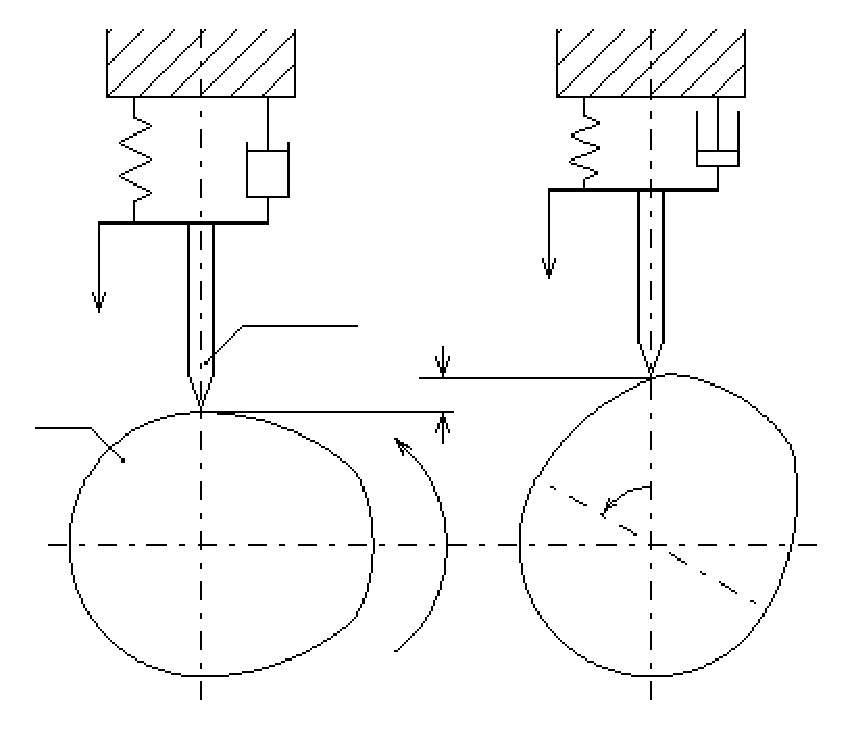
\includegraphics[height=8cm]{./Figures/cam}}}
 \put (0,52){\mbox{$F_{v}$}}
 \put (2,34.5){\mbox{\textit{Cam}}}
 \put (26,46){\mbox{\textit{Follower}}}
 \put (15,46){\mbox{\textit{$\mu$}}}
 \put (9,62){\mbox{$\kappa$}}
 \put (32,62){\mbox{$\zeta$}}
 \put (38,40){\mbox{$\delta c (\beta)$}}
 \put (66,28){\mbox{$\beta$}}
 \put (2.5,6){\mbox{\textit{$t=0$}}}
 \put (52.4,6){\mbox{\textit{$t=\beta$}}}
 \put (18.5,-1){\mbox{\textit{(a)}}}
 \put (69.4,-1){\mbox{\textit{(b)}}}
\end{picture}
\begin{picture}(90,80)(-3,0)
 \put (0,0){\mbox{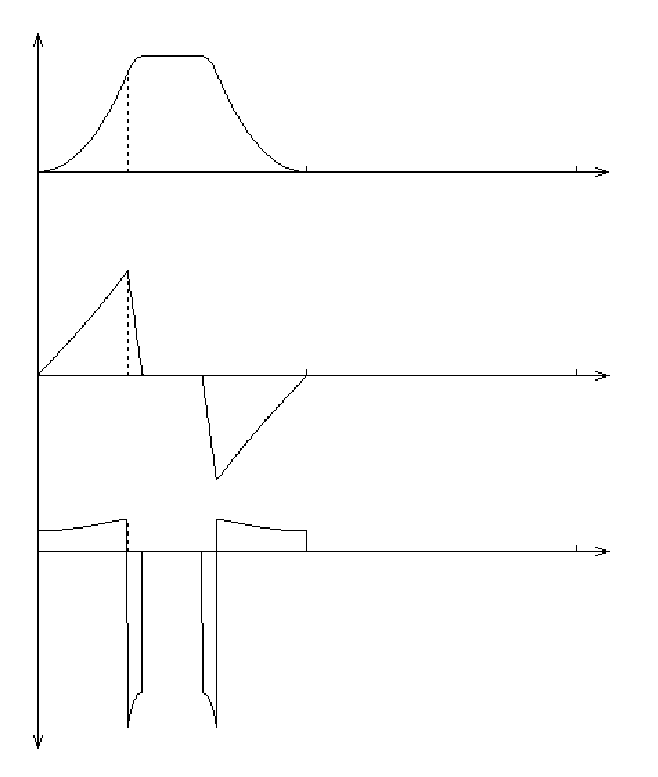
\includegraphics[height=8cm]{./Figures/campva}}}
 \put (-3,75){\mbox{$\delta c$}}
 \put (-3,49){\mbox{$ \frac{dc}{dt}$}}
 \put (-3,25){\mbox{$ \frac{d^2c}{dt^2}$}}
 \put (30,60){\mbox{$\pi$}} \put (58,60){\mbox{$2\pi$}}
 \put (10,60){\mbox{$\beta$}}
% \put (30,38){\mbox{$\pi$}} \put (58,38){\mbox{$2\pi$}}
% \put (9,38){\mbox{$\beta$}}
% \put (30,19){\mbox{$\pi$}} \put (58,19){\mbox{$2\pi$}}
% \put (9,19){\mbox{$\beta$}}
 \put (32,-1){\mbox{\textit{(c)}}}
\end{picture}
%\begin{picture}(45,20)(-90,-20)
% \put (3,10){\mbox{$v^{+}=(1+r)\frac{dc}{dt}-rv^{-}$}}
% \put (16,-1){\mbox{\textit{(d)}}}
%\end{picture}
%\begin{picture}(45,20)(-85,-20)
% \put (-2,20){\mbox{$k \hspace{4mm}= \hspace{1.5mm}5 \times 10^{4}\hspace{1.5mm} (N /m)$}}
% \put (-2,16){\mbox{$b \hspace{4mm}= \hspace{1.5mm}0 \hspace{10.5mm}(N\hspace{0.5mm} s/m)$}}
% \put (-2,12){\mbox{$F_{ext} \hspace{0.2mm}= \hspace{1.5mm}0 \hspace{12.5mm}(N)$}}
% \put (-2,8){\mbox{$c \hspace{4mm}\in \hspace{1.5mm}[0.52\hspace{2mm} 0.67]\hspace{2mm}(m)$}}
% \put (-2,4){\mbox{$r \hspace{4mm}= \hspace{1.5mm}0.9$}}
% \put (16,-1){\mbox{\textit{(e)}}}
%\end{picture}
  \caption{Cam-Shaft's schematics. \textit{(a)} t=0. \textit{(b)} t=$\beta$. \textit{(c)} Constraint position $\delta c(t)$, velocity $\frac{dc}{dt}(t)$ and acceleration $\frac{d^{2}c}{dt}(t^{2})$.}
  \label{Fig:cam-shaft}
\end{figure}
\subsection{The cam-follower as a Lagrangian NSDS.}
%\textit{\textbf{WP2 Template 1 Simulation of a bouncing ball with the Moreau's Time-Stepping scheme.}\\{Acary}}\\
 It is possible to completely describe the cam-follower system as a
 driven impact oscillator into the framework of \textit{Lagrangian NSDS} using a
translation in space. Setting $\hat u(t)=u(t)-c(t)$ and $\hat
v(t)= v(t)-dc/dt$, then equations (\ref{eq:sols}) and
(\ref{eq:il}) can be expressed as (the argument $t$ will not be
explicitly written)
\begin{eqnarray}
  \label{eq:trans}
  \mu\frac{d^2\hat u}{dt^2}+\zeta\frac{d\hat u}{dt}+\kappa
  \hat u=f_{v}-\left(\mu\frac{d^2c}{dt^2}+\zeta\frac{dc}{dt}+\kappa
  c\right)&\equiv &\hat f,  \; \text{\hspace{6.5mm} \text{if} \hspace{3mm}$\hat u >
 0$.}\\
\hat v^+&=&-r \hat v^- , \; \text{ \text{if}\hspace{3mm}$\hat
u=0$.}
\end{eqnarray}
Using the framework presented in [2] we have that the equation of
motion of a Lagrangian system may be stated as follows :
\begin{eqnarray}
  \label{eq:lag1}
  M(q)\ddot q + Q(q,\dot q) + F(\dot q, q , t) = F_{ext}(t) + R
\end{eqnarray}

From the (\ref{eq:trans}) we can derive all of the terms which
define a Lagrangian NSDS. In our case the model is completely
linear:
\begin{eqnarray}
  \nonumber
  q&=& \left[\begin{array}{c}  \hat u  \end{array}\right]    \\
  \nonumber
  M(q)&=&  \left[\begin{array}{c} \mu  \end{array}\right] \\
  \label{eq:lag2}
  Q(q,\dot q )& = &\left[\begin{array}{c} 0  \end{array}\right]  \\
  \nonumber
  F(q, \dot q ) &=&  \left[\begin{array}{c} \zeta \end{array}\right] \dot q +  \left[\begin{array}{c} \kappa  \end{array}\right] q\\
  \nonumber
  F_{ext}& = & \left[\begin{array}{c} \hat f \end{array}\right]
\end{eqnarray}

The unilateral constraint requires that:
\begin{eqnarray}
\label{eq:constr} \nonumber
 \hat u \geq 0
\end{eqnarray}
so we can obtain
\begin{eqnarray}
y &= & H^T q + b \\
\nonumber H^T &=&\left[\begin{array}{c} 1 \end{array}\right]\\
\nonumber b&=&0
\end{eqnarray}

In the same way, the reaction force due to the constraint is
written as follows:
\begin{eqnarray}
\nonumber R=H \lambda, \hspace{1cm}  \text{with }
H=\left[\begin{array}{c} 1
\end{array}\right]
\end{eqnarray}

The unilataral contact law may be formulated as follow:
\begin{eqnarray}
  \label{eq:119}
  0 \leq y \perp \lambda\geq 0
\end{eqnarray}
and the Newton's impact law:
\begin{eqnarray}
  \label{eq:120}
\text{If } y=0, \dot{y}^+ =-r\dot{y}^-
\end{eqnarray}

\subsection{Implementation in the platform}
%The code for the simulation of the Cam Follower system using the
%SICONOS software package is:
For the simulation of the cam follower system follow the steps

\begin{enumerate}
\item Move to the working directory \verb"sample/CamFollower"

\verb"$cd sample/CamFollower "

\item Clean the directory form binary files using the
\verb"siconos" command

\verb"$siconos -c "

\item Compile the file \verb"CamFollowerNoXml.cpp" in
the sample folder ({\em See} the code at the end of the section)

\verb"$siconos CamFollowerNoXml.cpp"

\item Change the simulation parameters ({\em i.e.}
Follower initial position and velocity, cam initial angle,
simulations time, cam rotational speed in rpm, etc.) in the file
\verb"CamFollowerNoXml.cpp".

\end{enumerate}

Next we present the sample code for the
\verb"CamFollowerNoXml.cpp" file:
\begin{tabbing}
\hspace{1cm}\= \hspace{0.5cm}\= \hspace{1cm}\= \hspace{1cm}\= \hspace{1cm}\\
 \> \+ int main(int argc, char* argv[]) {\bf \{} \\
 \>  {\bf\{} \+ \hspace{0.5cm}\= \hspace{2cm}\= \hspace{1cm}\=\hspace{1cm}\=\hspace{1cm}\=\hspace{1cm}\=\\
 \> \em   // ======== Creation of the model =============\\
 \> \em  // User-defined main parameters\\

 \> double rpm=358; \\
 \> double phi\_0=0;\\

 \> unsigned int dsNumber = 1; \>\>\>\> \em // the Follower and the ground\\
 \> unsigned int nDof = 1;  \>\>\>\>    \em // degrees of freedom for the Follower\\
 \> double t0 = 0;            \>\>\>\>  \em   // initial computation time\\
 \> double T = 5;             \>\>\>\>  \em    // final computation time\\
 \> double h = 0.0001;   \>\>\>\>       \em // time step\\
 \> int Kplot;\\
 \> Kplot=(int)(Tplot/h);\\

 \> double position\_init = 0.4;\>\>\>\> \em// initial position for lowest bead.\\
 \> double velocity\_init = 0.4;\>\>\>\> \em// initial velocity for lowest bead.\\
 \\
 \> \em    // ======= Dynamical systems =========\\
 \\
 \>     vector<DynamicalSystem *> vectorDS; // the list of DS\\
 \>     vectorDS.resize(dsNumber,NULL);\\
\\
 \> SiconosMatrix *Mass, *K, *C;        // mass/rigidity/viscosity\\
 \> Mass = new SiconosMatrix(nDof,nDof);\\
 \> (*Mass)(0,0) = 1.221;\\
 \> K = new SiconosMatrix(nDof,nDof);\\
 \> (*K)(0,0) = 1430.8;\\
 \> C = new SiconosMatrix(nDof,nDof);\\
 \> (*C)(0,0) = 0;\\
\\
 \>  //  Initial positions and velocities  \\
 \>  vector<SimpleVector *> position\_0;\\
 \>  vector<SimpleVector *> velocity\_0;\\
 \>  position\_0.resize(dsNumber,NULL);\\
 \>  velocity\_0.resize(dsNumber,NULL);\\
 \>  position\_0[0] = new SimpleVector(nDof);\\
 \>  velocity\_0[0] = new SimpleVector(nDof);\\
 \>  (*(position\_0[0]))(0) = position\_init;\\
 \>  (*(velocity\_0[0]))(0) = velocity\_init;\\
 \\
 \>  vectorDS[0] =\\ \>
 new LagrangianLinearTIDS(0,nDof,*(position\_0[0]),*(velocity\_0[0]),*Mass,*K,*C);\\
\\
 \> static\_cast<LagrangianDS*>(vectorDS[0])
 \\ \>\>\>->setComputeFExtFunction("FollowerPlugin.so", "FollowerFExt");\\
\\
 \> // Example to set a list of parameters in FExt function.\\
 \> // 1 - Create a simple vector that contains the required
 parameters.\\
\\
 \> // Here we set two parameters, the DS  number.\\
 \> SimpleVector * param = new SimpleVector(2);\\
\\
 \> (*param)(0)=rpm;\\
 \> (*param)(1)=phi\_0;\\
 \> // 2 - Assign this param to the function FExt\\
 \> static\_cast<LagrangianDS*>(vectorDS[0])->setParametersListPtr(param,2);\\
 \> // 2 corresponds to the position of FExt in the stl vector of possible parameters. \\
\> //  0 is mass, 1 FInt.\\ % and so on.\\
 \> // Now the cam rotational velocity in rpms will be available in FExt plugin.\\
\\
\> // ===== Interactions =====\\
\\
 \>  vector<Interaction*> interactionVector;\\
 \>  interactionVector.resize(1,NULL);\\
 \>  vector<DynamicalSystem*> *dsConcerned = \\ \>\>\> new vector<DynamicalSystem*>(dsNumber);\\
\\
 \>  // ===== Non Smooth Law =====\\
 \>  double e = 0.8;\\

 \>  // Interaction Follower-floor\\
 \>  SiconosMatrix *H = new SiconosMatrix(1,nDof);\\
 \>  (*H)(0,0) = 1.0;\\
 \>  NonSmoothLaw * nslaw = new NewtonImpactLawNSL(e);\\
 \>  Relation * relation = new LagrangianLinearR(*H);\\
 \>  (*dsConcerned)[0] = vectorDS[0];\\

 \>  interactionVector[0] = new Interaction("Follower-Ground",0,1, dsConcerned);\\
 \>  interactionVector[0]->setRelationPtr(relation);\\
 \>  interactionVector[0]->setNonSmoothLawPtr(nslaw);\\

 \> // ===== Interactions =====\\
\\
 \> // ===== NonSmoothDynamicalSystem =====\\

 \> bool isBVP =0;\\
 \> NonSmoothDynamicalSystem * nsds = \\
\>\>\>\> new NonSmoothDynamicalSystem(isBVP);\\
\\
 \>// Set DS of this NonSmoothDynamicalSystem\\
 \> nsds->setDynamicalSystems(vectorDS);       \\
 \> // Set interactions of the  NonSmoothDynamicalSystem\\
 \> nsds->setInteractions(interactionVector);  \\
\\
 \> // ===== Model =====\\
\\
 \> Model * Follower = new Model(t0,T);\\
 \> // set NonSmoothDynamicalSystem of this  model\\
 \> Follower->setNonSmoothDynamicalSystemPtr(nsds);\\
 \\
 \> // ====== Strategy ======\\
\\
 \> double theta = 0.5;  \>\>\>      // theta for Moreau integrator\\
 \> string solverName = "QP" ;\\
\\
 \> Strategy* S = new TimeStepping(Follower);\\
\\
 \> // -- Time discretisation --\\
 \> TimeDiscretisation * t = new TimeDiscretisation(h,S);\\
\\
 \> // -- OneStepIntegrators --\\
 \> vector<OneStepIntegrator *> vOSI;\\
 \> vOSI.resize(dsNumber,NULL);\\
 \> vOSI[0] = new Moreau(t,vectorDS[0],theta);\\
 \> S->setOneStepIntegrators(vOSI);\\
\\
 \> // -- OneStepNsProblem --\\
 \> OneStepNSProblem * osnspb = new LCP(S,solverName,101, 0.0001,"max",0.6);\\
 \> S->setOneStepNSProblemPtr(osnspb); // set OneStepNSProblem of the
 strategy\\
 \> cout << "=== End of model loading === " << endl;\\
 \> // ==== End of model definition======\\
\\
\\
\\
 \> // ========= Computation============\\
\\
 \> // --- Strategy initialization ---\\
 \> S->initialize();\\
 \> cout <<"End of strategy initialisation" << endl;\\
\\

 \> int k = t->getK(); \> \> \> \> // Current step\\
 \> int N = t->getNSteps(); \> \> \> \> // Number of time steps\\
\\
 \> // --- Get the values to be plotted ---\\
 \> // -> saved in a matrix dataPlot\\
 \> unsigned int outputSize = 8;\\
\\
 \> SiconosMatrix DataPlot(Kplot+1,outputSize );\\
 \>   // For the initial time step:\\
 \\
 \> // time\\
 \>     DataPlot(k,0) = k*t->getH();\\
 \\
 \>     DataPlot(k,1) = static\_cast<LagrangianDS*>(vectorDS[0])->getQ()(0);\\
 \>     DataPlot(k,2) = static\_cast<LagrangianDS*>(vectorDS[0])->getVelocity()(0);\\
 \>     DataPlot(k,3) = (Follower->getNonSmoothDynamicalSystemPtr()->\\
 \> \> getInteractionPtr(0)->getLambda(1))(0);\\
 \>     DataPlot(k,4) = static\_cast<LagrangianDS*>(vectorDS[0])->getFExt()(0);\\
 \\
 \>     // State of the Cam\\
 \>      double CamEqForce,CamPosition,CamVelocity,CamAcceleration;\\

 \>     CamEqForce=\\
 \> \> CamState(k*t->getH(),rpm,CamPosition,CamVelocity,CamAcceleration);\\
 \>     // Position of the Cam\\
 \>      DataPlot(k, 5) = CamPosition;\\
 \>      // Velocity of the Cam\\
 \>      DataPlot(k, 6) = CamVelocity;\\
 \>      // Acceleration of the Cam\\
 \>      DataPlot(k, 7) =\\
 \> \>CamPosition+static\_cast<LagrangianDS*>(vectorDS[0])->getQ()(0);\\
\\
 \> // --- Time loop ---\\
 \> cout << "Start computation ... " << endl;\\
 \> while(k < N)\\
 \>   {\bf \{ }\+ \hspace{0.5cm}\= \hspace{2cm}\= \hspace{1cm}\=\hspace{1cm}\=\hspace{1cm}\=\hspace{1cm}\=\\\\
 \> // --- Get values to be plotted ---\\
 \>     DataPlot(k,0) = k*t->getH();\\
 \\
 \>     DataPlot(k,1) = \\
 \> \> static\_cast<LagrangianDS*>(vectorDS[0])->getQ()(0);\\
 \>     DataPlot(k,2) =  \\
 \> \> static\_cast<LagrangianDS*>(vectorDS[0])->getVelocity()(0);\\
 \>     DataPlot(k,3) =  \\
 \> \> (Follower->getNonSmoothDynamicalSystemPtr()->\\
 \> \> getInteractionPtr(0)->getLambda(1))(0);\\
 \>     DataPlot(k,4) = static\_cast<LagrangianDS*>(vectorDS[0])->getFExt()(0);\\
 \\

 \>     CamEqForce=\\
 \>  CamState(k*t->getH(),rpm,CamPosition,CamVelocity,CamAcceleration);\\
 \\
 \>      DataPlot(k, 5) = CamPosition;\\
 \>      DataPlot(k, 6) = CamVelocity;\\
 \>      DataPlot(k, 7) = CamPosition+\\
 \> \> static\_cast<LagrangianDS*>(vectorDS[0])->getQ()(0);\\

 \> // transfer of state i+1 into state i and time
 incrementation\\
 \> S->nextStep();\\

 \> // get current time step\\
 \> k = t->getK();\\
 \> // solve ...\\
 \> S->computeFreeState();\\
 \> S->computeOneStepNSProblem();\\
 \> // update\\
 \> S->update();
 \-\\
 \>   {\bf \} }\\
\>    // --- Output files ---\\
 \> DataPlot.rawWrite("result.dat", "ascii");\\

 \> // --- Free memory ---\\
 \> delete osnspb;\\
 \> delete vOSI[0];\\
 \> delete t;\\
 \> delete S;\\
 \> delete Follower;\\
 \> delete nsds;\\
 \> delete interactionVector[0];\\
 \> delete relation;\\
 \> delete nslaw;\\
 \> delete H;\\
 \> delete dsConcerned;\\
 \> delete vectorDS[0];\\
 \> delete position\_0[0];\\
 \> delete velocity\_0[0];\\
 \> delete C;\\
 \> delete K;\\
 \> delete Mass;\\

    \-\\
 \>  {\bf\}}
\end{tabbing}
%\end{enumerate}
\newpage
\subsection{Simulation}
We have perform the simulation of the cam follower system for
different values of the cam rotational speed with the SICONOS
software package using a time-stepping numerical scheme with step
size ($h=1e^{-4}$) and an event-driven scheme with minimum step
size \linebreak ($h_{min}=1e^{-12}$). Fig.
\ref{Fig:time_comparison} and \ref{Fig:state_comparison} show the
time simulations for different values of the cam rotational speed
and Fig. \ref{Fig:attractor_comparison} show the chaotic attractor
at $rpm=660$ for impact and stroboscopic Poincar\`e sections.

\begin{figure}[hbtp]
\vspace{5mm} \setlength{\unitlength}{1mm}
\begin{picture}(60,60)(0,-7)
 \put (0,0){\mbox{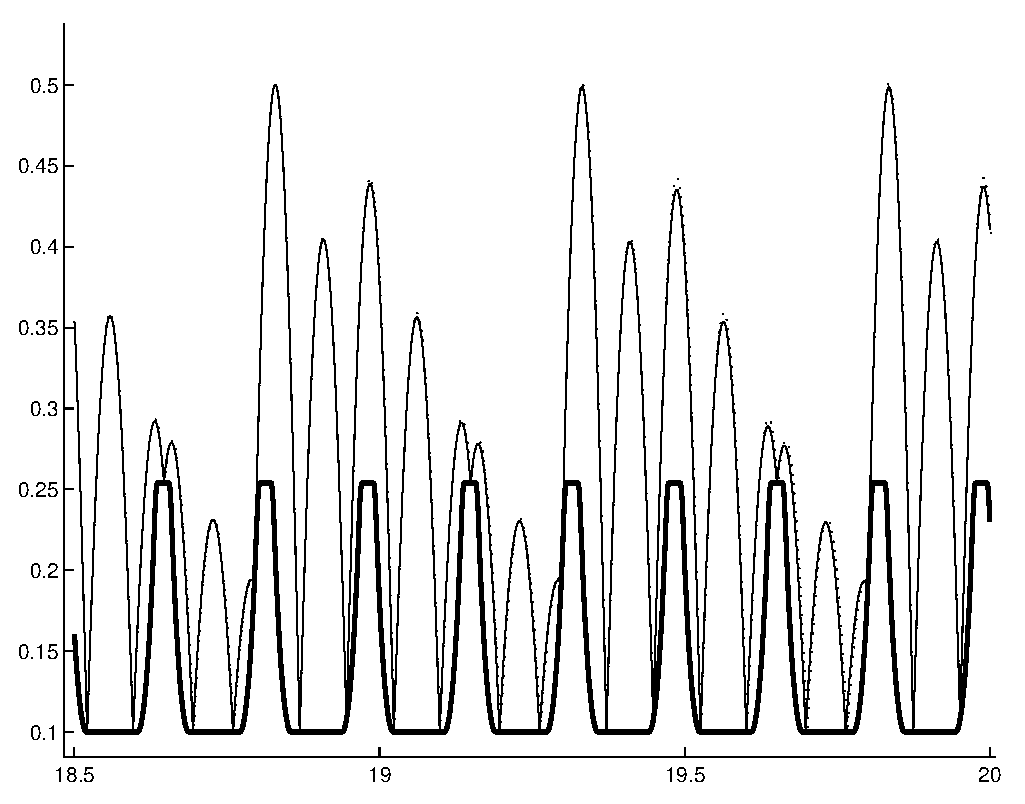
\includegraphics[height=6cm]{./comparison_figs/time_comparison_358}}}
  \put (35,-4){\mbox{\textit{(a)}}}
\end{picture}
\begin{picture}(60,60)(15,-7)
 \put (0,0){\mbox{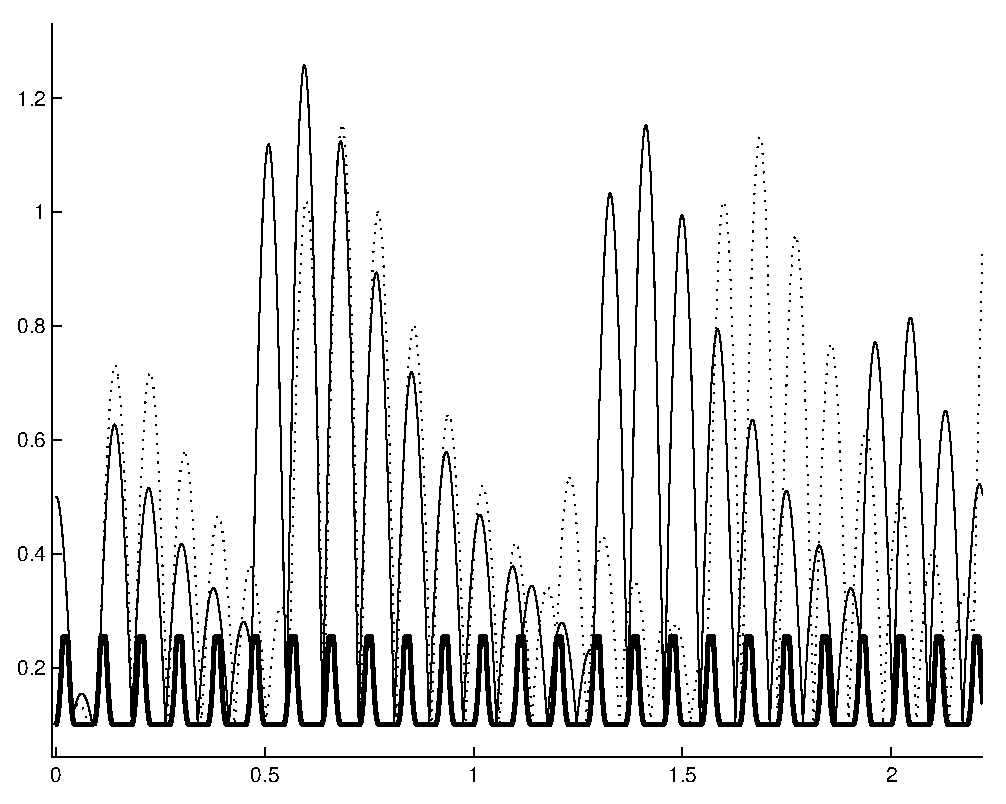
\includegraphics[height=6cm]{./comparison_figs/time_comparison_660}}}
 \put (35,-4){\mbox{\textit{(b)}}}
\end{picture}
\begin{picture}(60,60)(-40,-2)
 \put (0,0){\mbox{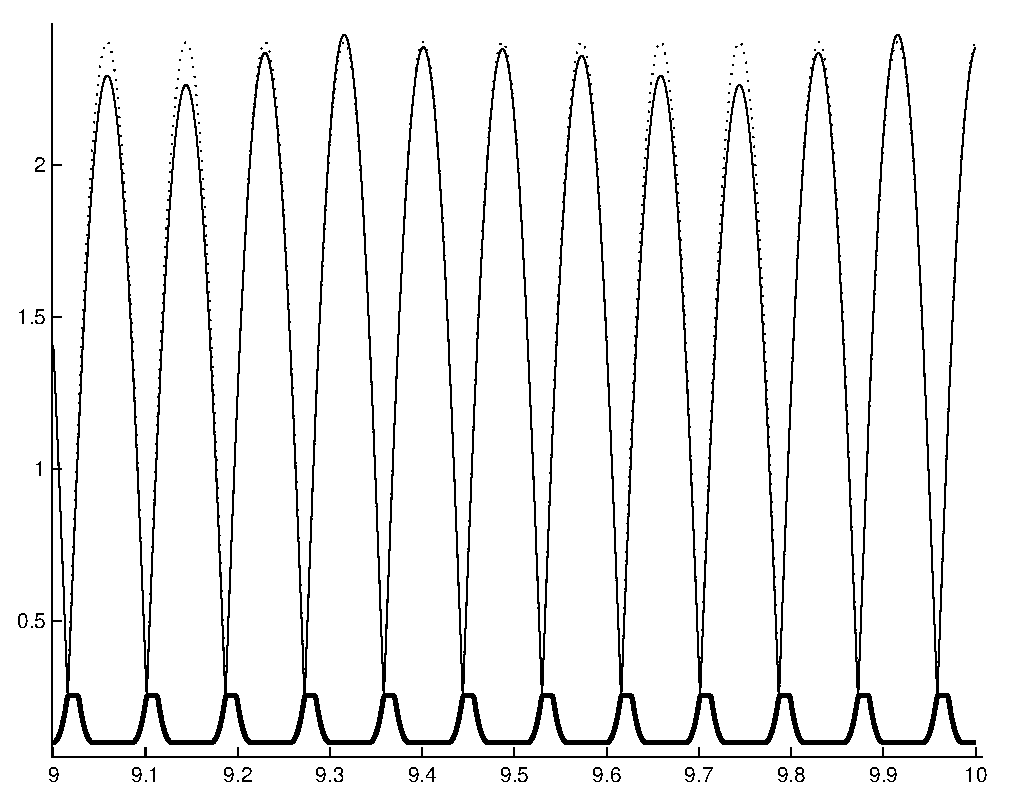
\includegraphics[height=6cm]{./comparison_figs/time_comparison_700}}}
 \put (35,-4){\mbox{\textit{(c)}}}
\end{picture}
  \caption{Time series using SICONOS platform. Time-stepping scheme (continuous line). Event-driven scheme (dashed line) \textit{(a)} rpm=358. \textit{(b)} rpm=660. \textit{(c)} rpm=700.}
  \label{Fig:time_comparison}
\end{figure}

\begin{figure}[hbtp]
\vspace{5mm} \setlength{\unitlength}{1mm}
\begin{picture}(60,60)(0,-7)
 \put (0,0){\mbox{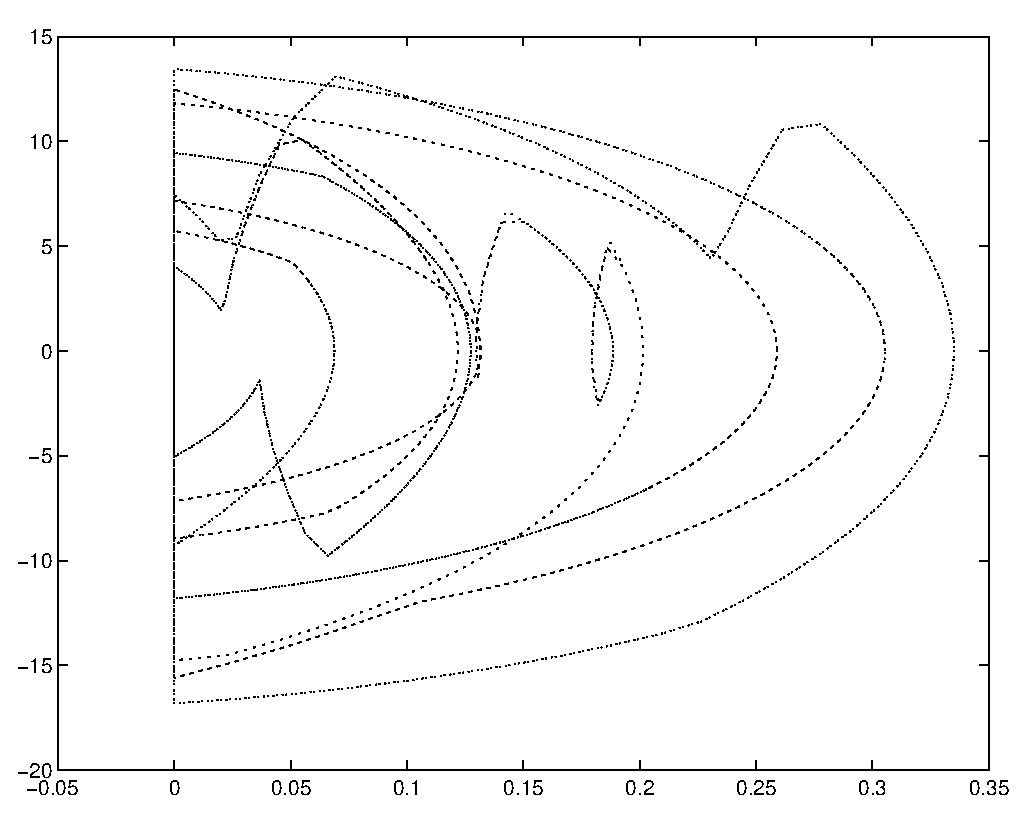
\includegraphics[height=6cm]{./comparison_figs/state_comparison_358event}}}
  \put (35,-4){\mbox{\textit{(a)}}}
\end{picture}
\begin{picture}(60,60)(15,-7)
 \put (0,0){\mbox{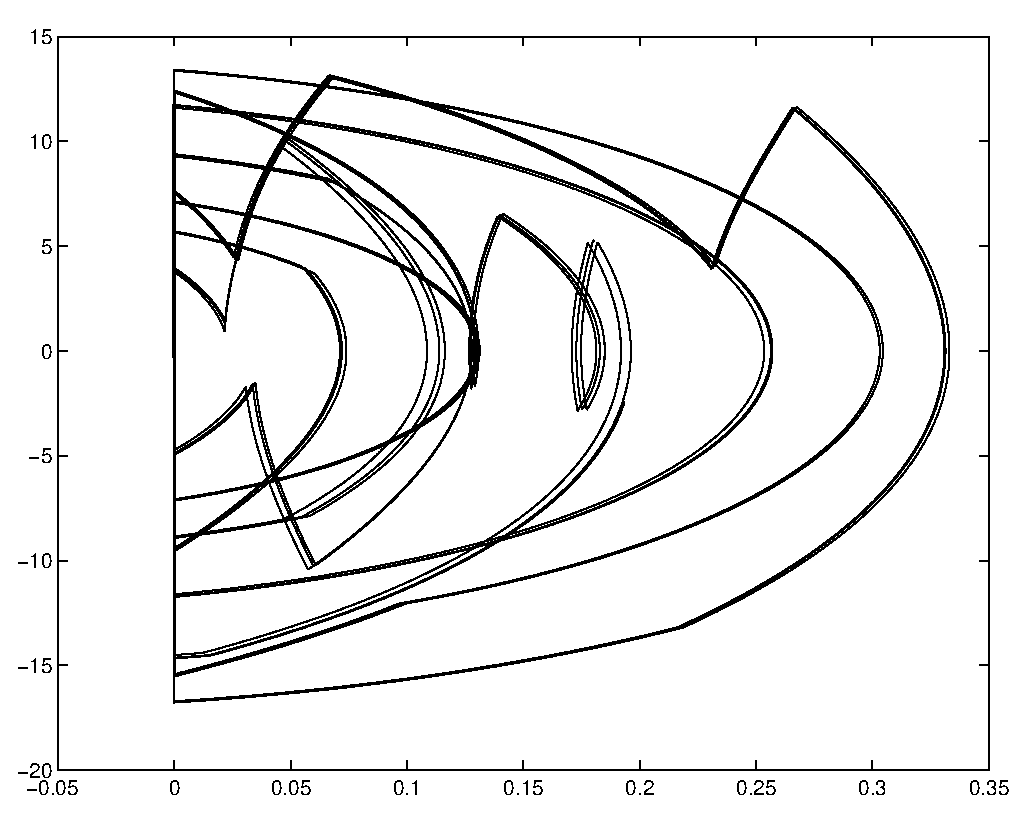
\includegraphics[height=6cm]{./comparison_figs/state_comparison_358siconos}}}
 \put (35,-4){\mbox{\textit{(b)}}}
\end{picture}
\begin{picture}(60,60)(0,-2)
 \put (0,0){\mbox{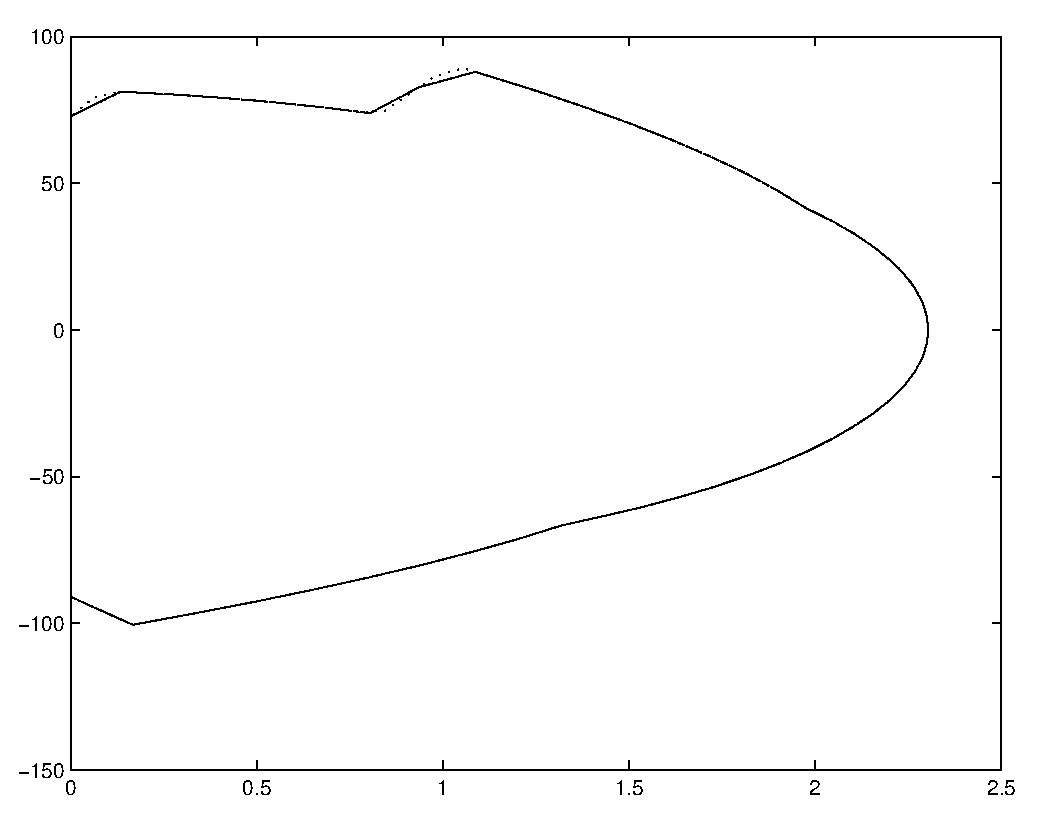
\includegraphics[height=6cm]{./comparison_figs/state_comparison_700event}}}
  \put (35,-4){\mbox{\textit{(c)}}}
\end{picture}
\begin{picture}(60,60)(-17,-2)
 \put (0,0){\mbox{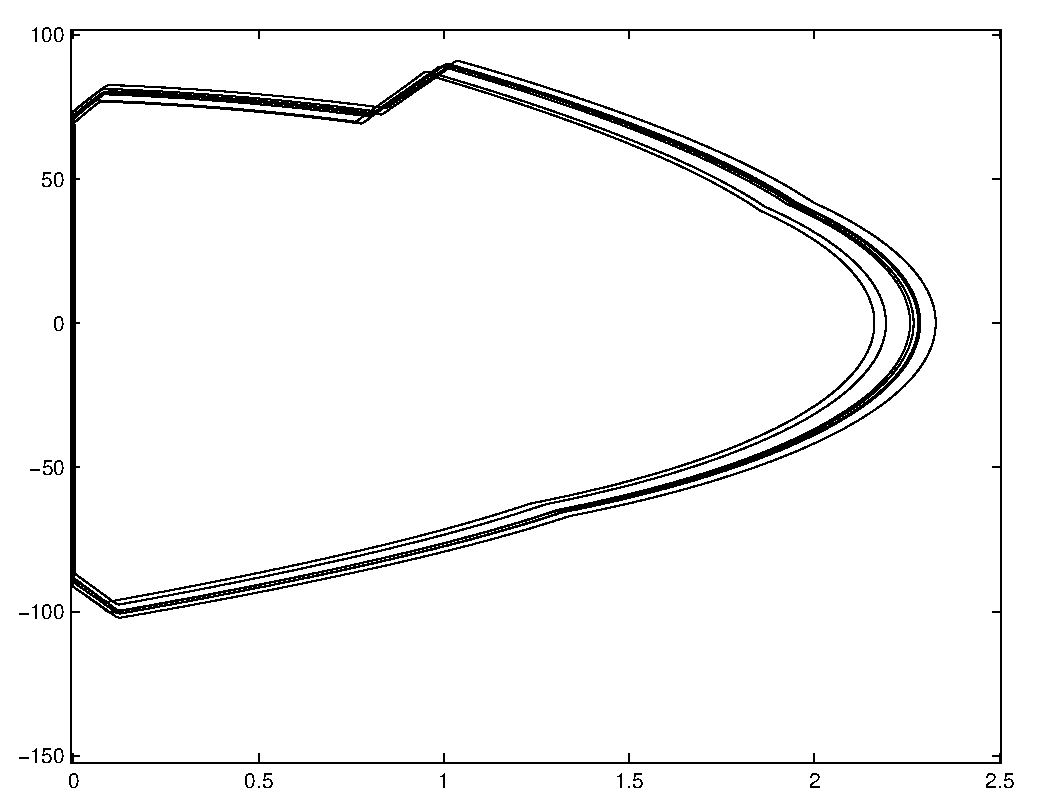
\includegraphics[height=6cm]{./comparison_figs/state_comparison_700siconos}}}
 \put (35,-4){\mbox{\textit{(d)}}}
\end{picture}
  \caption{State space comparison using SICONOS platform. \textit{(a)} rpm=358. Event Driven \textit{(b)} rpm=358. Time Stepping ($h=1e^{-4}$)\textit{(c)} rpm=700. Event Driven \textit{(d)} rpm=700. Time Stepping ($h=1e^{-4}$)}
  \label{Fig:state_comparison}
\end{figure}

\begin{figure}[hbtp]
\vspace{5mm} \setlength{\unitlength}{1mm}
\begin{picture}(60,60)(0,-7)
 \put (0,0){\mbox{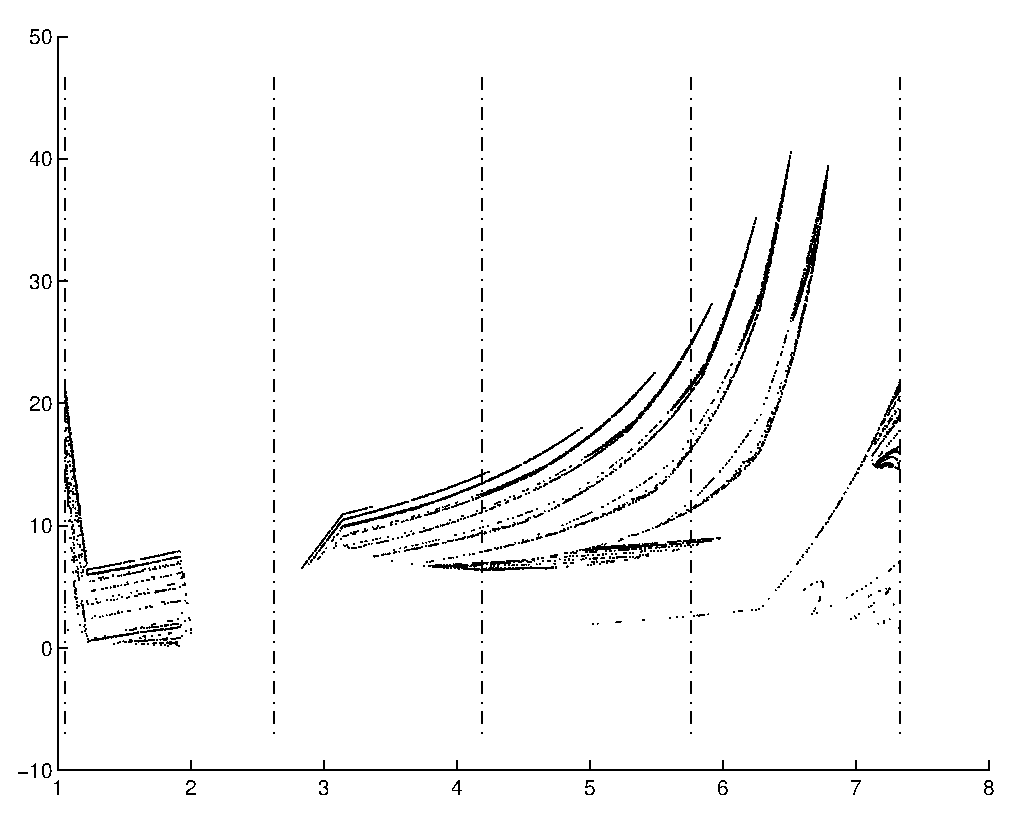
\includegraphics[height=6cm]{./comparison_figs/impact_map_660event}}}
  \put (35,-4){\mbox{\textit{(a)}}}
\end{picture}
\begin{picture}(60,60)(15,-7)
 \put (0,0){\mbox{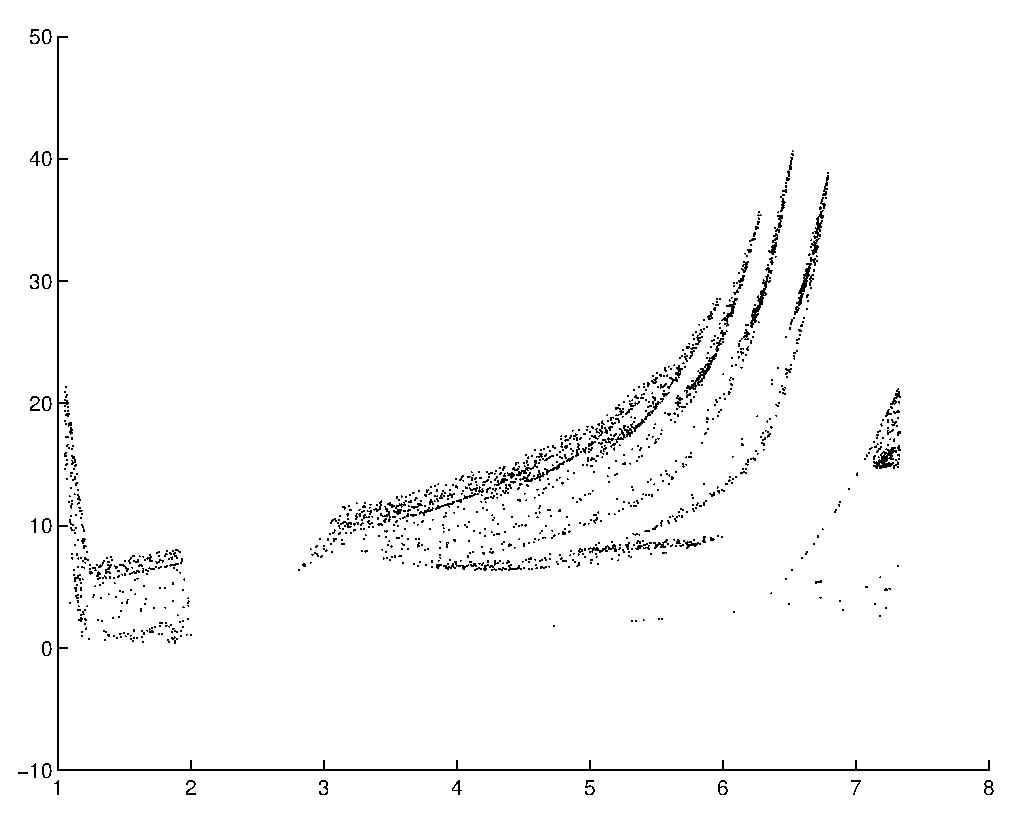
\includegraphics[height=6cm]{./comparison_figs/impact_map_660siconos}}}
 \put (35,-4){\mbox{\textit{(b)}}}
\end{picture}
\begin{picture}(60,60)(0,-2)
 \put (0,0){\mbox{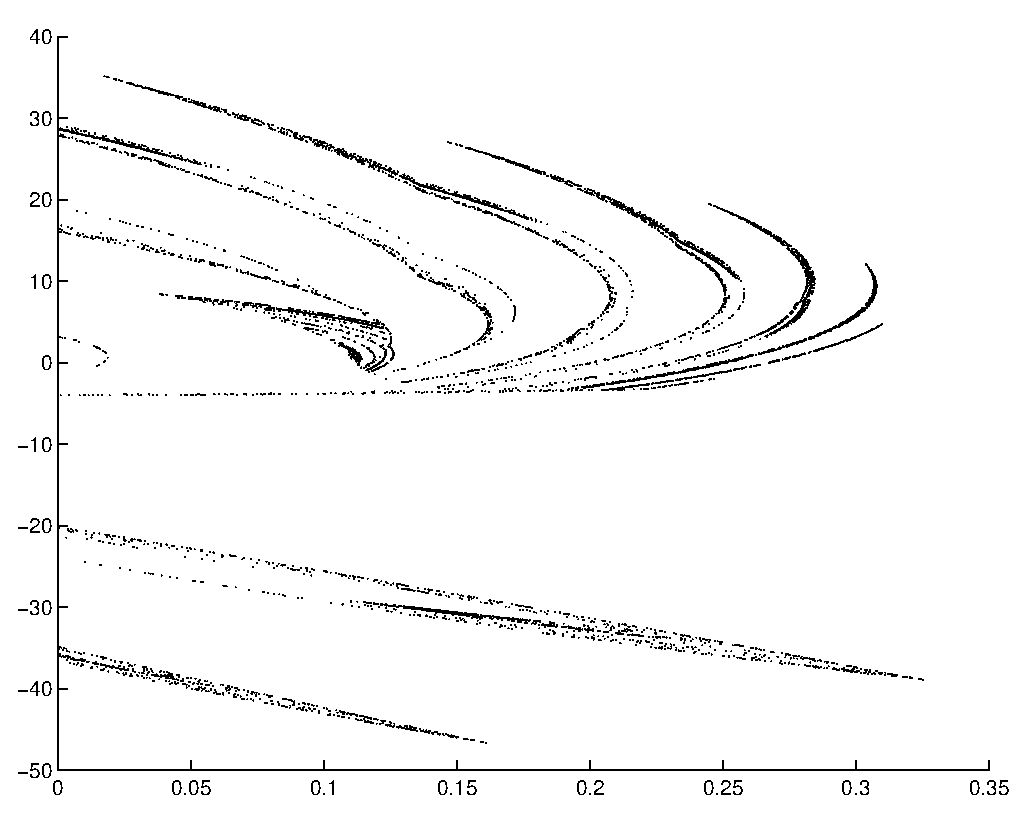
\includegraphics[height=6cm]{./comparison_figs/stroboscopic_map_660event}}}
  \put (35,-4){\mbox{\textit{(c)}}}
\end{picture}
\begin{picture}(60,60)(-17,-2)
 \put (0,0){\mbox{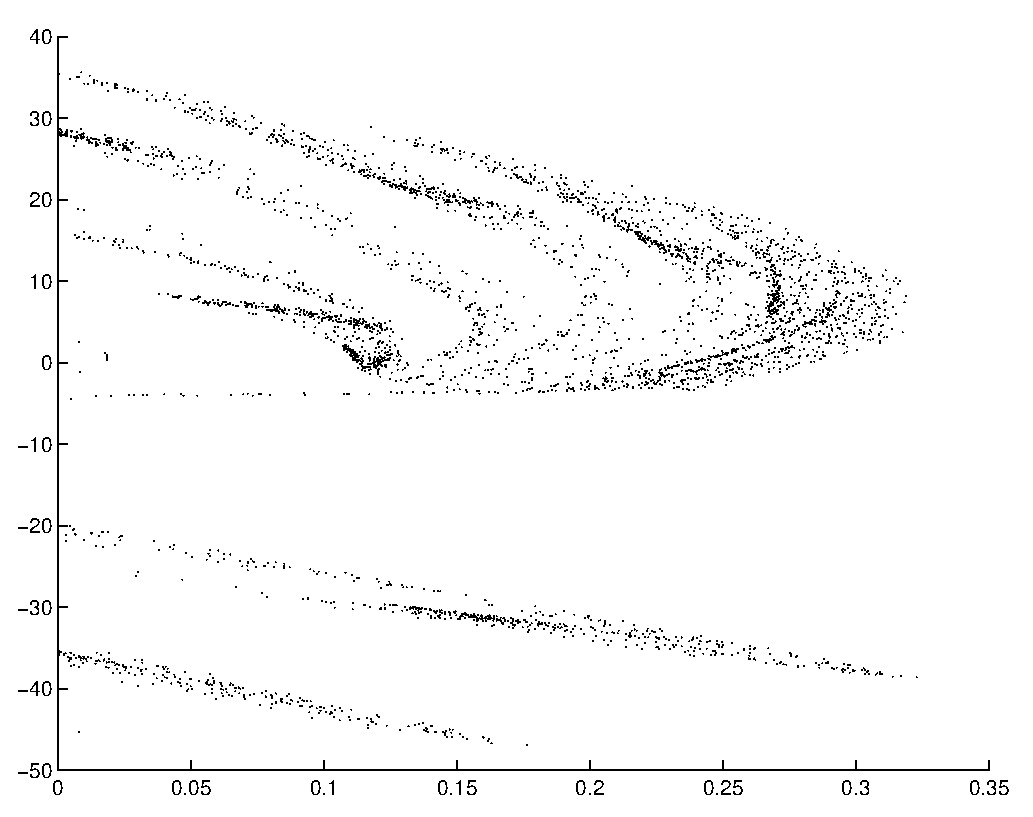
\includegraphics[height=6cm]{./comparison_figs/stroboscopic_map_660siconos}}}
 \put (35,-4){\mbox{\textit{(d)}}}
\end{picture}
  \caption{Attractors comparison using SICONOS platform at rpm=660. \textit{(a)}  Impact map. (Event Driven) \textit{(b)} Impact Map. Time Stepping ($h=1e^{-4}$)\textit{(a)}  Stroboscopic map. (Event Driven) \textit{(b)} Stroboscopic Map. Time Stepping ($h=1e^{-4}$)}
  \label{Fig:attractor_comparison}
\end{figure}

\chapter{Quartic Formulation}


\subsection{Slidding ?}
It consists in finding $\alpha >0$ and $R \in \partial K_{\mu}$ such that $-\alpha \left(\begin{array}{l} 0\\ R_T\end{array}\right)=MR+q$. That is :
  \begin{equation}
\label{eq_quartic1}
\left[\begin{array}{c}
M+ \left(\begin{array}{ccc} 0&0&0\\ 0&\alpha&0 \\ 0&0&\alpha \end{array}\right)
\end{array}\right]R+q=0
\end{equation}

  \subsubsection{$R_T$ is on a conic}
  The first line of the system~\ref{eq_quartic1} and the $R \in \partial K_{\mu}$ is the intersection between a plan and a cone in $\mathbb{R}^3$, endeed:
  \begin{equation}
\label{eq_quartic2}
\begin{array}{l}
 \mu R_N =  \parallel R_T \parallel  \\
\frac{M_{11}}{\mu} \parallel R_T \parallel = -q_1-M_{12}R_{T1}-M_{13}R_{T2}
\end{array}
\end{equation}
That is:
\begin{equation}
\label{eq_quartic2}
\begin{array}{l}
\mu^2 R_N^2 =  (R_{T1}^2 +R_{T1}^2)  \\
\frac{M_{11}^2}{\mu^2} (R_{T1}^2 +R_{T1}^2)=(-q_1-M_{12}R_{T1}-M_{13}R_{T2})^2
\end{array}
\end{equation}
That means that $R_T$ is contained in a conic,  focus and directrice are:
\begin{equation}
\label{eq_quartic3}
\begin{array}{l}
\mathcal{D} : q_1+M_{12}R_{T1}+M_{13}R_{T2} =0  \\
focus : \mathcal{O}\\
\frac{M_{11}^2}{\mu^2}  Dist(\mathcal{O}, R_T) ^2=Dist(\mathcal{D},R_T)^2 (M_{12}^2+M_{13}^2)\\
\frac{Dist(\mathcal{O}, R_T)}{Dist(\mathcal{D},R_T)}=\frac{\mu\sqrt{(M_{12}^2+M_{13}^2)}}{M_{11} }=e
\end{array}
\end{equation}
The parametric equation is:
\begin{equation}
\label{eq_quartic4}
\begin{array}{l}
R_{T1}=r cos(\theta )\\
R_{T2}=r sin(\theta )\\
r=\frac{p}{1+ecos(\theta - \phi)}
\end{array}
\end{equation}
With $p$ an simple expression of $M_{11},M_{12},M_{13}$, and $\phi$ a constant angle between $\mathcal{D}$ and $(O,R_{T1})$
\subsubsection{The two last line of the system~\ref{eq_quartic1}}
\begin{equation}
\label{eq_quartic5}
\frac{\parallel R_T \parallel}{\mu} \tilde M_{1.} +\left(\tilde M+\left(\begin{array}{cc} \alpha&0 \\ 0&\alpha \end{array}\right)\right)R_T+\tilde q=0
\end{equation}
$\tilde M$ is symetric, so it exists a unitary matrix $V$ such that $V \tilde M V^T = \left(\begin{array}{cc} d_1&0 \\ 0&d_2 \end{array}\right)$.  One can get:
\begin{equation}
\label{eq_quartic6}
\frac{\parallel R_T \parallel}{\mu} V \tilde M_{1.} +V \left(\tilde M+\left(\begin{array}{cc} \alpha&0 \\ 0&\alpha \end{array}\right)\right)V^TVR_T+V\tilde q=0
\end{equation}
Rename:
\begin{equation}
\label{eq_quartic7}
  \frac{\parallel \bar R_T \parallel}{\mu} \bar M_{1.} +\left(\begin{array}{cc} d_1+\alpha&0 \\ 0&d_2+\alpha \end{array}\right)\overline R_T+\bar q=0
  \end{equation}
In the plan, either $V$ is a rotation or a symetrie. So $ \bar R_T=VR_T$ is a conic with the same focus and a rotated directrice, it means that it exists $\phi_1$ such that :

\begin{equation}
\label{eq_quartic8}
\begin{array}{l}
\bar R_{T1}=r cos(\theta )\\
\bar R_{T2}=r sin(\theta )\\
r=\frac{p}{1+ecos(\theta - \phi_1)}
\end{array}
\end{equation}
The equation~\ref{eq_quartic7} is :
\begin{equation}
\label{eq_quartic9}
\begin{array}{l}
  (d_1+\alpha)\bar R_{T1}=-\bar q_1+a_1 \parallel R_T \parallel\\
(d_2+\alpha)\bar R_{T2}=-\bar q_2+a_2 \parallel R_T \parallel
\end{array}
\end{equation}
The case ($\bar R_{T1} = 0$ or  $\bar R_{T2} = 0$) has to be examine. We try to eliminate $alpha$:
\begin{equation}
\label{eq_quartic10}
  \begin{array}{l}
    d_1 \bar R_{T1} \bar R_{T2}+\alpha \bar R_{T1} \bar R_{T2} =-\bar q_1\bar R_{T2}+a_1 \bar R_{T2} \parallel R_T \parallel\\
d_2 \bar R_{T1} \bar R_{T2}+\alpha \bar R_{T1} \bar R_{T2} =-\bar q_2\bar R_{T1}+a_2 \bar R_{T1} \parallel R_T \parallel
\end{array}
\end{equation}
that leads to:
\begin{equation}
\label{eq_quartic10}
  (d_1-d_2) \bar R_{T1} \bar R_{T2}=-\bar q_1\bar R_{T2}+\bar q_2\bar R_{T1}+(a_1 \bar R_{T2}-a_2 \bar R_{T1}) \parallel R_T \parallel\\
\end{equation}
The parametric expression of $\bar R_T$ leads to:
\begin{equation}
\label{eq_quartic11}
\begin{array}{l}
  (d_1-d_2)r^2cos(\theta )sin(\theta )=-\bar q_1rsin(\theta )+\bar q_2rcos(\theta )+r(a_1 rsin(\theta )-a_2 rcos(\theta )) \\
  \textrm{ie:}(d_1-d_2)rcos(\theta )sin(\theta )=-\bar q_1sin(\theta )+\bar q_2cos(\theta )+r(a_1 sin(\theta )-a_2 cos(\theta ))\\
  \end{array}
\end{equation}
with the expression of r:
\begin{equation}
\label{eq_quartic12}
\begin{array}{l}
(d_1-d_2)\frac{p}{1+ecos(\theta - \phi_1)}cos(\theta )sin(\theta )=\\-\bar q_1sin(\theta )+\bar q_2cos(\theta )+\frac{p}{1+ecos(\theta - \phi_1)}(a_1  sin(\theta )-a_2 cos(\theta ))\\\\
\textrm{ie:}(d_1-d_2)pcos(\theta )sin(\theta )=\\(1+ecos(\theta - \phi_1))(-\bar q_1sin(\theta )+\bar q_2cos(\theta ))+p(a_1  sin(\theta )-a_2 cos(\theta ))\\\\
\textrm{ie:}(d_1-d_2)pcos(\theta )sin(\theta )=\\(1+e(cos(\theta)cos(\phi_1)+sin(\theta)sin(\phi_1)))(-\bar q_1sin(\theta )+\bar q_2cos(\theta ))+p(a_1  sin(\theta )-a_2 cos(\theta ))\\\\
\textrm{ie:}(d_1-d_2)pcos(\theta )sin(\theta )+\\(1+ecos(\theta)cos(\phi_1)+esin(\theta)sin(\phi_1))(\bar q_1sin(\theta )-\bar q_2cos(\theta ))+p(-a_1  sin(\theta )+a_2 cos(\theta ))=0
 \end{array}
\end{equation}
rename :
\begin{equation}
\label{eq_quartic13}
\begin{array}{l}
Acos(\theta )^2+Bsin(\theta)^2+Csin(\theta )cos(\theta )+Dsin(\theta )+Ecos(\theta )=0
 \end{array}
\end{equation}
with
\begin{equation}
\label{eq_quartic12}
\begin{array}{l}
A=- e\bar q_2cos(\phi_1)\\
B=e \bar q_1sin(\phi_1)\\
C=(d_1-d_2)p+ecos(\phi_1)\bar q_1-esin(\phi_1)\bar q_2\\
D=\bar q_1-pa_1\\
E=-\bar q_2+pa_2\\
\end{array}
\end{equation}
rename :
Using the following set of unknown :
\begin{equation}
\label{eq_quartic14}
\begin{array}{l}
t=tan(\theta /2)\\
sin(\theta )=\frac{2t}{1+t^2}\\
cos(\theta )=\frac{1-t^2}{1+t^2}
 \end{array}
\end{equation}
leads to:
\begin{equation}
\label{eq_quartic13}
\begin{array}{l}
  A\frac{(1-t^2)^2}{1+t^2} +B\frac{4t^2}{1+t^2}+ C\frac{2t(1-t^2)}{1+t^2}+D2t+E(1-t^2)=0\\
\textrm{ie:}A(1-t^2)^2 + 4Bt^2+C2t(1-t^2)+2Dt(1+t^2)+E(1-t^2)(1+t^2)=0\\\\
\textrm{ie:}P_4=A-E\qquad P_3=-2C+2D \qquad P_2=4B-2A \qquad P_1=2C+2D \qquad P_0=A+E
 \end{array}
\end{equation}
Finally, we get 4 possible values for $R_T$, checking the sign of $\alpha$ and $R_N$ selects the solutions.

\subsubsection{case $R_{T12}=0$}
From~\ref{eq_quartic9}, $R_{T1}$ leads to:
\begin{equation}
\label{eq_quartic14}
\begin{array}{l}
  \parallel R_T \parallel=|\bar R_{T2}|=\frac{\bar q_1}{a_1}\\\\
  \bar R_T=\left(\begin{array}{c} 0 \\ \pm \frac{\bar q_1}{a_1} \end{array}\right)
 \end{array}
\end{equation}

From~\ref{eq_quartic9}, $R_{T2}$ leads to:
\begin{equation}
\label{eq_quartic14}
\begin{array}{l}
  \parallel R_T \parallel=|\bar R_{T1}|=\frac{\bar q_2}{a_2}\\\\
  \bar R_T=\left(\begin{array}{c}  \pm \frac{\bar q_2}{a_2} \\ 0 \end{array}\right)
 \end{array}
\end{equation}

From $\bar R_T$, we have to check the coherence with the equation~\ref{eq_quartic8}. If it is on the conic,  we compute R, and the sign condition of the equation~\ref{eq_quartic1} must be check.



\chapter{Alart--Curnier Formulation}

\section{Reduced formulation to local variables.}

\subsection{Formulation}

Let us start with 
\begin{equation}
  \label{eq:AC-L7}
  \begin{array}{l}
  \varPhi_1(U,P) =  - U_{k+1}  + \widehat W P_{k+1}  + U_{\mathrm{free}}\\ \\
  \varPhi_2(U,P) =  P_{\n} - \proj_{\nbR^{a}_+} (P_{\n} - \rho_{\n}\circ (U_{\n} +e \circ  U_{\n,k}) ) \\ \\
  \varPhi_3(U,P) =  P_{\t} - \proj_{\widehat {\bf D}(P_{\n},U_{\n})} (P_{{\t}} - \rho_{\t}\circ \,U_{\t} )
\end{array}
\end{equation}
where the modified friction disk for a contact $\alpha$ is
\begin{equation}\label{eq:AC-L3}
  \widehat {\bf D}^\alpha(P^\alpha_{\n,k+1},U_{\n,k+1}^{\alpha}) = {\bf D}(\mu(\proj_{\nbR_+} (P^\alpha_{\n,k+1} - \rho^\alpha_{\n}\,(U_{\n,k+1}^{\alpha}+e^\alpha U_{\n,k}^{\alpha}) )).
\end{equation}
\subsection{Structure of the Jacobians}

Let us denote the one element of the  generalized Jacobian by  $ H(U,P) \in \partial \Phi(U,P)$ which has the structure
\begin{equation}
  \label{eq:AC-L6}
   H(U,P) = 
   \left[\begin{array}{cccc}
       - I & 0 &  \widehat W_{\n\n} & \widehat W_{\n\t} \\ \\
       0  & -I  &  \widehat W_{\t\n} & \widehat W_{\t\t} \\ \\
       \partial_{U_{\n}} \Phi_2(U,P) & 0 &   \partial_{P_{\n}} \Phi_2(U,P) & 0 \\ \\
       \partial_{U_{\n}} \Phi_3(U,P) &  \partial_{U_{\t}} \Phi_3(U,P) &  \partial_{P_{\n}} \Phi_3(U,P)  & \partial_{P_{\t}} \Phi_3(U,P)
   \end{array}\right]
\end{equation}


\subsection{Computation of the gradients}


Let us consider the single contact case.
\paragraph{Computation of the gradients of $\Phi_2$}
\begin{equation}
  \label{eq:AC-T1}
  \begin{array}{l}
  \varPhi_2(U,P) =  P_{\n} - \proj_{\nbR^{a}_+} (P_{\n} - \rho_{\n} (U_{\n} +e  U_{\n,k}) ) \\ \\
\end{array}
\end{equation}
\begin{itemize}
\item \textbf{If} $P_{\n} - \rho_{\n} (U_{\n} +e  U_{\n,k}) \geq 0 $, we get 
  \begin{equation}
    \label{eq:AC-T2}
    \begin{array}{l}
      \varPhi_2(U,P) =  + \rho_{\n} (U_{\n} +e  U_{\n,k})
    \end{array}
  \end{equation}
  and 
  \begin{equation}
    \label{eq:AC-T3}
    \begin{array}{l}
     \partial_{U_{\n}} \varPhi_2(U,P) =  + \rho_{\n} \\ \\
     \partial_{P_{\n}} \varPhi_2(U,P) =  0 \\ \\ 
    \end{array}
  \end{equation}
\item \textbf{If} $P_{\n} - \rho_{\n} (U_{\n} +e  U_{\n,k})  < 0 $, we get 
  \begin{equation}
    \label{eq:AC-T4}
    \begin{array}{l}
      \varPhi_2(U,P) =  P_{\n}
    \end{array}
  \end{equation}
  and 
  \begin{equation}
    \label{eq:AC-T5}
    \begin{array}{l}
     \partial_{U_{\n}} \varPhi_2(U,P) =  0 \\ \\
     \partial_{P_{\n}} \varPhi_2(U,P) =  1 \\ \\ 
    \end{array}
  \end{equation}
\end{itemize}
\paragraph{Computation of the gradients of $\Phi_3$}
\begin{equation}
  \label{eq:AC-TT1}
  \begin{array}{l}
  \varPhi_3(U,P) =  P_{\t} - \proj_{\widehat {\bf D}(P_{\n},U_{\n})} (P_{\t} - \rho_{\t} U_{\t} ) \\ \\
\end{array}
\end{equation}
\begin{itemize}
\item \textbf{If} $\|P_{\t} - \rho_{\t} U_{\t}\| \leq \mu \max (0 ,P_{\n} - \rho_{\n} (U_{\n} +e  U_{\n,k}) ) $  , we get 
\begin{equation}
  \label{eq:AC-TT2}
  \begin{array}{l}
  \varPhi_3(U,P) =  + \rho_{\t} U_{\t} 
\end{array}
\end{equation}
and
 \begin{equation}
    \label{eq:AC-TT3}
    \begin{array}{l}
     \partial_{U_{\n}} \varPhi_3(U,P) =  0 \\ \\
     \partial_{P_{\n}} \varPhi_3(U,P) =  0 \\ \\ 
     \partial_{U_{\t}} \varPhi_3(U,P) =  + \rho_{\t} \\ \\
     \partial_{P_{\t}} \varPhi_3(U,P) =  0 \\ \\ 
    \end{array}
  \end{equation}
\item \textbf{If} $\|P_{\t} - \rho_{\t} U_{\t}\| > \mu \max (0 ,P_{\n} - \rho_{\n} (U_{\n} +e  U_{\n,k}) ) $  , we get 
\begin{equation}
  \label{eq:AC-TT4}
  \begin{array}{l}
  \varPhi_3(U,P) =  P_{\t} - \mu \max(0,P_{\n} - \rho_{\n} (U_{\n} +e  U_{\n,k}) )  \Frac{P_{\t} - \rho_{\t} U_{\t} }{ \| P_{\t} - \rho_{\t} U_{\t}\| }
\end{array}
\end{equation}

\begin{itemize}
\item  \textbf{If} $P_{\n} - \rho_{\n} (U_{\n} +e  U_{\n,k}) \leq 0$, we get 
  \begin{equation}
  \label{eq:AC-TT5}
  \begin{array}{l}
  \varPhi_3(U,P) =   P_{\t}
\end{array}
\end{equation}
and 
 \begin{equation}
   \label{eq:AC-TT6}
   \begin{array}{l}
     \partial_{U_{\n}} \varPhi_3(U,P) =  0 \\ \\
     \partial_{P_{\n}} \varPhi_3(U,P) =  0 \\ \\ 
     \partial_{U_{\t}} \varPhi_3(U,P) =  0 \\ \\
     \partial_{P_{\t}} \varPhi_3(U,P) =  I_2 \\ \\ 
   \end{array}
 \end{equation}
\item  \textbf{If} $P_{\n} - \rho_{\n} (U_{\n} +e  U_{\n,k}) > 0$, we get 
\begin{equation}
  \label{eq:AC-TT7}
  \begin{array}{l}
  \varPhi_3(U,P) =  P_{\t} - \mu (P_{\n} - \rho_{\n} (U_{\n} +e  U_{\n,k}) )  \Frac{P_{\t} - \rho_{\t} U_{\t} }{ \| P_{\t} - \rho_{\t} U_{\t}\| }
\end{array}
\end{equation}
and 
 \begin{equation}
   \label{eq:AC-TT8}
   \begin{array}{l}
     \partial_{U_{\n}} \varPhi_3(U,P) =  \mu \rho_{\n}  \Frac{P_{\t} - \rho_{\t} U_{\t} }{ \| P_{\t} - \rho_{\t} U_{\t}\| }\text{{\bf WARNING} case was not taken into account}\\ \\
     \partial_{P_{\n}} \varPhi_3(U,P) =  -\mu  \Frac{P_{\t} - \rho_{\t} U_{\t} }{ \| P_{\t} - \rho_{\t} U_{\t}\| } \\ \\ 
     \partial_{U_{\t}} \varPhi_3(U,P) =  \mu\rho_{\t}(P_{\n} - \rho_{\n} (U_{\n} +e  U_{\n,k}) ) \Gamma(P_{\t} - \rho_{\t} U_{\t})  \\ \\
     \partial_{P_{\t}} \varPhi_3(U,P) =  I_2-\mu(P_{\n} - \rho_{\n} (U_{\n} +e  U_{\n,k}) ) \Gamma(P_{\t} - \rho_{\t} U_{\t})  \\ \\ 
   \end{array}
 \end{equation}
\end{itemize}



\end{itemize}

\subsection{Rearranging the cases}

{\bf TO BE COMPLETED}
\section{Formulation with global variables.}

\subsection{Formulation}
Let us start with 
\begin{equation}
  \label{eq:GAC-L1}
  \begin{array}{l}
  \Psi_{1}^{a}(v,U,P) =  - \widehat M v_{k+1}  +  H P_{k+1}  + q \\ \\
  \Psi_{1}^{b}(v,U,P) =  - U_{k+1}  + H^\top v _{k+1}  + b \\ \\
  \Psi_2(v,U,P) =  P_{\n} - \proj_{\nbR^{a}_+} (P_{\n} - \rho_{\n}\circ (U_{\n} +e \circ  U_{\n,k}) ) \\ \\
  \Psi_3(v,U,P) =  P_{\t} - \proj_{\widehat {\bf D}(P_{\n},U_{\n})} (P_{{\t}} - \rho_{\t}\circ \,U_{\t} )
\end{array}
\end{equation}
where the modified friction disk for a contact $\alpha$ is
\begin{equation}\label{eq:GAC-L2}
  \widehat {\bf D}^\alpha(P^\alpha_{\n,k+1},U_{\n,k+1}^{\alpha}) = {\bf D}(\mu(\proj_{\nbR_+} (P^\alpha_{\n,k+1} - \rho^\alpha_{\n}\,(U_{\n,k+1}^{\alpha}+e^\alpha U_{\n,k}^{\alpha}) )).
\end{equation}

\subsection{Structure of the Jacobians}

 Let us denote the one element of the  generalized Jacobian by  $ H(v,U,P) \in \partial \Psi(s,U,P)$ which has the structure
\begin{equation}
  \label{eq:GAC-L3}
   H(v,U,P) = 
   \left[\begin{array}{ccccc}
       - \widehat M & 0 & 0 & H_{\n} & H_{\t} \\ \\
        H_{\n}^\top &  - I & 0 & 0 &0 \\ \\
        H_{\t}^\top &  0  & -I & 0 &0 \\ \\
        0 & \partial_{U_{\n}} \Psi_2(v,U,P) & 0 &   \partial_{P_{\n}} \Psi_2(v,U,P) & 0 \\ \\
        0 & \partial_{U_{\n}} \Psi_3(v,U,P) &  \partial_{U_{\t}} \Psi_3(v,U,P) &  \partial_{P_{\n}} \Psi_3(v,U,P)  & \partial_{P_{\t}} \Psi_3(v,U,P)
   \end{array}\right]
\end{equation}

We clearly have
\begin{equation}
  \label{eq:equivalentJacobian}
  \begin{array}{lcl}
     \partial_{U} \Psi_2(v,U,P) &=& \partial_{U} \Phi_2(U,P) \\ 
     \partial_{P} \Psi_2(v,U,P) &=& \partial_{P} \Phi_2(U,P) \\     
     \partial_{U} \Psi_3(v,U,P) &=& \partial_{U} \Phi_3(U,P) \\ 
     \partial_{P} \Psi_3(v,U,P) &=& \partial_{P} \Phi_3(U,P) \\
  \end{array}
\end{equation}
and we get
\begin{equation}
  \label{eq:GAC-L4}
   H(v,U,P) = 
   \left[\begin{array}{ccccc}
       - \widehat M & 0 & 0 & H_{\n} & H_{\t} \\ \\
        H_{\n}^\top &  - I & 0 & 0 &0 \\ \\
        H_{\t}^\top &  0  & -I & 0 &0 \\ \\
        0 & \partial_{U_{\n}} \Phi_2(U,P) & 0 &   \partial_{P_{\n}} \Phi_2(U,P) & 0 \\ \\
        0 & \partial_{U_{\n}} \Phi_3(U,P) &  \partial_{U_{\t}} \Phi_3(U,P) &  \partial_{P_{\n}} \Phi_3(U,P)  & \partial_{P_{\t}} \Phi_3(U,P)
   \end{array}\right]
\end{equation}


\subsection{Simplification ?}
Since the second line $\Psi_1^b$ is linear, we should be able to derive a reduced Jacobian using the chain rule. Let us define $\widetilde \Psi$
\begin{equation}
  \label{eq:chainrule}
  \widetilde \Psi(v,P)  = \Psi(v,H^\top v +b,P)
\end{equation}

\begin{equation}
  \label{eq:GAC-L5}
  \begin{array}{l}
  \widetilde \Psi_{1}(v,P) =  - \widehat M v_{k+1}  +  H P_{k+1}  + q \\ \\
  \widetilde \Psi_2(v,P) =  P_{\n} - \proj_{\nbR^{a}_+} (P_{\n} - \rho_{\n}\circ (H^\top_{\n}v+b_{\n} +e \circ  U_{\n,k}) ) \\ \\
  \widetilde \Psi_3(v,P) =  P_{\t} - \proj_{\widehat {\bf D}(P_{\n},U_{\n})} (P_{{\t}} - \rho_{\t}\circ \,(H^\top_\t v + b_\t) )
\end{array}
\end{equation}

\paragraph{Chain rule}
\begin{equation}
  \label{eq:chainrule1}
  \begin{array}{lcl}
  \partial_v \widetilde \Psi_{2,3}(v,P) &=&  \partial_v \Psi_{2,3}(v,H^\top v +b,P)  \\ \\
  &=& H_{\n}^\top \partial_{U_\n} \Phi_{2,3}(H^\top v + b,P) + H_{\t}^\top \partial_{U_\t} \Phi_{2,3}(H^\top v + b,P)  
\end{array}
\end{equation}

\begin{equation}
  \label{eq:GAC-L6}
   H(v,P) = 
   \left[\begin{array}{ccc}
       - \widehat M &   H_{\n} & H_{\t} \\ \\
       H_{\n}^\top \partial_{U_\n} \Phi_{2}(H^\top v + b,P) &   \partial_{P_{\n}} \Phi_2(H^\top v + b,P) & 0 \\ \\
       \begin{array}{c}
         H_{\n}^\top \partial_{U_\n} \Phi_{3}(H^\top v + b,P) \\
         \quad \quad + H_{\t}^\top \partial_{U_\t} \Phi_{3}(H^\top v + b,P)\\
     \end{array}
     &  \partial_{P_{\n}} \Phi_3(H^\top v + b,P)  & \partial_{P_{\t}} \Phi_3(H^\top v + b,P)
   \end{array}\right]
\end{equation}

\paragraph{discussion}
\begin{itemize}
\item Formulae has to be checked carefully
\item I do not known if there an interest in the simplification. With sparse matrices, it is perhaps easier to deal with~(\ref{eq:GAC-L4})
\end{itemize}


%%% Local Variables: 
%%% mode: latex
%%% TeX-master: t
%%% End: 


\bibliographystyle{plain}
\bibliography{bibli}
\end{document}


%%% Local Variables:
%%% mode: latex
%%% TeX-master: t
%%% End:
